\newif\iffinal
\finaltrue
%\finalfalse

\documentclass[sigplan,screen]{acmart}
\usepackage[normalem]{ulem}
% enable page numbers
%\settopmatter{printfolios=true}

\usepackage{microtype}
\usepackage{xcolor}
\usepackage{hyperref}
\usepackage{url}
%\usepackage{listings}
%\usepackage{pifont}
%\usepackage{tikz}
\usepackage{subfig}
\usepackage{multirow}
%\usepackage{pgfplots}
\usepackage{booktabs}
%\usepackage{dcolumn}
%\usepackage{cancel}
%\usepackage{ifmtarg}
%\usepackage{verbatim}
\usepackage{graphicx}
%\usepackage{chngpage}
\usepackage{xspace}
\usepackage{algorithm}
\usepackage[noend]{algpseudocode}
\usepackage{balance}
\usepackage{amsmath}
\let\Bbbk\relax
\usepackage{amssymb}
\usepackage{amsthm}
%\usepackage{times}
%\usepackage{fullpage}
%\usepackage{footnote}
%\usepackage[symbol]{footmisc}
\usepackage{threeparttable}
%\usepackage[small,compact]{titlesec}
%\usepackage{tabularx}
%\usepackage{titling}
%\usepackage{authblk}
%\makesavenoteenv{tabular}
%\makesavenoteenv{table}
\usepackage{cleveref}
\usepackage{mathtools}


\newcommand{\Sys}{SpecInfer\xspace}
\newcommand{\sys}{SpecInfer\xspace}
\newcommand{\llama}{LLaMA\xspace}
\newcommand{\m}{\mathcal}
\newcommand{\Continue}{\State {\bf continue}}
\newcommand{\ZJ}[1]{\textcolor{red}{ZJ: #1}}
\newcommand{\ZX}[1]{\textcolor{purple}{ZX: #1}}
\newcommand{\XM}[1]{\textcolor{blue}{XM: #1}}
\newcommand{\ZZ}[1]{\textcolor{violet}{ZZ: #1}}
\newcommand{\GO}[1]{\textcolor{blue}{GO: #1}}
\algnewcommand{\LeftComment}[1]{\Statex \(\triangleright\) #1}
\algnewcommand{\LineComment}[1]{\State \textcolor{violet}{\(\triangleright\) #1}}
%\newcommand{\rev}[1]{{\textcolor{magenta}{#1}}}
\newcommand{\rev}[1]{{#1}}
\iffinal
% do nothing
\else 
%\renewcommand{\paragraph}[1]{\textbf{\textit{#1}}}
\fi

\newcommand\blfootnote[1]{%
  \begingroup
  \renewcommand\thefootnote{}\footnote{#1}%
  \addtocounter{footnote}{-1}%
  \endgroup
}
% Use the default mathcal font
\DeclareMathAlphabet{\mathcal}{OMS}{cmsy}{m}{n}

\usepackage{listings}
\definecolor{mygray}{RGB}{230,230,230}
\lstset{basicstyle=\small\ttfamily,
  showstringspaces=false,
  commentstyle=\color{red},
  keywordstyle=\color{blue},
  backgroundcolor = \color{mygray},
  frame=ltb,
  framerule=0pt,
}

%%%%%%%%%%%%%%%%%%%%%%%%%%%%%%%%
% THEOREMS
%%%%%%%%%%%%%%%%%%%%%%%%%%%%%%%%
\theoremstyle{plain}
\newtheorem{theorem}{Theorem}[section]
\newtheorem{proposition}[theorem]{Proposition}
\newtheorem{lemma}[theorem]{Lemma}
\newtheorem{corollary}[theorem]{Corollary}
\theoremstyle{definition}
\newtheorem{definition}[theorem]{Definition}
\newtheorem{assumption}[theorem]{Assumption}
\theoremstyle{remark}
\newtheorem{remark}[theorem]{Remark}

\copyrightyear{2024} 
\acmYear{2024} 
\setcopyright{rightsretained} 
\acmConference[ASPLOS '24]{29th ACM International Conference on Architectural Support for Programming Languages and Operating Systems, Volume 3}{April 27-May 1, 2024}{La Jolla, CA, USA}
\acmBooktitle{29th ACM International Conference on Architectural Support for Programming Languages and Operating Systems, Volume 3 (ASPLOS '24), April 27-May 1, 2024, La Jolla, CA, USA}
\acmDOI{10.1145/3620666.3651335}
\acmISBN{979-8-4007-0386-7/24/04}

\begin{document}

\title[\Sys]{
\Sys: Accelerating Large Language Model Serving with Tree-based Speculative Inference and Verification}

\author{Xupeng Miao}\authornote{Equal contribution.} %
\affiliation{\institution{Carnegie Mellon University}\city{Pittsburgh}\state{PA}\country{USA}}
\orcid{0000-0002-9371-8358}
\email{xupeng@cmu.edu}

\author{Gabriele Oliaro}\authornotemark[1]
\affiliation{\institution{Carnegie Mellon University}\city{Pittsburgh}\state{PA}\country{USA}}
\orcid{0000-0001-5406-0736}
\email{goliaro@cs.cmu.edu}

\author{Zhihao Zhang}\authornotemark[1]
\affiliation{\institution{Carnegie Mellon University}\city{Pittsburgh}\state{PA}\country{USA}}
\orcid{0009-0002-8409-2717}
\email{zhihaoz3@andrew.cmu.edu}

\author{Xinhao Cheng}\authornotemark[1]
\affiliation{\institution{Carnegie Mellon University}\city{Pittsburgh}\state{PA}\country{USA}}
\orcid{0009-0009-3375-497X}
\email{xinhaoc@andrew.cmu.edu}

\author{Zeyu Wang}
\affiliation{\institution{Carnegie Mellon University}\city{Pittsburgh}\state{PA}\country{USA}}
\orcid{0009-0002-5756-2744}
\email{zeyuwang@alumni.cmu.edu}

\author{Zhengxin Zhang}
\affiliation{\institution{Tsinghua University}\city{Beijing}\country{China}}
\orcid{0000-0003-1578-2597}
\email{zhang-zx21@mails.tsinghua.edu.cn}

\author{Rae Ying Yee Wong}
\affiliation{\institution{Stanford University}\city{Stanford}\state{CA}\country{USA}}
\orcid{0009-0008-2677-0659}
\email{raewong@stanford.edu}

\author{Alan Zhu}
\affiliation{\institution{Carnegie Mellon University}\city{Pittsburgh}\state{PA}\country{USA}}
\orcid{0009-0001-8694-9246}
\email{aczhu@andrew.cmu.edu}

\author{Lijie Yang}
\affiliation{\institution{Carnegie Mellon University}\city{Pittsburgh}\state{PA}\country{USA}}
\orcid{0009-0004-7909-5416}
\email{lijiey@andrew.cmu.edu}

\author{Xiaoxiang Shi}
\affiliation{\institution{Shanghai Jiao Tong University}\city{Shanghai}\country{China}}
\orcid{0009-0000-6840-4691}
\email{lambda7shi@sjtu.edu.cn}

\author{Chunan Shi}
\affiliation{\institution{Peking University}\city{Beijing}\country{China}}
\orcid{0009-0009-7197-4965}
\email{spirited_away@pku.edu.cn}

\author{Zhuoming Chen}
\affiliation{\institution{Carnegie Mellon University}\city{Pittsburgh}\state{PA}\country{USA}}
\orcid{0009-0006-7797-573X}
\email{zhuominc@andrew.cmu.edu}

\author{Daiyaan Arfeen}
\affiliation{\institution{Carnegie Mellon University}\city{Pittsburgh}\state{PA}\country{USA}}
\orcid{0009-0009-5626-4551}
\email{marfeen@andrew.cmu.edu}

\author{Reyna Abhyankar}
\affiliation{\institution{University of California, San Diego}\city{San Diego}\state{CA}\country{USA}}
\orcid{0009-0005-6763-0108}
\email{vabhyank@ucsd.edu}

\author{Zhihao Jia}
\affiliation{\institution{Carnegie Mellon University}\city{Pittsburgh}\state{PA}\country{USA}}
\orcid{0000-0002-1270-5185}
\email{zhihao@cmu.edu}

\renewcommand{\shortauthors}{Miao$^*$, Oliaro$^*$, Zhang$^*$, Cheng$^*$ et al.}

\date{}

\begin{abstract}
%\blfootnote{$^\spadesuit$ Contributed equally.}
%The high computational and memory requirements of generative large language models (LLMs) make it challenging to serve them quickly and cheaply. \GO{change this sentence since it is now identical to SpotServe's first sentence}

This paper introduces \sys, a system that accelerates generative large language model (LLM) serving with \rev{{\em tree-based} speculative inference and verification}.
The key idea behind \Sys is leveraging small speculative models to predict the LLM’s outputs; the predictions are organized as a token tree, whose nodes each represent a candidate token sequence.
%%%
The correctness of all candidate token sequences represented by a token tree is verified against the LLM in parallel using a novel tree-based parallel decoding mechanism.
\Sys uses an LLM as a token tree verifier instead of an incremental decoder, which significantly reduces the end-to-end latency and computational requirement for serving generative LLMs while provably preserving model quality. 
Our evaluation shows that \sys outperforms existing LLM serving systems by 1.5-2.8$\times$ for distributed LLM inference and by 2.6-3.5$\times$ for offloading-based LLM inference, while preserving the same generative performance.
%Across over 1000 prompts from five publicly-available prompt datasets, \Sys reduces the inference latency by up to 2.7$\times$ times over the state of the art while generating the exact same sequence of tokens as incremental decoding for all prompts. %Redacted for anonymization: 
%\iffinal
\Sys is publicly available at \url{https://github.com/flexflow/FlexFlow/}
%\else
%\rev{We will make \Sys publicly available after the ASPLOS review period.}
%\fi

\end{abstract}


%%
%% Keywords. The author(s) should pick words that accurately describe
%% the work being presented. Separate the keywords with commas.
\keywords{large language model serving, speculative decoding, token tree verification}

\maketitle
%\textit{}
%\thispagestyle{empty}

\pagestyle{plain}

\section{Introduction}
\label{sec:intro}
%\blfootnote{$^\spadesuit$ Contributed equally.}
Generative large language models (LLMs), such as ChatGPT~\cite{brown2020language} and GPT-4~\cite{openai2023gpt4}, have proven to be powerful in various application domains, including question answering, program synthesis, and task automation~\cite{zhang2019pretraining, liu2021makes}.
%%%
However, it is challenging to quickly and cheaply serve these LLMs due to their large volume of parameters, complex architectures, and high computational requirements.
For example, the largest GPT-3 architecture has 175 billion parameters, which requires more than eight NVIDIA 40GB A100 GPUs to store in half-precision floating points, and takes several seconds to serve a single inference request~\cite{brown2020language}.

An LLM generally takes as input a sequence of tokens, called {\em prompt}, and generates subsequent tokens one at a time, as shown in \Cref{fig:existing_approach}. 
%%%
The generation of each token in the sequence is conditioned on the input prompt and previously generated tokens and does not consider future tokens.
This approach is also called {\em autoregressive} decoding because each generated token is also used as input for generating future tokens.
This dependency between tokens is crucial for many NLP tasks that require preserving the order and context of the generated tokens, such as text completion~\cite{yu2022orca}.

% \begin{figure*}
%     \centering
%     \subfloat[Incremental decoding.]{
%     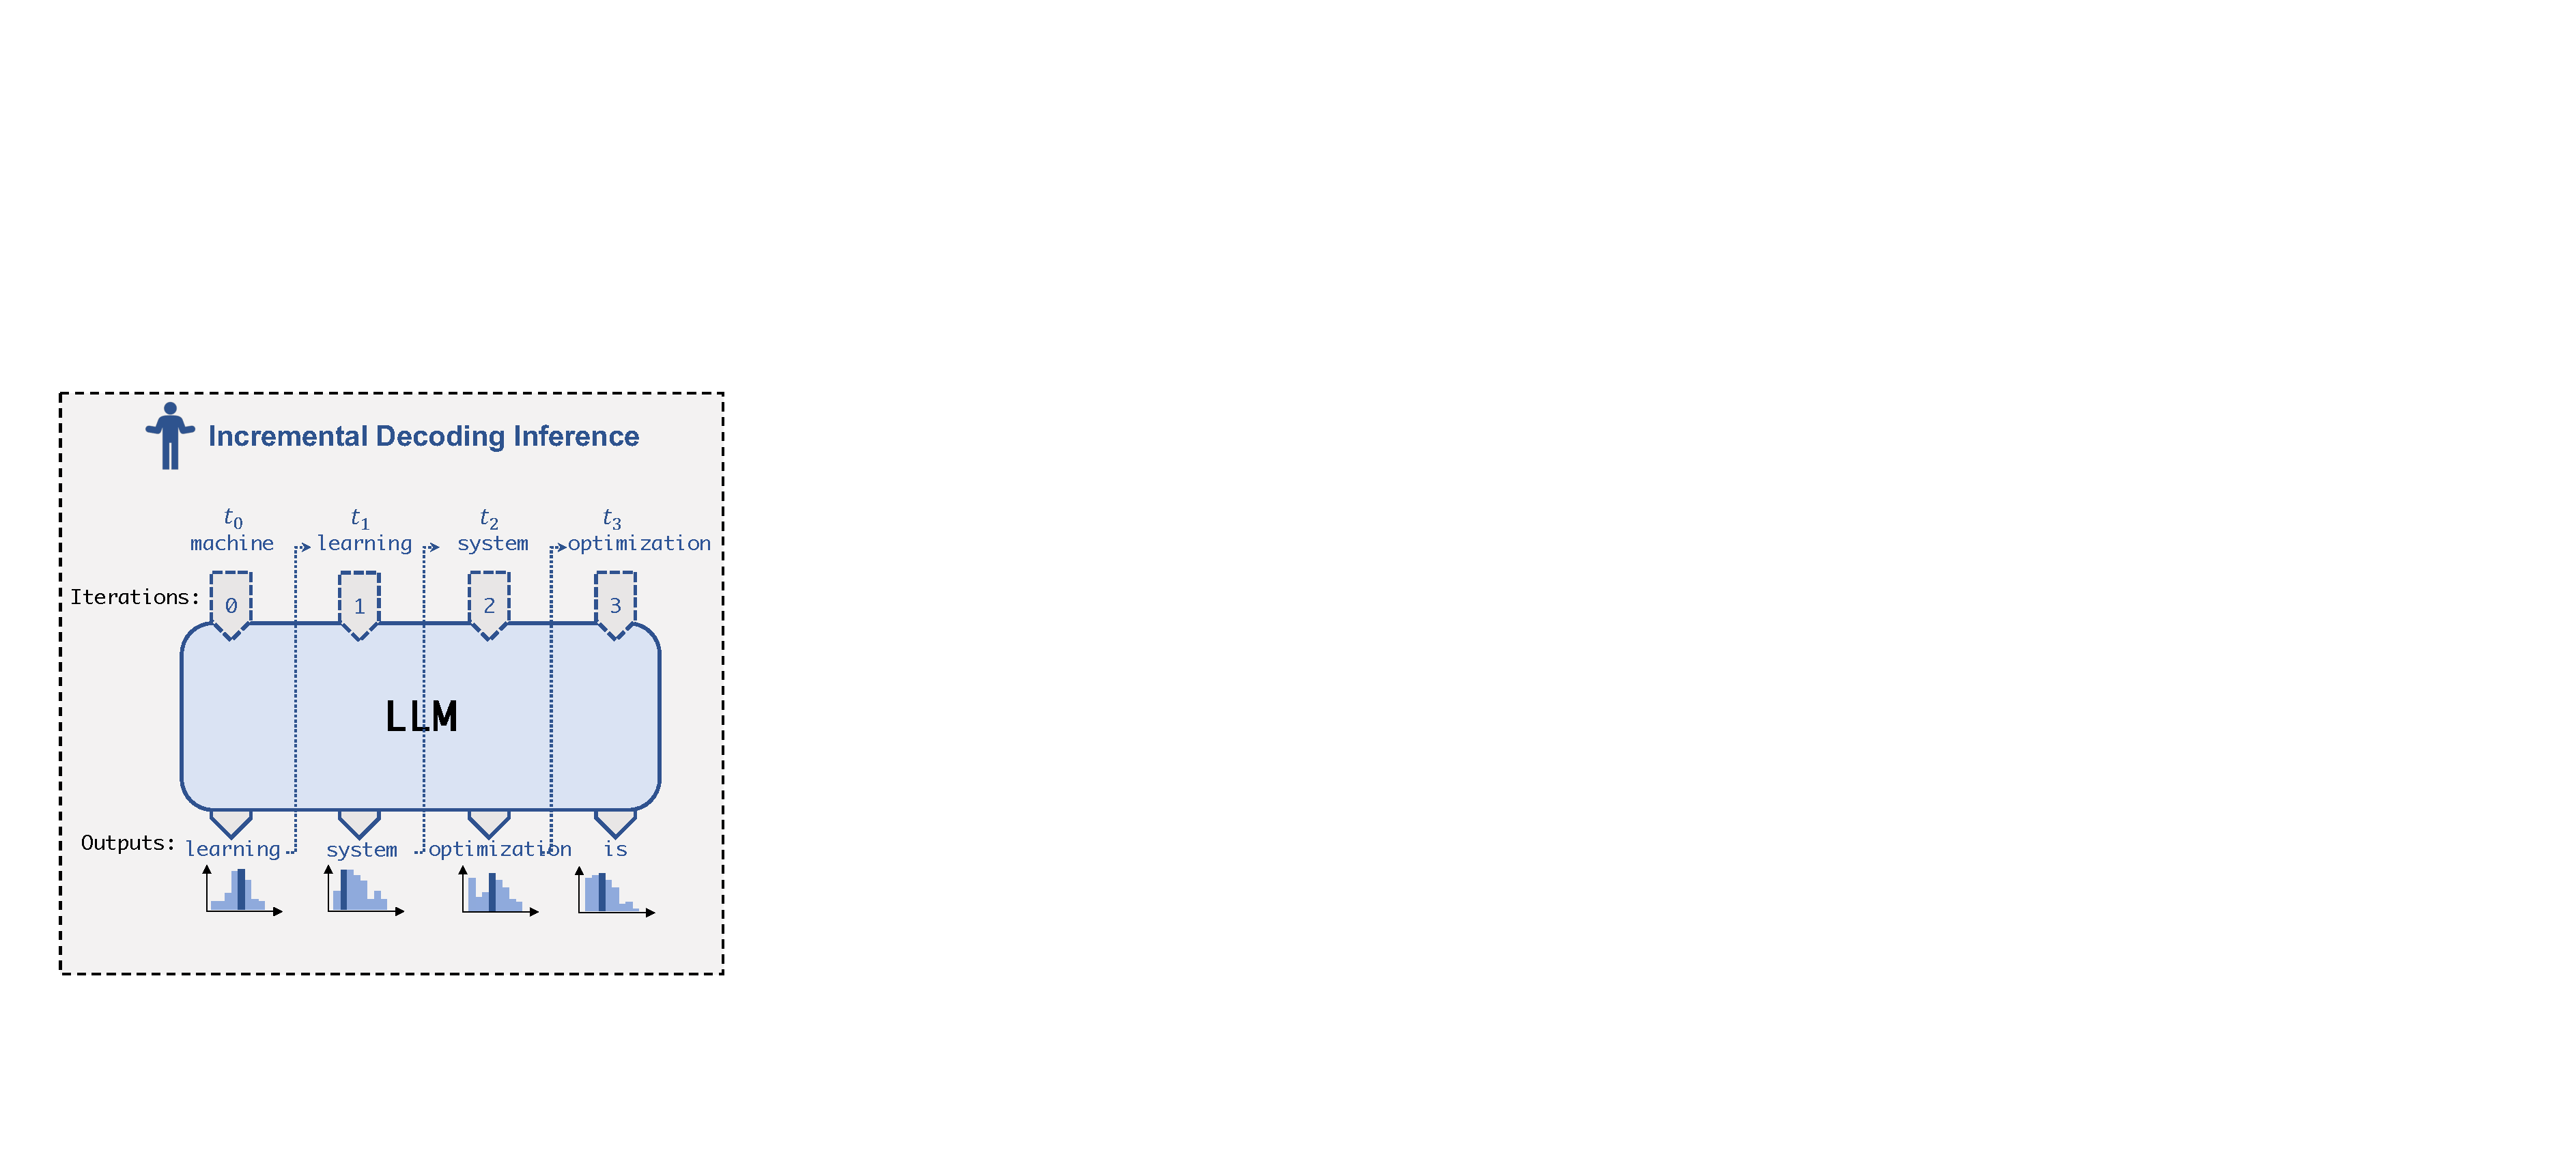
\includegraphics[scale=0.42]{rebuttal_figs/existing_overview6a3.pdf}
%     \label{fig:existing_approach}
%     }
%     \subfloat[\rev{Timeline Comparison.}]{
%     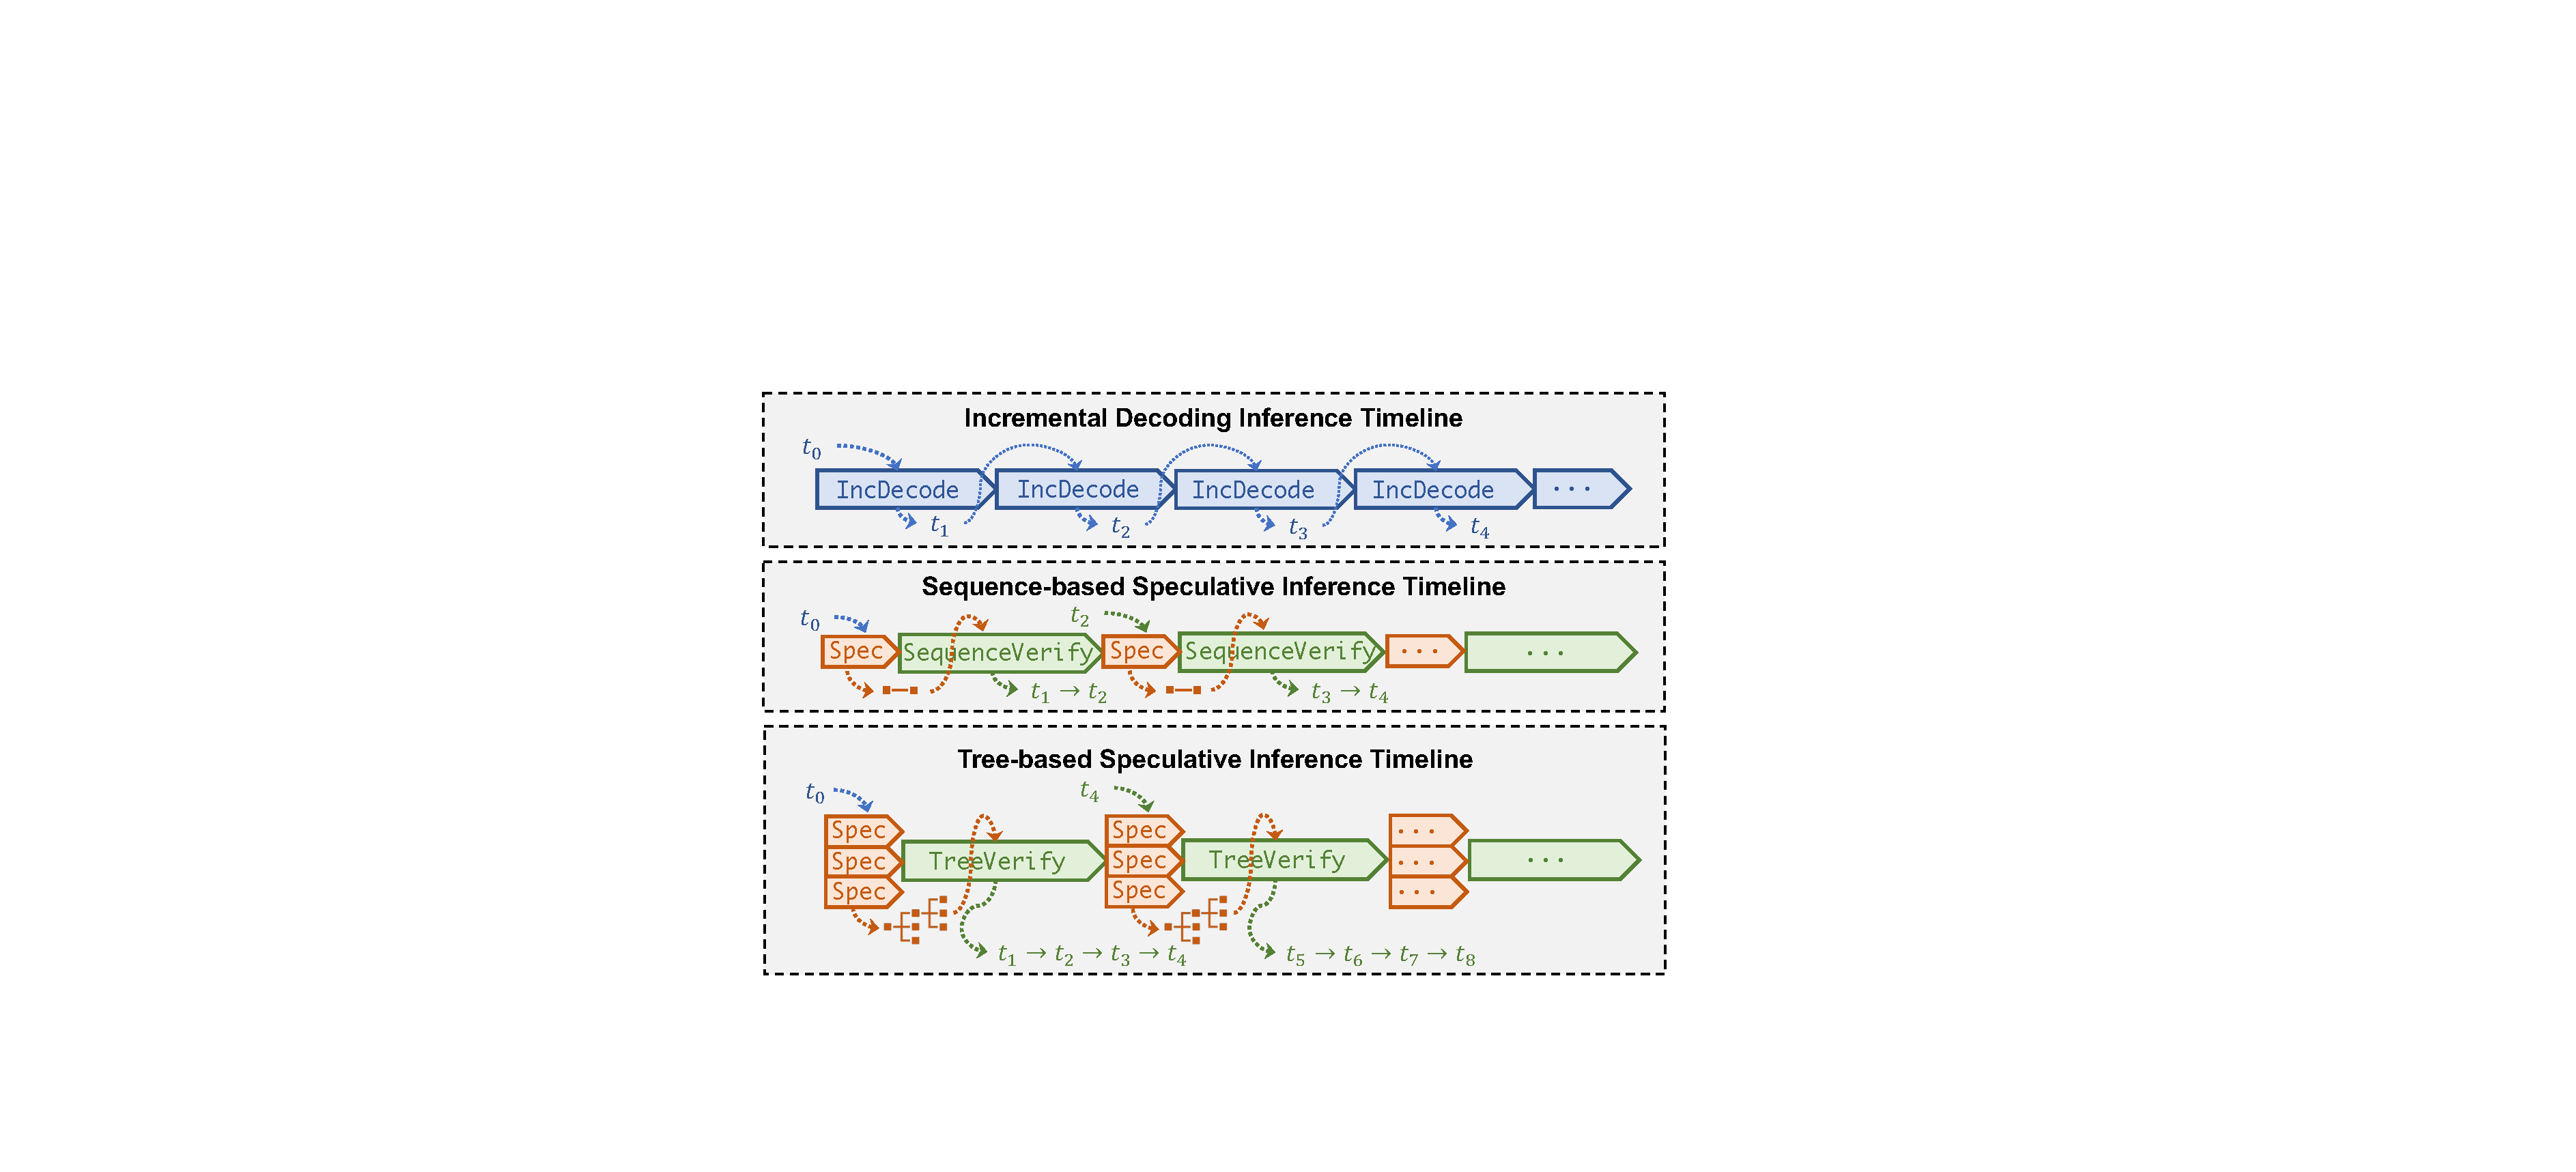
\includegraphics[scale=0.42]{rebuttal_figs/existing_overview6b5.pdf}
%     \label{fig:timeline}
%     }\\
%     \subfloat[\rev{Tree-based speculative inference and verification.}]{
%     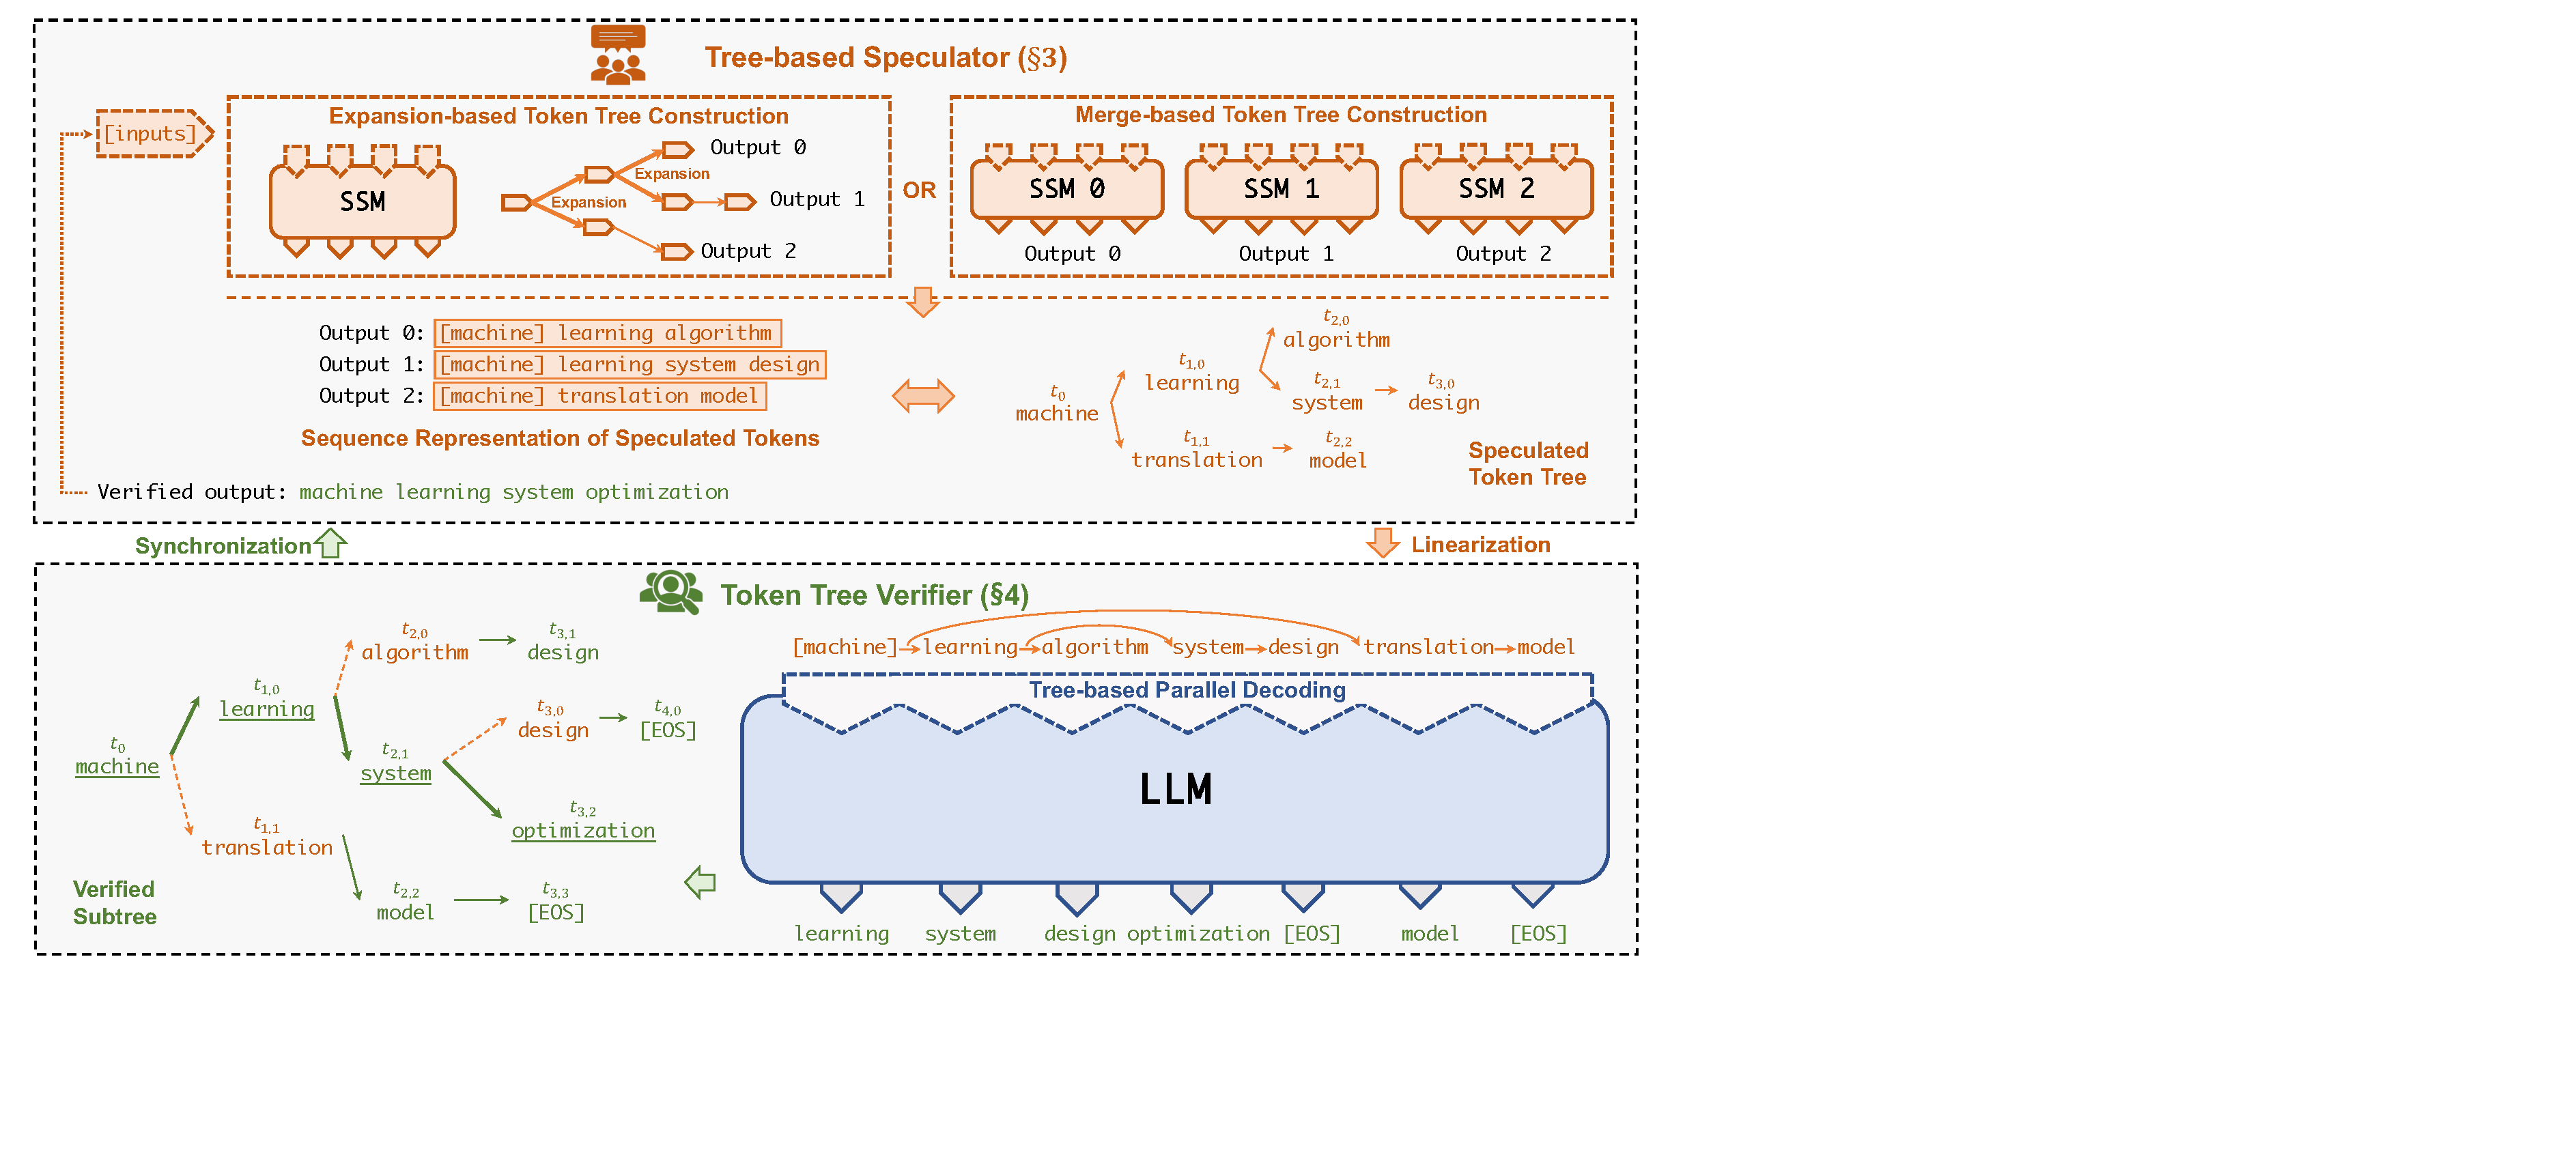
\includegraphics[scale=0.42]{rebuttal_figs/speculative_inference_overview8.pdf}
%     \label{fig:speculative_inference}
%     }
%     \caption{Comparing the incremental decoding approach used by existing LLM serving systems and the speculative inference and token tree verification approach used by \sys. \XM{Thinking to move figure (c) to page 3 or 4 as a separate overview figure}. \ZJ{I think that's a good idea. Can we also highlight the difference between existing sequence-based speculation and our proposed tree-based speculation?}}
%     \label{fig:specinfer_compared_to_incr_decoding}
% \end{figure*}

\begin{figure*}
    \centering
    \subfloat[Incremental decoding.]{
    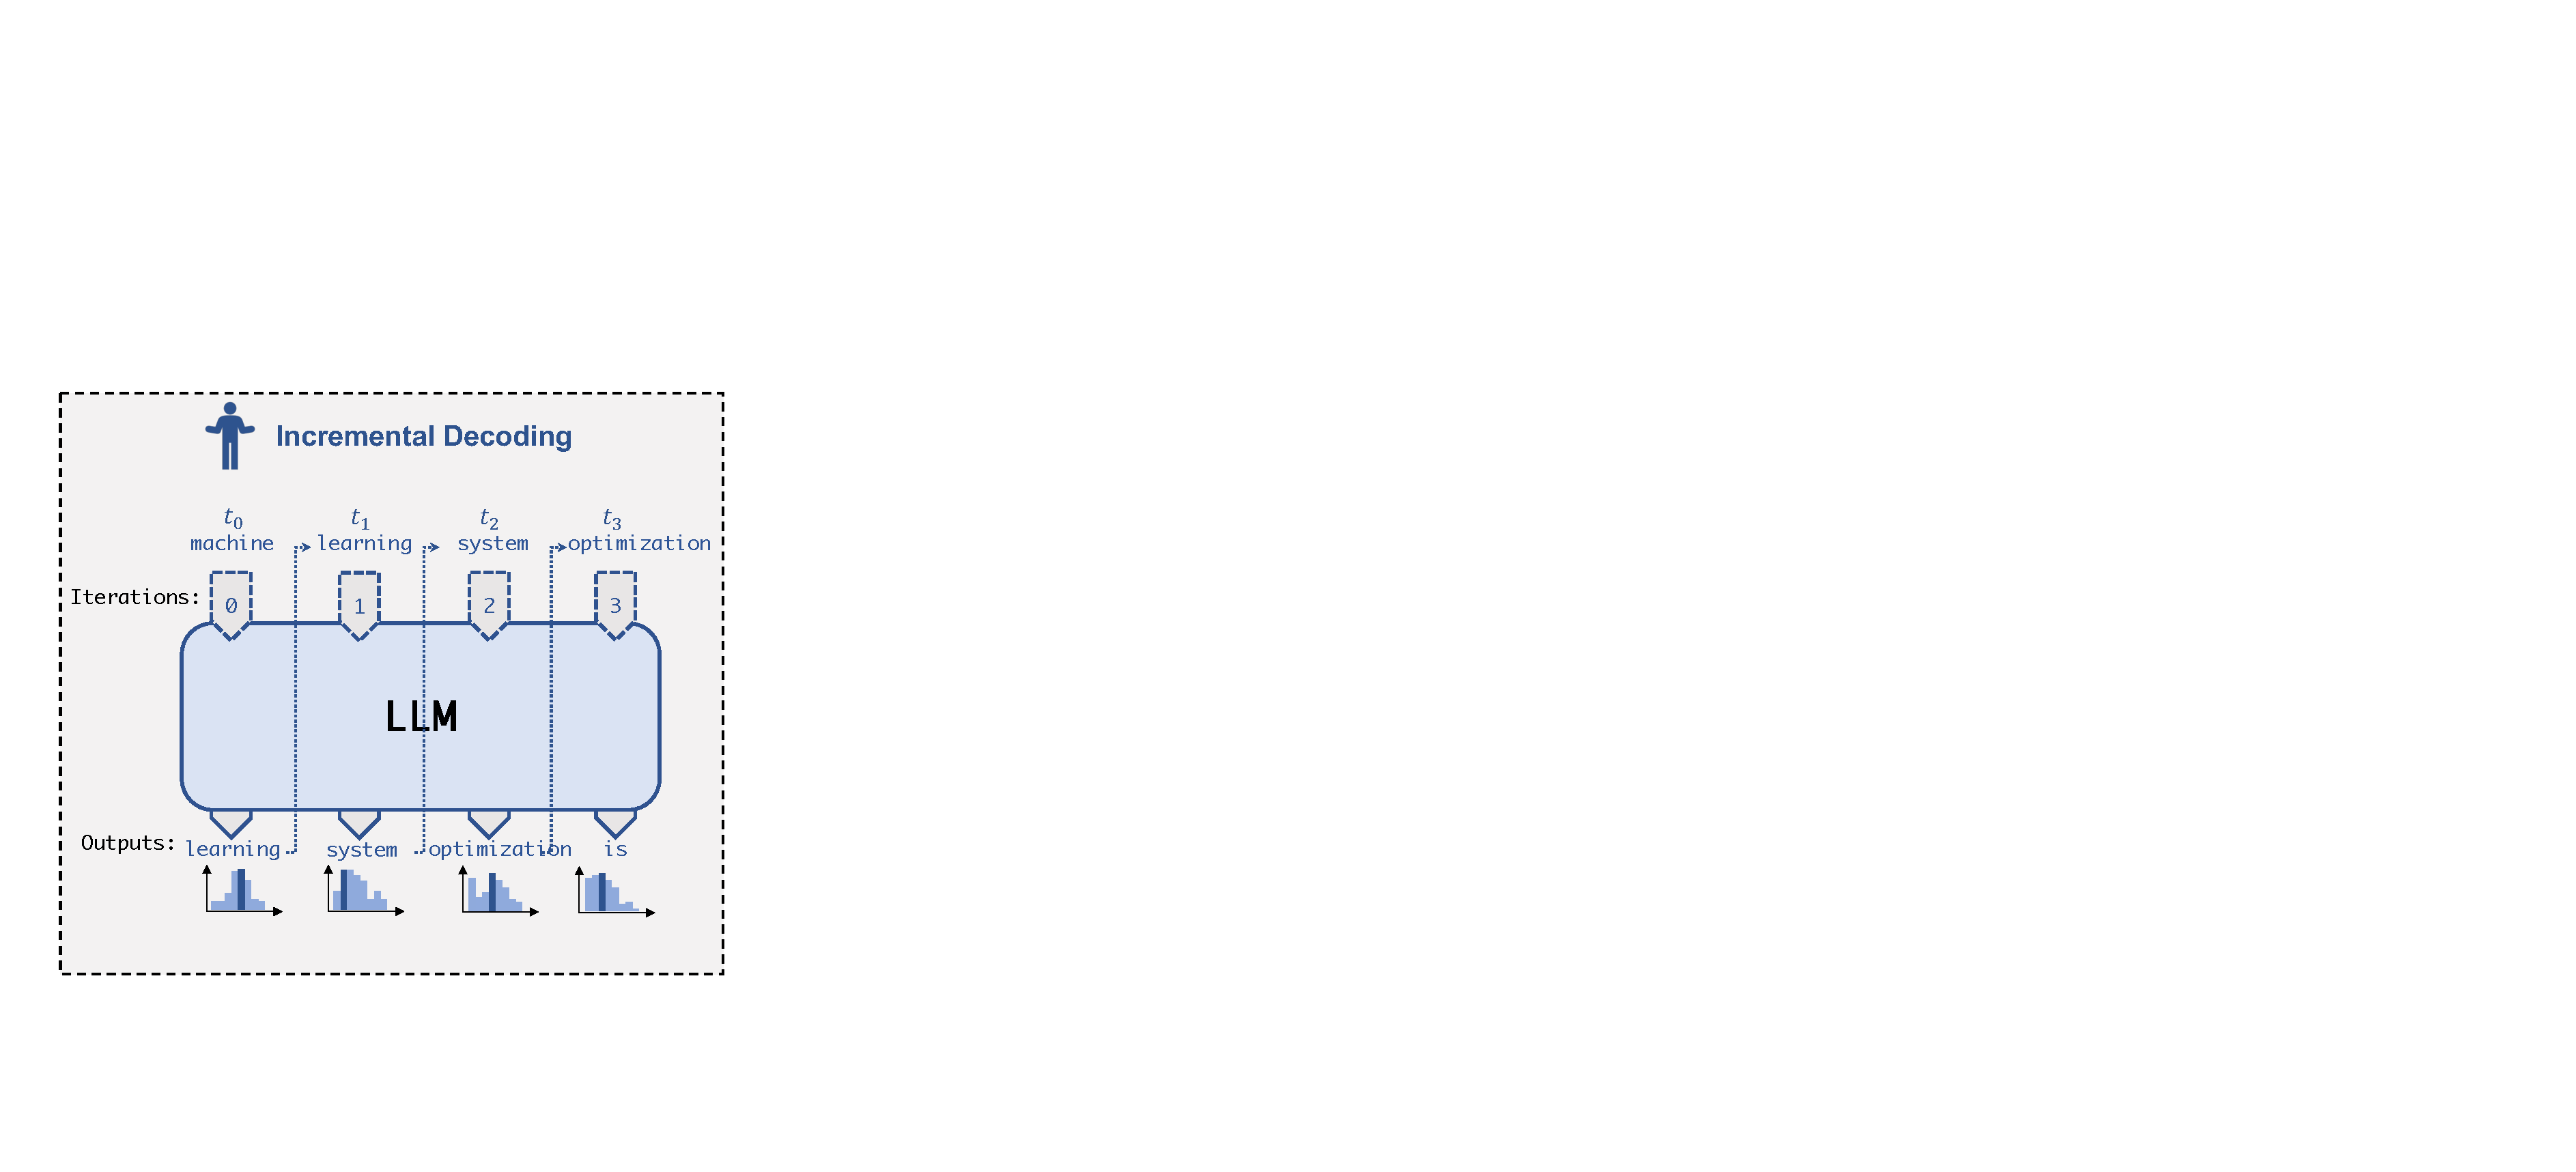
\includegraphics[scale=0.40]{rebuttal_figs/existing_overview6a4.pdf}
    \label{fig:existing_approach}
    }
    \subfloat[\rev{Timeline Comparison.}]{
    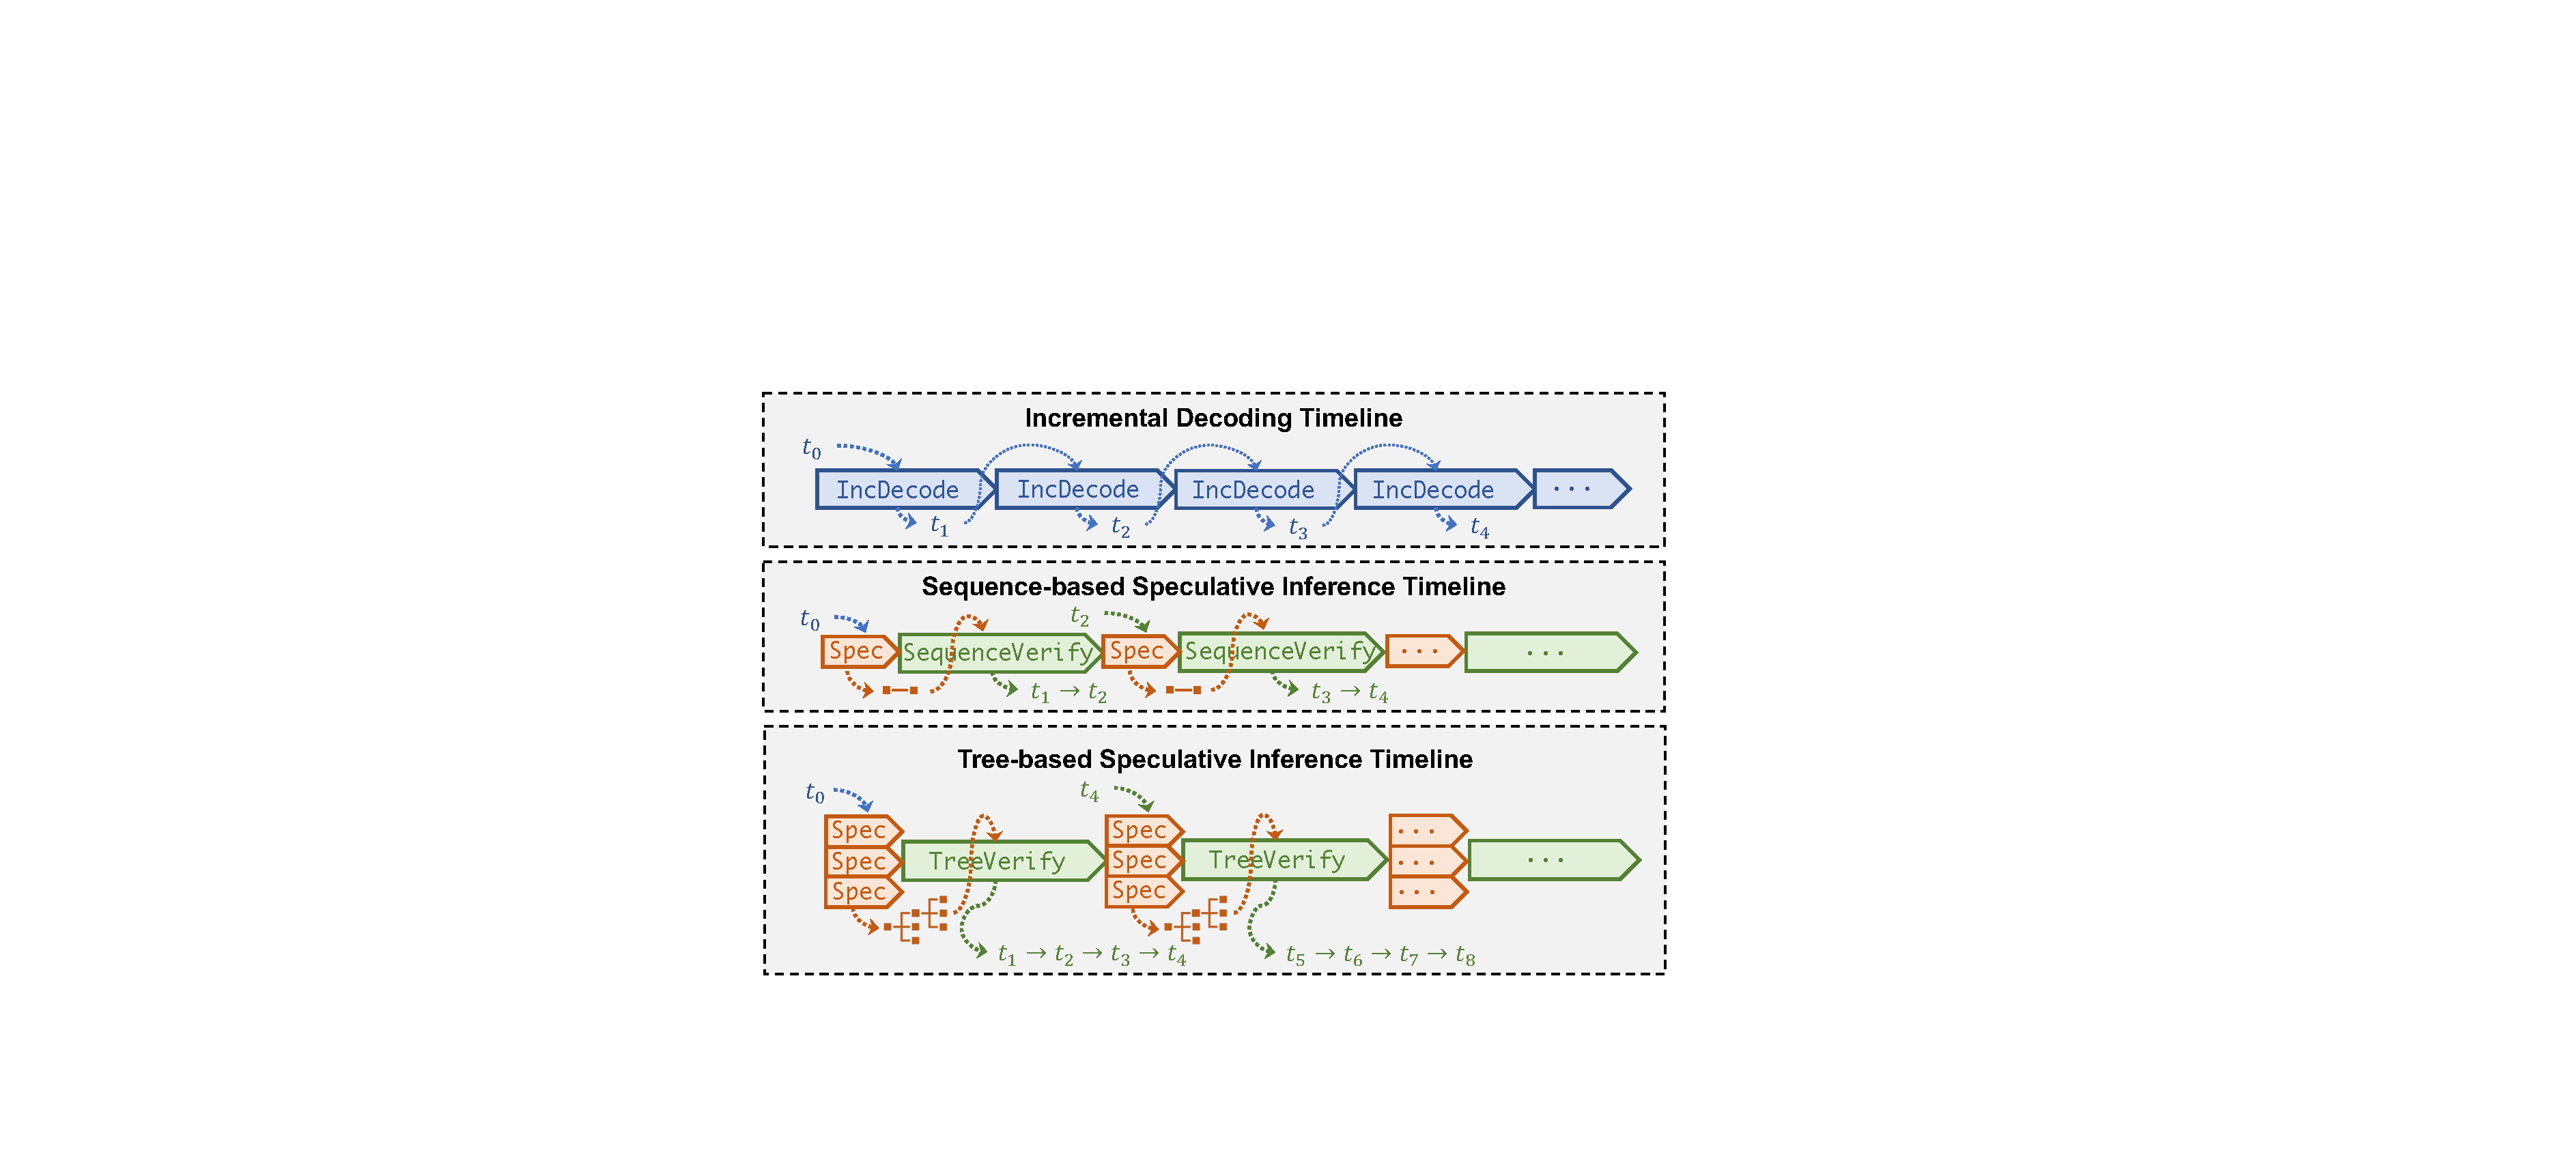
\includegraphics[scale=0.40]{rebuttal_figs/existing_overview6b6.pdf}
    \label{fig:timeline}
    }
    % \vspace{-4mm}
    \caption{\rev{Comparing the incremental decoding approach used by existing LLM serving systems, the sequence-based speculative inference approach, and the tree-based speculative inference approach used by \sys.}}
    \label{fig:specinfer_compared_to_incr_decoding}
\end{figure*}

Existing LLM systems generally use an {\em incremental decoding} approach to serving a request where the system computes the activations for all prompt tokens in a single step and then iteratively decodes {\em one} new token using the input prompt and all previously generated tokens~\cite{miao2023towards}. 
%%%
This approach respects data dependencies between tokens, but achieves suboptimal runtime performance and limited GPU utilization, since the degree of parallelism within each request is greatly limited in the incremental phase.
%%%
In addition, the attention mechanism of Transformer~\cite{vaswani2017attention} requires accessing the keys and values of all previous tokens to compute the attention output of a new token.
To avoid recomputing the keys and values for all preceding tokens, today's LLM systems use a caching mechanism to store their keys and values for reuse in future iterations.
For long-sequence generative tasks (e.g., GPT-4 supports up to 32K tokens in a request), caching keys and values introduces significant memory overhead, which prevents existing systems from serving a large number of requests in parallel due to the memory requirement of caching their keys and values.

\rev{Motivated by the idea of speculative execution in processor optimizations~\cite{gabbay1996speculative, smith1998study}, recent work introduces {\em sequence-based speculative inference}, which leverages a {\em small speculative model} (SSM) to generate a sequence of tokens and uses an LLM to examine their correctness in parallel~\cite{leviathan2022fast, xiaspeculative, stern2018blockwise, chen2023accelerating, gante2023assisted}.
%
These attempts only consider a token sequence generated by a single SSM for speculation, which cannot align well with an LLM due to the model capacity gap between them, since SSMs are generally orders of magnitude smaller than the LLM to maintain low memory and runtime overheads.
%Using a larger model can achieve better speculative performance but also introduces higher memory and runtime overheads.
}
%

%that iteratively decodes a {\em single} token using all previous tokens, as shown in \Cref{fig:existing_approach}. This approach achieves suboptimal performance and limited GPU utilization for serving LLMs since 

%This autoregressive inference approach achieves suboptimal performance and limited GPU utilization for two reasons. 
%%%
%First, unlike LLM training tasks where an ML system can simultaneously process {\em all} tokens of each training sample, a generative LLM serving system can only process {\em one} token at a time, which significantly limits the degree of parallelism within each request.
%Second, the attention mechanism of Transformer requires accessing the keys and values of all prompt tokens and previously generated tokens to compute a representation for the new token. To avoid recomputing the keys and values of all preceding tokens, {\em incremental decoding}~\cite{fiarseq} has been commonly used in modern LLM inference system to cache the keys and values for reuse in future iterations. 
%For long-sequence generative tasks, caching the keys and values introduces significant memory overhead, which prevents existing LLM inference system from serving a large number of requests in parallel due to caching keys and values.

This paper introduces \sys, a system that improves the end-to-end latency and computational efficiency of LLM serving with {\em tree-based speculative inference and verification}.
\Cref{fig:timeline} illustrates a comparison between existing incremental decoding, sequence-based speculative inference, and our tree-based speculative inference.
A key insight behind \sys is to simultaneously consider a diversity of speculation candidates (instead of just one as in existing approaches) to maximize speculative performance.
%construct a tree of speculated candidates by exploiting diversity with a single SSM and across multiple SSMs.
%combine multiple SSMs to collectively predict the LLM's outputs. \XM{TODO: update}
%
These candidates are organized as a {\em token tree}, whose nodes each represents a sequence of speculated tokens.
%
The correctness of {\em all} candidate token sequences is verified against the LLM in parallel, which allows \sys to significantly increase the number of generated tokens in an LLM decoding step. 
%combine various collectively boost-tuned small speculative models (SSMs) to jointly predict the LLM's output and use the LLM to verify {\em all} predictions, which allows \sys to opportunistically decode multiple tokens in an LLM decoding step, while existing incremental decoding approach only generates one token in each step.
%%%
%The idea of {\em speculative execution} has been widely deployed in a variety of optimization tasks in computer architecture and systems, including branch prediction in modern pipelined processors and value prediction for pre-fetching memory and files~\cite{gabbay1996speculative, smith1998study}.
\rev{Compared with sequence-based speculative inference, leveraging tree structures can significantly improve the success rate of verifying a token (e.g., from 52-57\% to 96-97\% for stochastic decoding as shown in \Cref{tab:acceptance-rate}).}
%
However, realizing this improvement requires addressing two unique challenges. Next, we elaborate on these challenges and the main ideas \sys uses to address them.

First, \sys must explore an extremely large search space of candidate token sequences to maximize speculative performance. While the idea of speculative execution has been widely deployed in a variety of optimization tasks in computer architecture and systems, including branch prediction in modern pipelined processors and value prediction for pre-fetching memory and files~\cite{gabbay1996speculative, smith1998study}, the search space considered by \sys is significantly larger due to two reasons:
%However, speculative inference requires exploring a significantly larger search space than prior speculative techniques due to two reasons:
(1) modern LLMs generally involve very large vocabularies, and (2) maximizing speculative performance requires predicting multiple future tokens (instead of just the next token). For example, all LLMs in the OPT model family consider 50,272 different possible tokens in their vocabulary, while \sys can correctly predict the next 4 tokens on average. Achieving this goal requires considering a search space of $50272^4\approx6\times 10^{18}$ different combinations of tokens. 
%Even with a set of effectively pruned speculations within the large search space, the second challenge is to verify the correctness of the speculations against the LLM efficiently.

\sys leverages existing distilled, quantized, and/or pruned variants of an LLM, which we call small speculative models (SSMs), to guide speculation. 
%
A key challenging of using SSMs for speculative inference is that the alignment between an SSM and an LLM is inherently bounded by the model capacity gap, since an SSM is generally 100-1000$\times$ smaller than an LLM.
%
\rev{Instead of using a single SSM for sequence-based speculation, \sys maximizes speculative performance by simultaneously considering a variety of token sequences organized in a tree structure for a given input prompt.
%
\Sys introduces an {\em expansion}- and a {\em merge}-based mechanism for constructing token trees by exploiting diversity within a single SSM and across multiple SSMs, respectively.}
%\Sys introduces {\em collective boost-tuning} to cooperatively fine-tune a set of SSMs by aligning their {\em aggregated} prediction with the LLM, and combines these boost-tuned SSMs to jointly predict the LLM's output. \XM{TODO: update}
%


A second challenge \Sys must address is verifying the speculated tokens. Many LLM applications perform {\em stochastic decoding}, which samples the next token from a probability distribution instead of deterministically generating a token. 
%%%
To preserve an LLM's generative performance, \Sys must guarantee that its tree-based speculative inference and verification mechanism generates the next token by following the {\em exact same} probability distribution as incremental decoding.
%%%
To achieve this goal, we propose {\em multi-step speculative sampling}, a new sampling approach for SSMs that guarantees equivalence while maximizing the number of speculated tokens that can be verified.
%%%
To minimize the token tree verification cost, \sys introduces a {\em tree-based parallel decoding} mechanism, {\em simultaneously} verifying all tokens of a token tree against the LLM's output in a {\em single} LLM decoding step.

\if 0
To this end, we introduce two key techniques to maximize \sys's speculative performance. 
%%%
For a given prefix as the input, \Sys uses multiple collectively {\em boost-tuned} small speculative models (SSMs) to jointly generate a token tree, whose nodes each represent a candidate token sequence.
%\XM{a candidate token or a candidate token sequence?}\ZJ{A token sequence. Does a candidate sequence of tokens work better here?}.
%%%
The correctness of {\em all} token sequences represented by a token tree is then verified against the LLM's original output in parallel using a novel {\em tree-based parallel} decoding algorithm.
This approach allows \Sys to opportunistically verify multiple tokens in a single decoding step as long as the speculated token tree overlaps with the LLM's output.
\fi 
%\Sys then uses an LLM as a {\em token tree verifier} that verifies whether a speculated token tree overlaps with the token sequence generated by the LLM using incremental decoding.
%%%
%\Sys is able to verify {\em all} sequences represented by a token tree in parallel and can opportunistically decode multiple tokens in a single step.

By leveraging tree-based speculative inference and verification, \Sys accelerates both distributed LLM inference across multiple GPUs and offloading-based LLM inference on one GPU.
Our evaluation shows that \Sys outperforms existing LLM serving systems by 1.5-2.8$\times$ for distributed LLM inference and by 2.6-3.5$\times$ for offloading-based LLM inference, while preserving the same generative accuracy.
%
%\rev{We will make \sys publicly available after the ASPLOS review period to facilitate future research.}

To summarize, we make the following contributions:
\begin{itemize}
    \item We present \sys, a tree-based speculative inference and verification system for LLM serving.
    \item To maximize speculative performance, we propose a merge- and an expansion-based method to construct token trees by exploiting diversity within and across SSMs, respectively.
    \item To minimize verification cost, we introduce a tree-based parallel decoding mechanism to simultaneously verify all tokens of a token tree.
    \item We evaluate \sys and show that it outperforms existing systems by up to 2.8$\times$ for distributed inference and by up to 3.5$\times$ for offloading-based inference.
\end{itemize}


\if 0
%%%
Compared to incremental decoding, \Sys's speculative inference and token tree verification introduce small computation and memory overheads for generating and verifying speculated token trees.
%%%
However, by maximizing the number of tokens that can be successfully verified in a single LLM decoding step, \Sys greatly reduces the end-to-end inference latency and improves the computational efficiency for serving generative LLMs.
%reduce memory accesses to the LLM's parameters whenever the overlap between the speculated token tree and the LLM's output is not empty.
%%%
%Since the performance of LLM inference on modern GPUs is largely limited by accessing GPU device memory, \Sys's approach can also reduce LLMs' end-to-end inference latency.
%%%
We evaluate \Sys on two LLM families (i.e., \llama~\cite{touvron2023llama} and OPT~\cite{zhang2022opt}) and five prompt datasets. 
%%%
Our evaluation shows that \Sys can reduce the number of LLM decoding steps by up to $4.4\times$ ($3.7\times$ on average) and reduce the end-to-end inference latency by up to 2.8$\times$.
\fi 

\if 0
\begin{figure}
    \centering
    \subfloat[Incremental decoding]{
    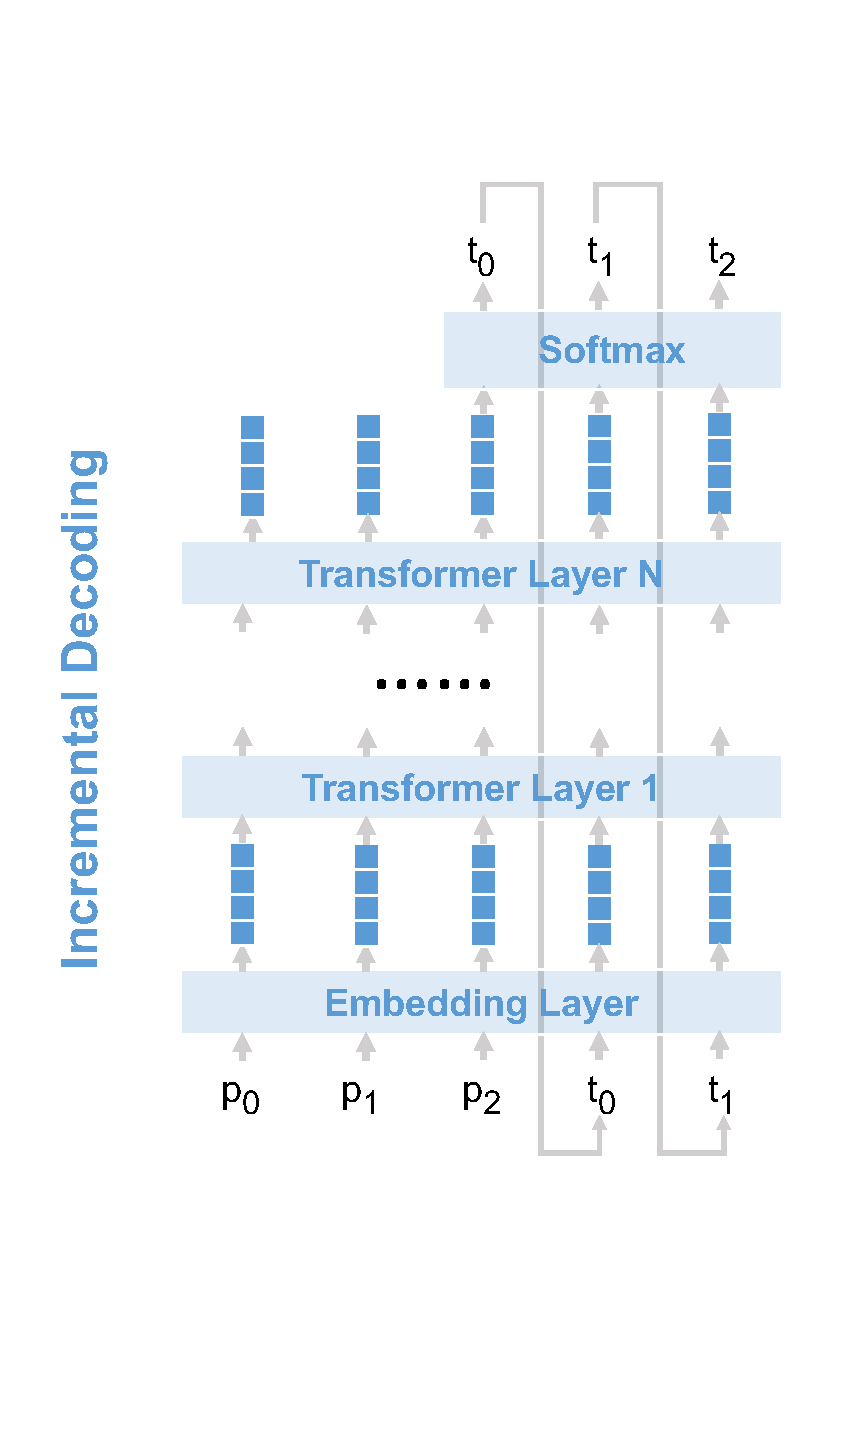
\includegraphics[scale=0.36]{figs/existing_overview.pdf}
    \label{fig:existing_approach}
    }
    \subfloat[Speculative inference with token tree verification.]{
    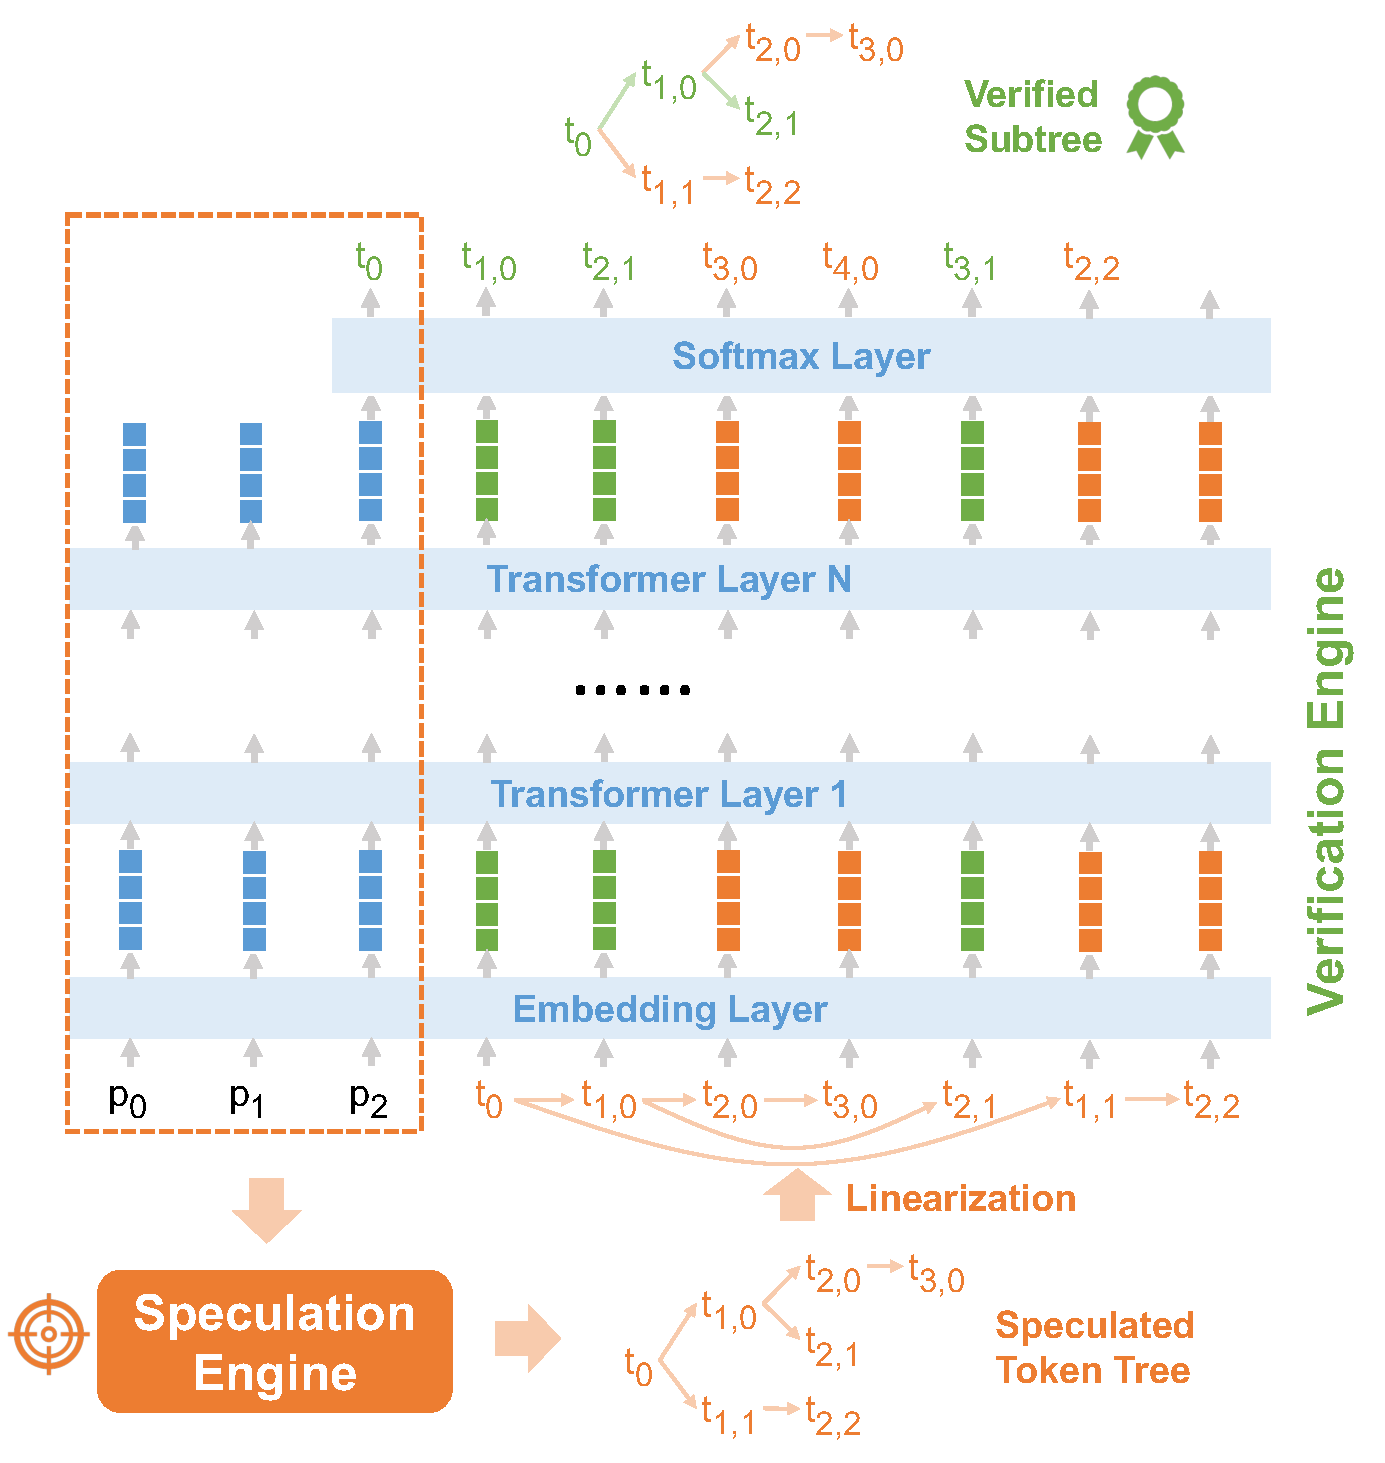
\includegraphics[scale=0.36]{figs/speculative_inference_overview.pdf}
    \label{fig:speculative_inference}
    }
    \caption{Comparing the incremental decoding approach used by existing LLM serving system and the speculative inference and token tree verification approach used by \sys.\XM{Do we want to highlight the difference between prompts and other tokens? Figure~\ref{fig:speculative_inference} might mislead the readers that the speculation engine can only accept prompts as inputs.} \ZJ{This is a great point. Any thoughts on how to improve this presentation? I am also thinking about using a real example to motivate our system.} \XM{(Done, To be replaced)}} 
\end{figure}
\fi
% \begin{figure}[t]
%     \centering
%     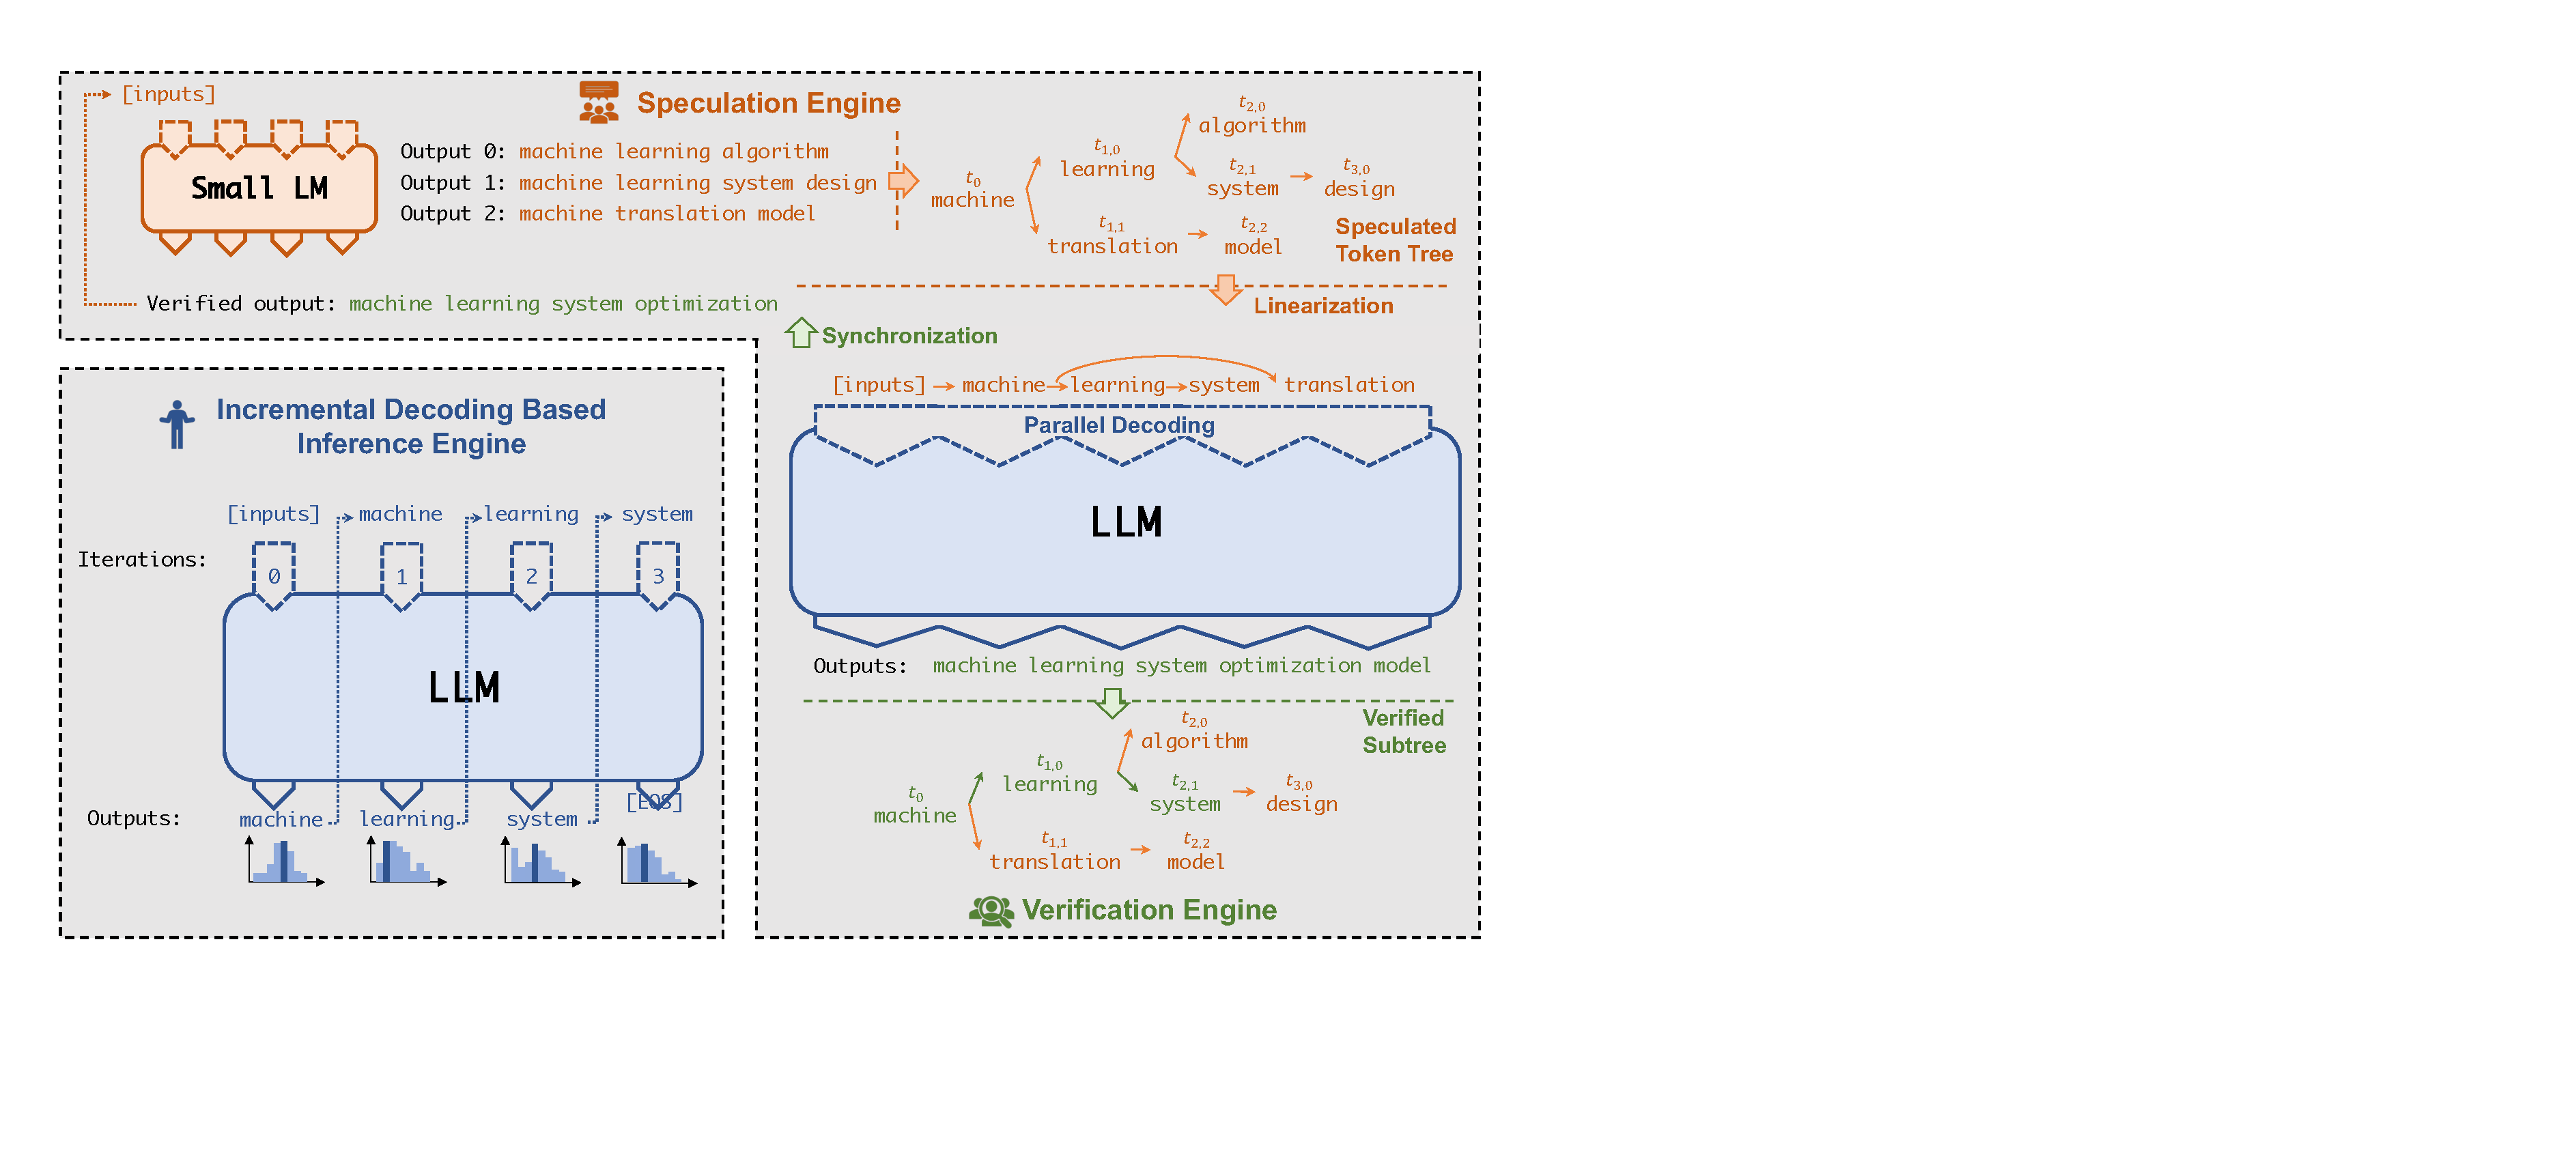
\includegraphics[width=1.0\textwidth]{figs/existing_overview4.pdf}
%     \label{fig:overview}
%     \caption{\XM{New figure}}
% \end{figure}

%\section{Background}
\label{sec:background}
\section{\Sys's Overview}
\label{sec:overview}

\begin{figure*}[t]
    \centering
    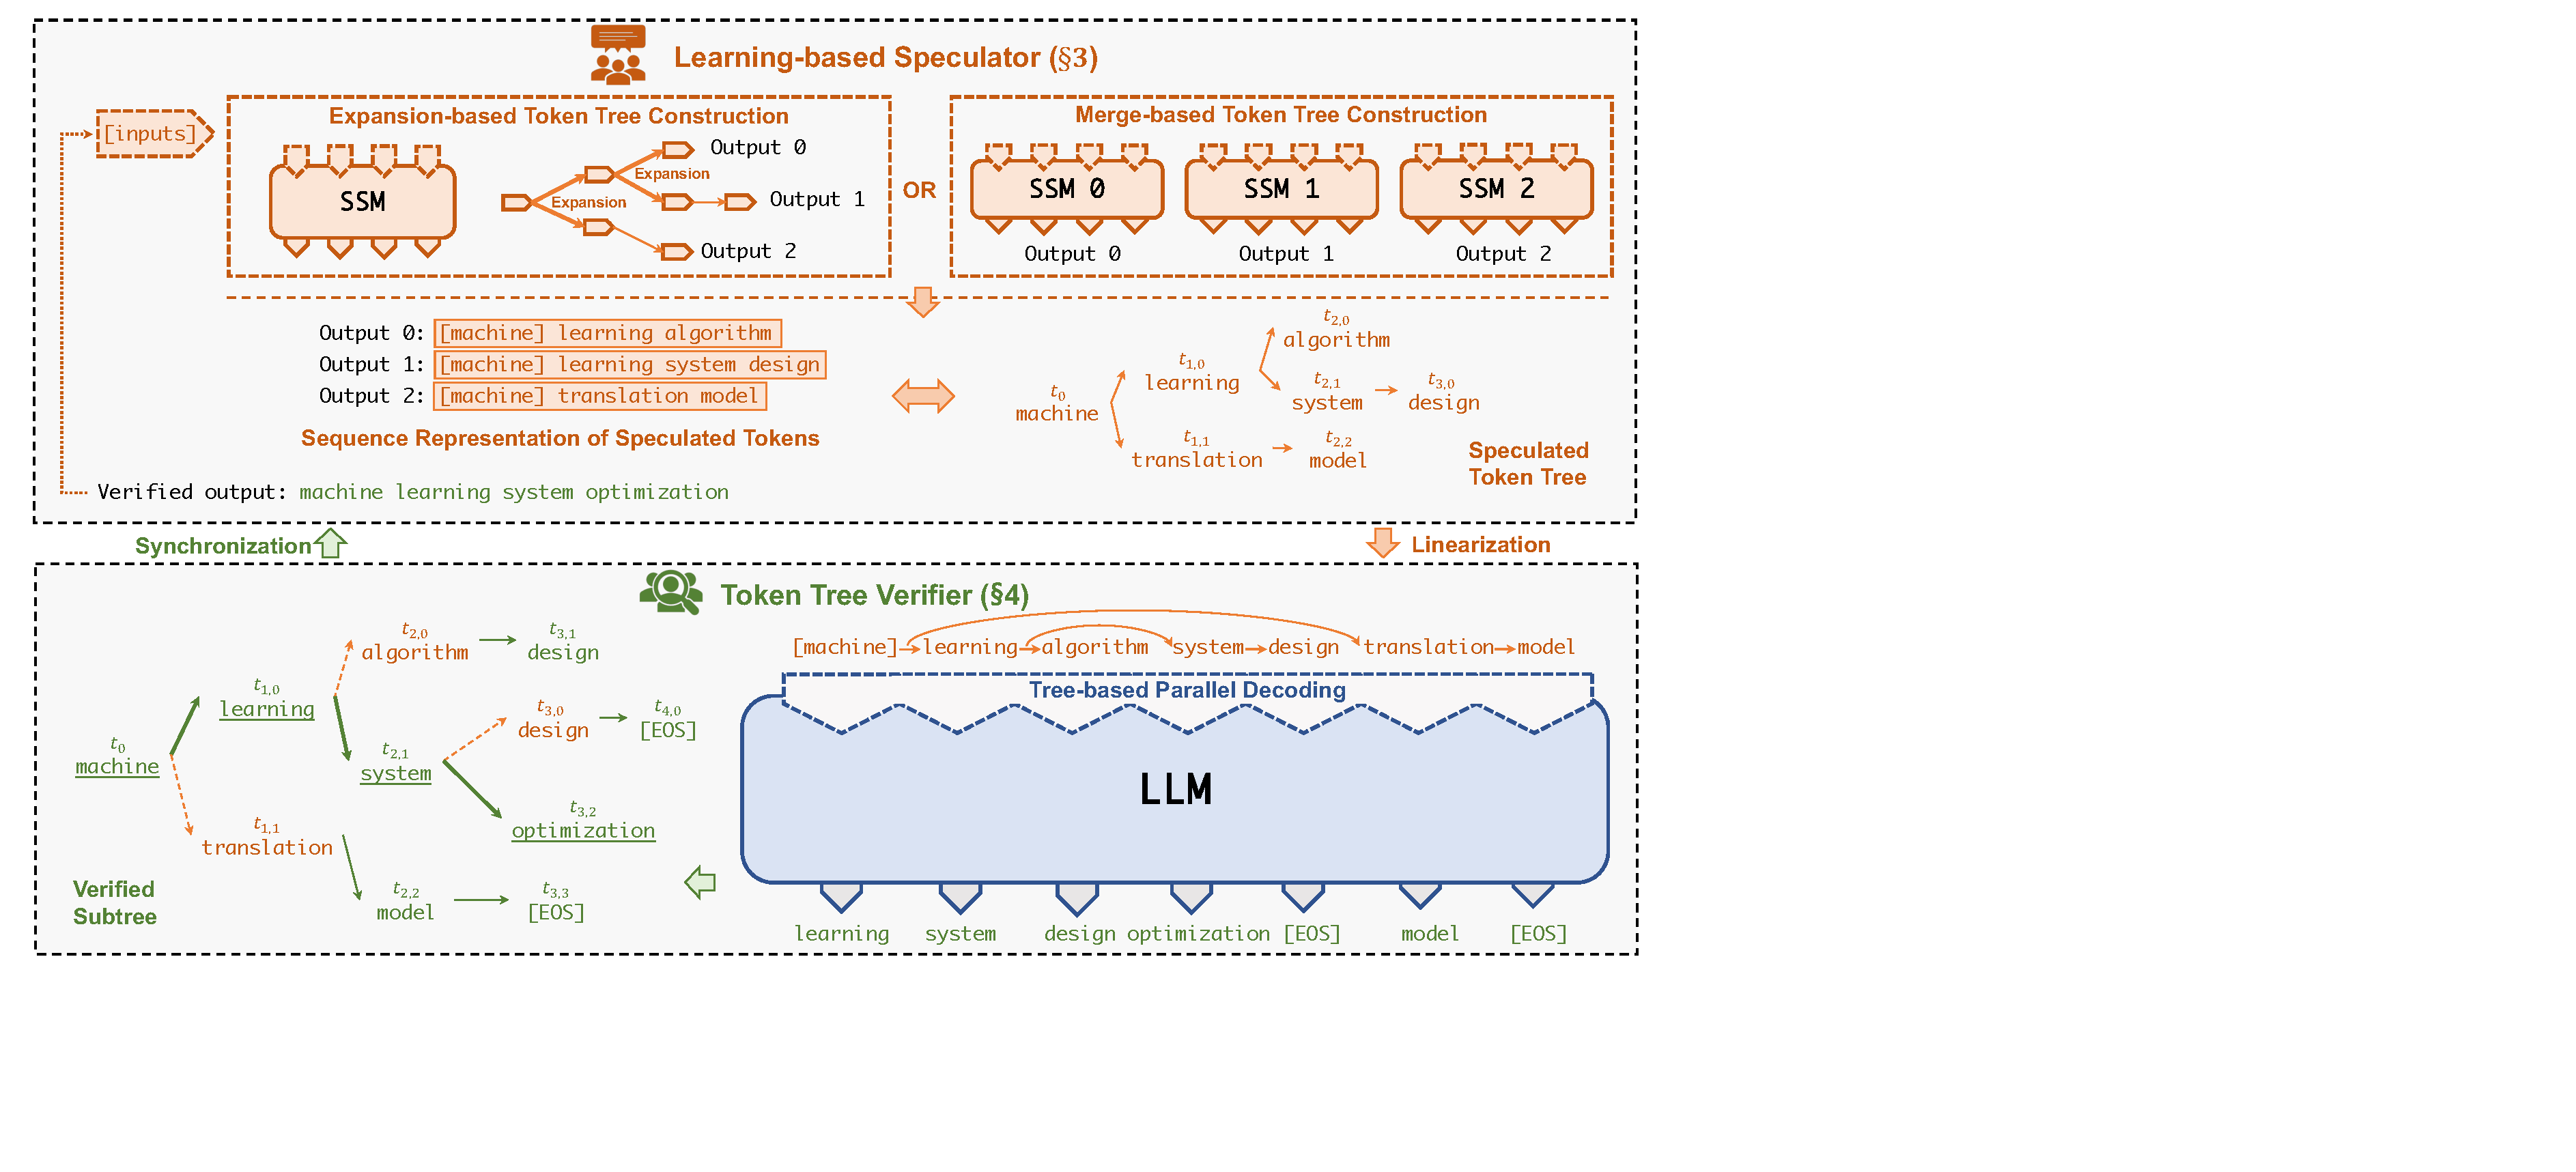
\includegraphics[scale=0.4]{rebuttal_figs/speculative_inference_overview9.pdf}
    \caption{An overview of \Sys's tree-based speculative inference and verification mechanism.}
    \label{fig:speculative_inference}
\end{figure*}


\begin{algorithm}
%\small
\caption{The incremental decoding algorithm used in existing LLM serving systems.}
\label{alg1}
\begin{algorithmic}[1]
\State {\bf Input:} A sequence of input tokens $\m{I}$
\State {\bf Output:} A sequence of generated tokens
\State $\m{S} = \m{I}$
\While{true}
\State $t = \Call{Decode}{\textrm{LLM}, \m{S}}$
\State $\m{S}$.append($t$)
\If{$t = \langle \textrm{EOS} \rangle$}
\State {\bf Return} $\m{S}$
\EndIf
\EndWhile
\end{algorithmic}
\end{algorithm}


\begin{algorithm}
%\small
\caption{The speculation and verification algorithm used by \Sys. \textproc{Speculate} takes the current token sequence $\m{S}$ as an input and generates a speculated token tree $\m{N}$. 
\textproc{TreeParallelDecode} generates a token $\m{O}(u)$ for each node $u \in \m{N}$.
%\Sys's use of an LLM is different from existing systems: the LLM takes a token tree $\m{N}$ as an input and generates a token $\m{O}(u)$ for each node $u \in \m{N}$. Note that the \textproc{TreeParallelDecode} function can generate all tokens in $\m{O}$ in a single LLM decoding step (see~\Cref{sec:verification}).
\textproc{VerifyGreedy} and \textproc{VerifyStochastic} examine $\m{N}$ against $\m{O}$ and produce a sequence of verified tokens $\m{V}$ using greedy or stochastic sampling, respectively.}
%\caption{The speculative inference and token tree verification algorithm used by \Sys.}
\label{alg2}
\begin{algorithmic}[1]
\State {\bf Input:} A sequence of input tokens $\m{I}$
\State {\bf Output:} A sequence of generated tokens
\State $\m{S} = \m{I}$
\While{true}
\State $\m{N} = \Call{Speculate}{\m{S}}$
\State $\m{O} = \Call{TreeParallelDecode}{\textrm{LLM}, \m{N}}$ 
%\XM{How about using a function that takes LLM as input to highlight the differences of using LLMs? E.g., t$\gets$Decode(LLM, S) for Algorithm 1 and $\m{O}\gets$ParallelDecode(LLM, $\m{N}$) in Algorithm 2}
\If{use greedy decoding}
\State $\m{V} = \Call{VerifyGreedy}{\m{O}, \m{N}}$
\Else
\State $\m{V} = \Call{VerifyStochastic}{\m{O}, \m{N}}$
\EndIf
\For{$t \in \m{V}$}
\State $\m{S}$.append($t$)
\If{$t = \langle \textrm{EOS} \rangle$}
\State {\bf return} $\m{S}$
\EndIf
\EndFor
\EndWhile
\State

\Function{VerifyGreedy}{$\m{O}, \m{N}$}
\State $\m{V} = \emptyset$, $u \leftarrow$ the root of token tree $\m{N}$
\While{$\exists v \in \m{N}. p_v = u \textrm{ and } t_v = \m{O}(u)$}
\State $\m{V}$.append($t_v$) 
\State $u = v$ 
\EndWhile
\State $\m{V}$.append($\m{O}(u)$)
\State {\bf return} $\m{V}$
\EndFunction
\State

\Function{VerifyStochastic}{$\m{O}, \m{N}$}
\State $\m{V} = \emptyset$, $u \leftarrow$ the root of token tree $\m{N}$
\While{$u$ is a non-leaf node}
%\State $\m{H} = \textrm{child}(u), P(x)\coloneqq P(x \mid u, \Theta_{\textrm{LLM}})$ 
\State $\m{H} = \textrm{child}(u)$
\Comment{\textcolor{violet}{The set of child nodes for $u$}}
    \While{$\m{H}$ is not empty}
    % \Comment{get $q_{i}(\cdot\mid u)$ with the smallest total variation distance w.r.t $p(\cdot\mid u)$}
    \State $s\sim \textrm{rand}(\m{H}), r \sim U(0, 1), x_s=\m{H}[s]$ 
        \If{$r \leq {P(x_s \mid u, \Theta_{LLM})} / {P(x_s \mid u, \Theta_{SSM_s})}$}
            \LineComment{\textcolor{violet}{Token $x_s$ passes verification.}}
            \State $\m{V}$.append($x_s$)
            \State $u = s$
            \State {\bf break}
        \Else            
            \LineComment{\textcolor{violet}{Normalize the residual $P(x \mid u, \Theta_{LLM})$}}
            % \LineComment{normalize the residual distribution between $q(x \mid u)$ and $p(x \mid u)$}
            \State $P(x \mid u, \Theta_{\textrm{LLM}})\coloneqq \textrm{norm}(\max(0, P(x \mid u, \Theta_{\textrm{LLM}})-P(x \mid u, \Theta_{\textrm{SSM}_s})))$ 
            \State $\m{H}.\textrm{pop}(s)$
        \EndIf   
    \EndWhile
\If{$\m{H}$ is empty}
    \State {\bf break}
\EndIf
\EndWhile
\LineComment{All SSMs fail verification; sample the next token}
\State $x_{\textrm{next}} \sim P(x \mid u, \Theta_{LLM})$
\State $\m{V}$.append($x_{\textrm{next}}$)
\State {\bf return} $\m{V}$

\EndFunction
\end{algorithmic}
\end{algorithm}

% \Cref{fig:specinfer_compared_to_incr_decoding} shows an overview of \sys in comparison with incremental decoding.
\Cref{fig:speculative_inference} shows an overview of \sys, which
includes a {\em learning-based speculator} that takes as input a sequence of tokens, and produces a {\em speculated token tree}.
%%%
The goal of the speculator is to predict the LLM's output by maximizing the overlap between the speculated token tree and the tokens generated by the LLM using incremental decoding (Alg.~\ref{alg1}).
%tokens that will be generated by the LLM and maximizes the likelihood that the speculated token tree includes the true token sequence.
%%%
% As shown at the top of \Cref{fig:speculative_inference}, the speculator combines multiple distilled and/or pruned versions of the LLM, which we call small speculative models (SSMs).\XM{TODO: update}
%%%

There are several ways to prepare SSMs for speculative inference. 
First, modern LLMs generally have many smaller architectures pre-trained together with the LLM using the same datasets. 
%%%
For example, in addition to the OPT-175B model with 175 billion parameters, the OPT model family also includes OPT-125M and OPT-350M, two variants with 125 million and 350 million parameters, which were pre-trained using the same datasets as OPT-175B~\cite{zhang2022opt}.
%%%
These pre-trained small models can be directly used as SSMs. 
\rev{Second, to improve the coverage of speculated tokens from SSMs, \Sys takes an expansion-based and a merge-based speculation method as shown at the top of \Cref{fig:speculative_inference}. The speculated tokens are organized in a token tree structure.}
% \rev{\Sys takes an expansion-based mechanism for constructing a token tree from a single SSM.}
% Second, to further improve the coverage of speculated token trees, \Sys also introduces a fine-tuning technique called {\em collective boost-tuning} to cooperatively fine-tune a set of SSMs by aligning their aggregated prediction with the LLM's using adaptive boosting~\cite{freund1999short}.\XM{TODO: update}

\if 0
The speculator automatically combines the candidate token sequences predicted by individual SSMs to construct a token tree, as shown in \Cref{fig:speculative_inference}.
Since \sys executes multiple SSMs in parallel, using more SSMs does not directly increase the speculative inference latency.
%%%
However, using a large number of SSMs will result in a large token tree, which requires more memory and computation resources for verification.
%%%
To address this challenge, \sys uses a {\em learning-based} speculative scheduler to learn to decide which SSMs to use for a given input token sequence and the speculative configurations for these SSMs (e.g., the beam search width and depth when running an SSM using beam search).
\fi
%The speculation engine can be implemented as a combination of (1) user-provided functions that predict future tokens based on heuristics and/or retrieval-augmented documents, and (2) a collection of small, distilled versions of the LLM trained using the same dataset, and (3) fine-tuned versions of the small models on the target tasks.
%%%

\Sys's usage of an LLM is also different from that of existing LLM serving systems. 
Instead of using the LLM as an incremental decoder that predicts the next single token, \sys uses the LLM as a token tree verifier that verifies a speculated token tree against the LLM's output.
%%%
For each token, \sys computes its activations by considering all of its ancestors in the token tree as its preceding tokens.
%%%
For example, in \Cref{fig:speculative_inference}, the attention output of the token $t_{3,0}$ is calculated based on sequence $(t_0, t_{1,0}, t_{2, 1}, t_{3,0})$, where $t_0$, $t_{1,0}$, and $t_{2,1}$ are $t_{3,0}$'s ancestors in the token tree.
\Sys includes a novel tree-based parallel decoding mechanism to simultaneously verify {\em all} tokens of a token tree in a single LLM decoding step.

\Sys's speculative inference and token tree verification provide two key advantages over the incremental decoding approach of existing LLM inference systems.

\paragraph{Reduced memory accesses to LLM parameters.} The performance of  LLM inference is largely limited by accesses to GPU memory.
In the existing incremental decoding approach, generating a single token requires accessing all parameters of an LLM. 
%%%
The problem is exacerbated for offloading-based LLM inference systems, which use limited computational resources such as a single commodity GPU to serve LLMs by utilizing CPU DRAM and persistent storage to save model parameters and loading these parameters to GPU's high bandwidth memory (HBM) for computation.
Compared to the incremental decoding approach, \sys significantly reduces accesses to LLM parameters whenever the overlap between a speculated token tree and the LLM's actual output is not empty.
%Memory accesses to an LLM's parameters are significantly reduced when the speculation engine can correctly includes the actual future tokens in the speculated token tree.
%%%
Reduced accesses to GPU device memory and reduced data transfers between GPU and CPU memory can also directly translate to decreased energy consumption, since accessing GPU HBM consumes two or three orders of magnitude more energy than floating point arithmetic operations.

\paragraph{Reduced end-to-end inference latency.}
Serving LLMs suffers from long end-to-end inference latency.
For example, the GPT-3 architecture includes 175 billion parameters and requires many seconds to serve a request.
In the existing incremental decoding approach, the computation for generating each token depends on the keys and values of all previously generated tokens, which introduces sequential dependencies between tokens and requires modern LLM serving systems to serialize the generation of different tokens for each request.
%%%
In \sys, LLMs are used as a verifier that takes a speculated token tree as an input and can simultaneously examine {\em all} tokens in the token tree by making a single verification pass over the LLM. 
This approach enables parallelization across different tokens in a single request and reduces the LLM's end-to-end inference latency.

%\begin{itemize}
%    \item A figure to show that our approach applies to distributed inference case: (1) reduced end-to-end inference latency (2) reduced data transfers between GPUs
%    \item A figure to show that our approach applies to offload inference case: (1) reduced end-to-end inference latency (2) less memory accesses to load model weights from CPU DRAM
%\end{itemize}



\section{Learning-based Speculator}
\label{sec:speculation}

\if 0
\begin{figure}
    \centering
    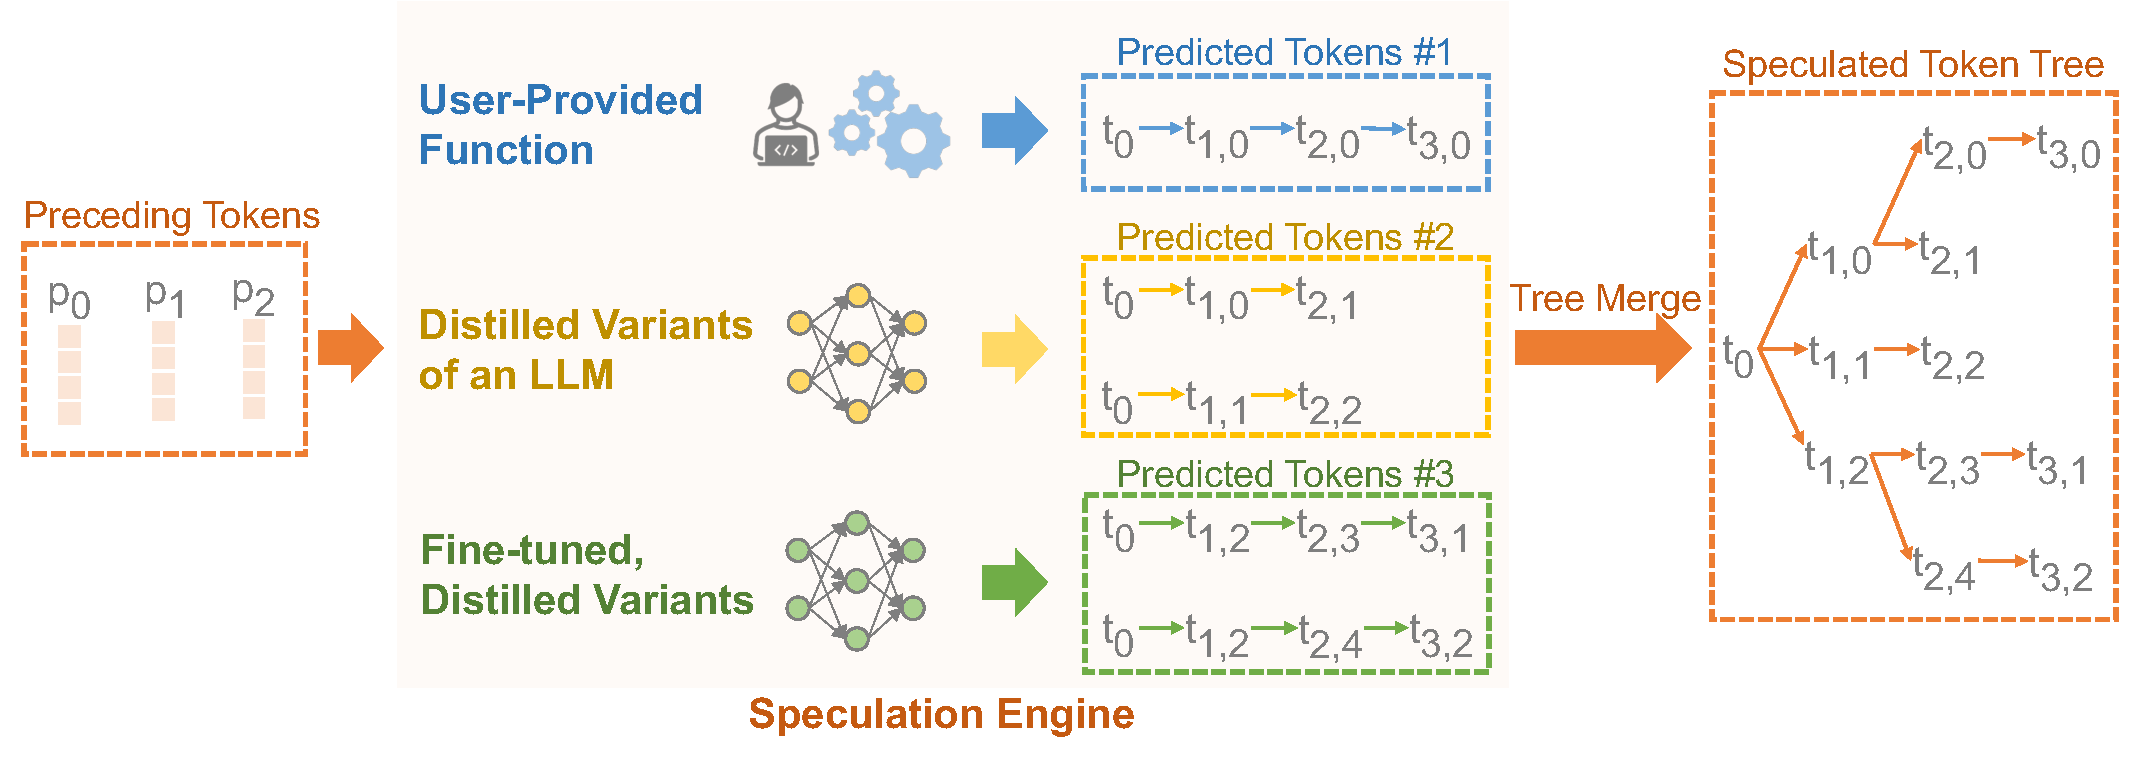
\includegraphics[scale=0.38]{figs/speculation_engine_v2.pdf}
    \caption{An overview of \Sys's speculation engine. \ZJ{To be removed}}
    \label{fig:speculation_engine}
\end{figure}
\fi

\begin{table}
\begin{center}
\caption{\rev{The success rate of verifying a token for \llama-7B using the top-$k$ tokens derived from \llama-68M. The five prompt datasets are described in \Cref{subsec:setup}.}}
%\footnotesize
\label{tab:acceptance-rate}
\begin{tabular}{l|l|ccccc}
\toprule
& Dataset     & $k=1$ & $k=2$ & $k=3$ & $k=4$ & $k=5$ \\ \midrule
\multirow{5}{*}{\rotatebox[origin=c]{90}{\parbox{2cm}{\bf \centering Greedy\\ decoding}}}
& Alpaca     &68\%          & 77\%    & 81\%     & 84\%     & 85\%     \\
& CP         &69\%          & 79\%    & 83\%     & 86\%     & 87\%     \\
& WebQA      &62\%          & 72\%    & 77\%     & 80\%     & 82\%     \\ 
& CIP        &70\%          & 81\%    & 85\%     & 88\%     & 89\%     \\
& PIQA       &63\%          & 75\%    & 79\%     & 83\%     & 85\%     \\
\midrule
\multirow{5}{*}{\rotatebox[origin=c]{90}{\parbox{2cm}{\bf \centering Stochastic\\ decoding}}}
& Alpaca     &54\%          & 81\%    & 91\%     & 95\%     & 97\%     \\
& CP         &56\%          & 82\%    & 92\%     & 95\%     & 97\%     \\
& WebQA      &52\%          & 80\%    & 90\%     & 94\%     & 96\%     \\ 
& CIP        &57\%          & 84\%    & 92\%     & 95\%     & 97\%     \\
& PIQA       &55\%          & 82\%    & 91\%     & 95\%     & 97\%     \\
\bottomrule
\end{tabular}
\end{center}
\end{table}

\if 0
Existing speculative decoding methods perform {\em sequence-based} speculation, where an SSM predicts a sequence of tokens to be verified by an LLM.
%
However, a key limitation of sequence-based speculation is that the alignment between an SSM and an LLM is inherently bounded by the model capacity gap between the two models~\cite{leviathan2022fast, stern2018blockwise}.
%%%
Our preliminary exploration shows that using a larger SSM can achieve better speculative performance at the cost of increased memory overhead and inference latency.
\fi

\rev{Existing speculative decoding methods perform {\em sequence-based} speculation, where an SSM predicts a single sequence of tokens to be verified by an LLM.
%%%
However, a key limitation of a single speculated sequence is that the probability of a successful alignment between the LLM and the speculated token sequence decays exponentially with the expected alignment length.
%%%
This can be further exacerbated by the fact that the speculation only includes a single candidate token to verify per step, resulting in suboptimal speculative performance.
%%%
On the other hand, by encouraging more diverse speculated candidates per step, the probability of a successful match per step (i.e., the token decoded by the LLM is in this candidate pool) can be greatly improved. 
%%%
To this end, \sys aims to construct a tree of speculated candidates by exploiting diversity within a single SSM and across multiple SSMs.
In particular, \sys's {\em learning-based speculator} aggregates the predictions of one or multiple SSMs to maximize speculative performance while maintaining low memory overhead and inference latency.
%
\Sys uses a {\em token tree} to organize the tokens produced by the speculator and introduces two methods for constructing token trees: {\em expansion-} and {\em merge-based} tree constructions.}
%\XM{multiple SSMs or multiple/one SSM?}

\begin{definition}[Token Tree]
A token tree $\m{N}$ is a tree structure, where each node $u \in \m{N}$ is labeled with a token $t_u$, and $p_u$ represents $u$'s parent node in the token tree. 
For each node $u$, $S_u$ represents a sequence of tokens identified by concatenating $S_{p_u}$ and $\{t_u\}$\footnote{For the root node $r$, $S_r$ represents the token sequence $\{t_r\}$.}.
\end{definition}

\rev{\paragraph{Expansion-based token tree construction.}
One approach to creating a token tree involves deriving {\em multiple} tokens from an SSM within a single decoding step.
This approach is motivated by an important observation that when an SSM misaligns with an LLM (i.e., the two models select different top-1 tokens), the token selected by the LLM is generally among the top-$k$ tokens from the SSM for very small values of $k$.
\Cref{tab:acceptance-rate} shows the success rate of verifying a token using the top-$k$ tokens derived from an SSM, where a verification is successful if the token selected by the LLM is among the top-$k$ tokens from the SSM. Compared to only using the top-$1$ token from an SSM, using the top-$5$ tokens can increase the success rate from 70\% to 89\% for greedy decoding and from 57\% to 97\% for stochastic decoding.}

%%%
\rev{Directly selecting the top-$k$ tokens at each step leads to an exponential increase in the number of potential token sequences, which substantially elevates inference latency and memory overhead. Consequently, we adopt a {\em static} strategy that expands the token tree following a preset {\em expansion configuration} represented as a vector of integers $\langle k_1, k_2, ..., k_m\rangle$, where $m$ denotes the maximum number of speculative decoding steps, and $k_i$ indicates the number of tokens to expand for each token in the $i$-th step.
%including the expansion depth and width. Here the expansion depth denotes the maximum number of speculated decoding steps and the expansion width represents the number of selected tokens in each step. 
%In this way, the amount of speculated token sequences is bounded by manageable size. 
For example, \Cref{fig:token_tree_merge} illustrates the expansion configuration $\langle 2, 2, 1 \rangle$, leading to four token sequences.
Our evaluation (see \Cref{subsec:eval_token_tree}) shows that even a simple strategy can generate highly accurate speculative results.
We acknowledge that {\em dynamically} expanding a token tree from an SSM is an opening research problem beyond the scope of this paper, which we leave as future work.}

% \textcolor{blue}{One approach to creating a token tree involves deriving multiple tokens from an SSM within a single decoding step. However, this method leads to an exponential increase in the number of potential token sequences, which substantially elevates inference latency. Consequently, we opt for a strategy where only one decoding step generates several tokens, followed by employing greedy decoding to produce the remaining tokens. 
% The specific decoding step where the SSM is induced to generate multiple tokens is termed the bifurcation point.
% The count of tokens produced during this step is called the tree width, while the position of this step in the sequence is referred to as the tree depth. As depicted in Figure X, the SSM is instructed to generate three tokens at the second decoding step. In this instance, the tree width is three, and the tree depth is two.}

\paragraph{Merge-based token tree construction.}
In addition to using a single SSM, \sys can also combine multiple SSMs to jointly predict an LLM's output. \Sys uses an unsupervised method to {\em collectively boost-tune} a pool of SSMs to align their outputs with that of the LLM by leveraging adaptive boosting~\cite{freund1999short}.
%%%
\Sys uses SSMs to predict the next few tokens that an LLM will generate, and uses general text datasets (e.g., the OpenWebText corpus~\cite{Gokaslan2019OpenWeb} in our evaluation) to adaptively align the aggregated output of multiple SSMs with the LLM in a fully unsupervised fashion.
%%%
In particular, \Sys converts a text corpus into a collection of prompt samples and use the LLM to generate a token sequence for each prompt. 
%%%
\Sys first fine-tunes one SSM at a time to the fullest and marks all prompt samples where the SSM and LLM generate identical subsequent tokens.
%%%
Next, \Sys filters all marked prompt samples and uses all remaining samples in the corpus to fine-tune the next SSM to the fullest. 
%\Sys fine-tunes one SSM at a time to the fullest and removes all training samples
%leave only the samples in the dataset that still haven't been aligned (samples whose matching length is below a certain threshold).
%%%
%We then feed the filtered samples to the next small model in the queue for fine-tuning. 
%%%

By repeating this process for every SSM in the pool, \Sys obtains a diverse set of SSMs whose aggregated output largely overlaps with the LLM's output on the training corpus.
%%%
All SSMs have identical inference latency, and therefore running all SSMs on different GPUs in parallel does not increase the latency of speculative inference compared to using a single SSM. 
%%%
In addition, \Sys uses data parallelism to serve SSMs across multiple GPUs, and therefore using multiple SSMs does not increase the memory overhead on each GPU.
%Note that using multiple SSMs increases the memory overhead for storing their parameters on GPUs. However, our evaluation shows that \Sys can achieve significant performance improvement by using SSMs 100-1000$\times$ smaller than the LLM, making the overhead of hosting these SSMs negligible.
In the case where multiple SSMs are employed, the output of each SSM is considered as a token tree, and \Sys performs {\em token tree merge} to aggregate all speculated tokens in a single tree structure.

\begin{definition}[Token Tree Merge]
$\m{M}$ is the tree merge of $m$ token trees $\{\m{N}_i\}$ ($1\leq i \leq m$) if and only if $\forall 1\leq i \leq m, \forall u \in \m{N}_i, \exists v \in \m{M}$ such that $S_v = S_u$ and vice versa.
\end{definition}

Intuitively, each token tree represents a set of token sequences. Merging multiple token trees produces a new tree that includes all token sequences of the original trees.
For example, \Cref{fig:token_tree_merge} shows the token tree derived by merging four sequences of tokens. Each token sequence is identified by a node in the merged token tree.

\rev{Note that, in addition to boosting, there are several other ensemble learning methods (e.g., voting, bagging, and stacking)~\cite{ganaie2022ensemble} that can be used to combine the outputs from multiple SSMs, and we leave the exploration as future work.}

\if 0
\section*{Old Version}
\ZJ{To be removed<---}
%%%
One major contribution of \sys is the design and implementation of a tree-based speculator. 
%%%
As more accurate speculation can lead to speculated token trees with longer matching lengths, which in turn results in fewer LLM verification steps, improving the quality of the speculator is crucial. 
% However, the alignment between the LLM and a single SSM is bounded by the intrinsic model capacity gap.
%%%
\if 0
On the other hand, due to the intrinsic expression dynamism where some phrases in a sentence are easier to speculate while others are more challenging, a fixed configuration to perform speculation (e.g., the beam width and depth when speculating using beam search) leads to suboptimal performance, since a very small speculation window may result in missed opportunities to match longer token sequences, while a very large speculation window may produce unnecessary tokens.
harder to predict, fixed speculation configuration (e.g., beam width, generation depth) may lead to an inefficient implementation.
%%
Too small a speculation window may omit the opportunity for matching longer sequences, while too large a speculation window may lead to lots of unnecessary speculation.
\fi
%%%
%%%
\if 0
\Sys includes two key techniques to address this challenge. 
First, to improve the speculative performance of a token tree, \Cref{sec:CBT} introduces {\em collective boost-tuning}, a novel fine-tuning technique that aligns the aggregated prediction of a set of SSMs with the LLM's output using adaptive boosting.
Second, to tackle the dynamism across different speculations, \Cref{sec:LSS} presents a learning-based speculative scheduler that learns to discover the best speculative configuration for a given input token sequence and a set of SSMs. 
\fi
To this end, \Sys introduces collective boost-tuning, a novel fine-tuning technique that aligns the aggregated prediction of a set of SSMs with the LLM's output using adaptive boosting.

%To this end, we propose Collective Boost-Tuning in~\Cref{sec:CBT} to improve intra-speculation quality and Learning-based Speculative Scheduler in~\Cref{sec:LSS} to tackle the inter-speculation dynamism.
%%%


% \subsection{Collective Boost-Tuning}
% \label{sec:CBT}
As identified in prior work~\cite{leviathan2022fast, stern2018blockwise},
a key limitation of using a single SSM for speculative inference is that the alignment between an SSM and LLM is inherently bounded by the model capacity gap between the two models.
%%%
Our preliminary exploration shows that using a larger model achieves better speculative performance but introduces additional memory overhead and inference latency.
%%%

Consequently, \Sys uses an unsupervised approach to collectively fine-tuning a pool of SSMs to align their outputs with that of the LLM by leveraging adaptive boosting~\cite{freund1999short}, as shown in~\Cref{fig:CBT}.
%%%
\Sys's SSMs are used to predict the next few tokens that an LLM will generate, therefore \Sys uses general text datasets (e.g., the OpenWebText corpus~\cite{Gokaslan2019OpenWeb} in our evaluation) to adaptively align the aggregated output of multiple SSMs with the LLM in a fully unsupervised fashion.
%%%
In particular, we convert a text corpus into a collection of prompt samples and use the LLM to generate a token sequence for each prompt. 
%%%
\Sys first fine-tunes one SSM at a time to the fullest and marks all prompt samples where the SSM and LLM generate identical subsequent tokens.
%%%
Next, \Sys filters all marked prompt samples and uses all remaining samples in the corpus to fine-tune the next SSM to the fullest. 
%\Sys fine-tunes one SSM at a time to the fullest and removes all training samples
%leave only the samples in the dataset that still haven't been aligned (samples whose matching length is below a certain threshold).
%%%
%We then feed the filtered samples to the next small model in the queue for fine-tuning.  
%%%
By repeating this process for every SSM in the pool, \Sys obtains a diverse set of SSMs whose aggregated output largely overlaps with the LLM's output on the training corpus.
%%%
All SSMs have roughly identical inference latency, and therefore running all SSMs on different GPUs in parallel does not increase the latency of speculative inference compared to using a single SSM. 
%%%
Note that using multiple SSMs increases the memory overhead for storing their parameters on GPUs. However, our evaluation shows that \Sys can achieve significant performance improvement by using SSMs 100-1000$\times$ smaller than the LLM, making the overhead of hosting these SSMs negligible.
%%
In our evaluation, we perform collective boost-tuning offline on publicly available datasets.
\fi 

\if 0
\begin{figure}
    \centering
    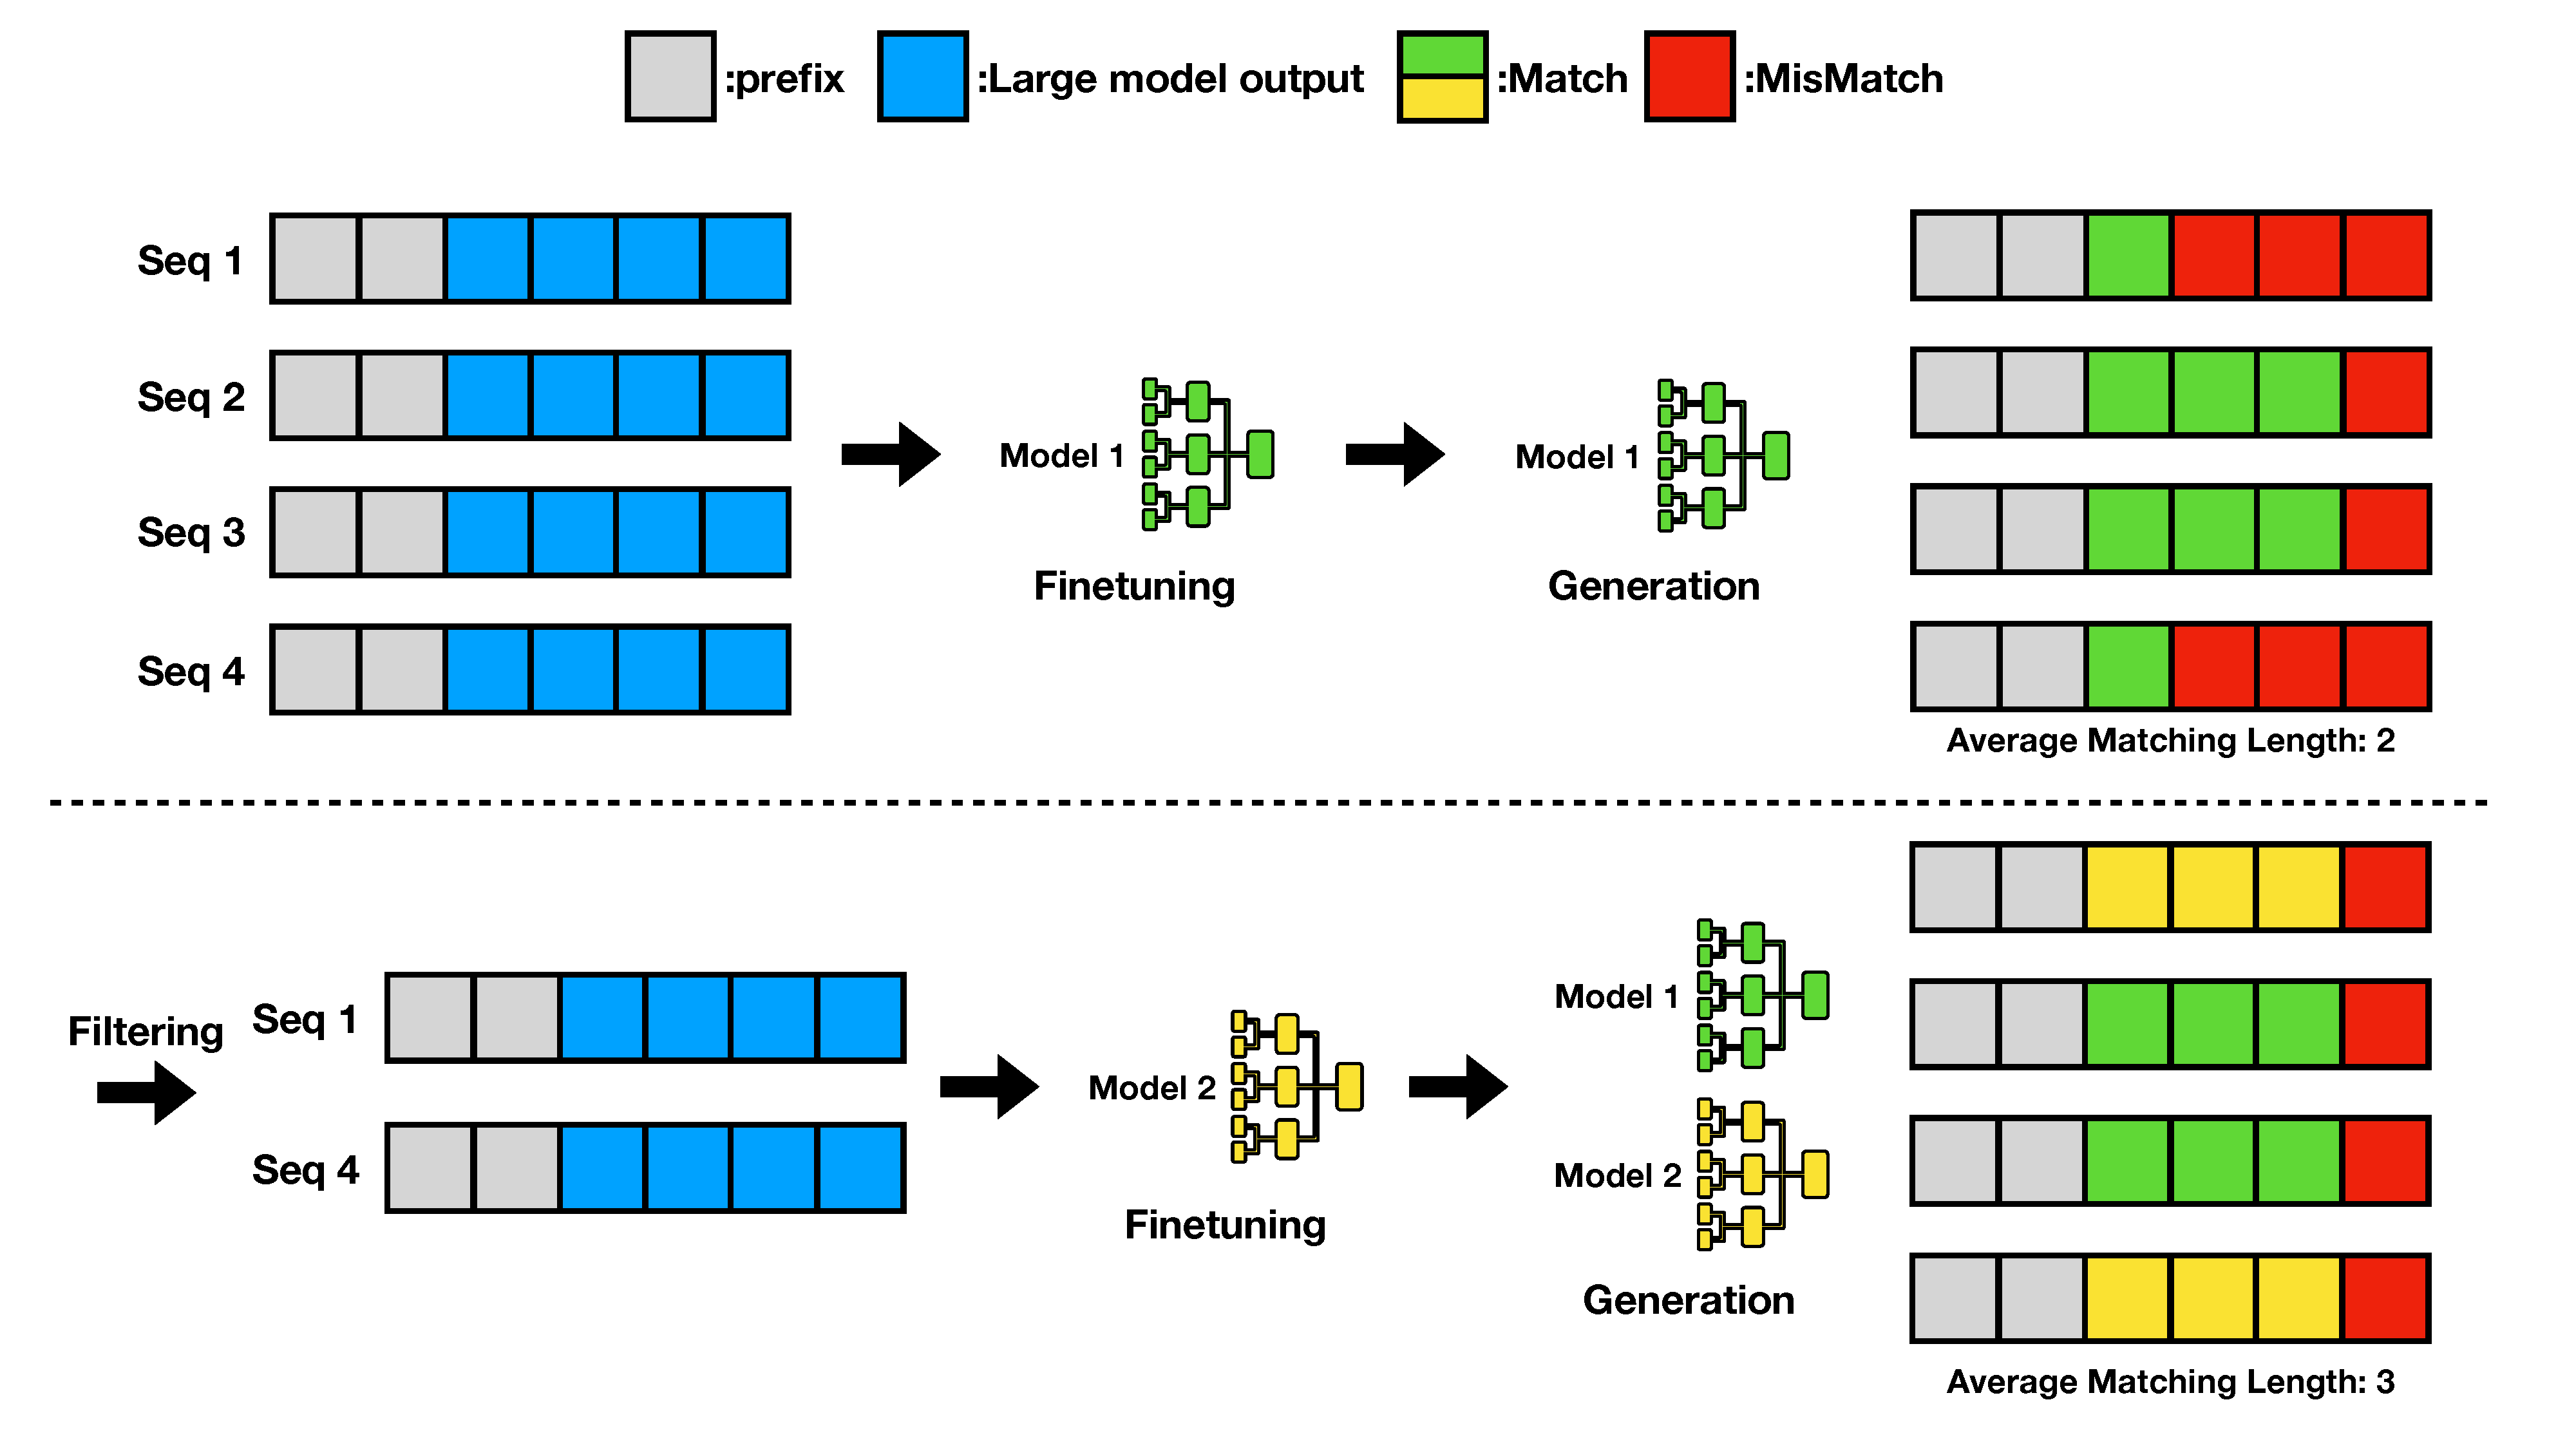
\includegraphics[scale=0.2]{figs/AdaptiveFinetuning.pdf}
    \caption{The process of Collective Boost-Tuning: with only model 1, an average matching length of 2.0 is achieved due to in-accurate alignment between model 1 and the LLM on Seq 1 and 4. However, we can improve the average matching length to 3.0 by adding model 2 which is tuned on Seq 1 and 4.\XM{(Done, to be checked)}}
    \label{fig:CBT}
\end{figure}
\fi 

\if 0
\begin{figure}
    \centering
    %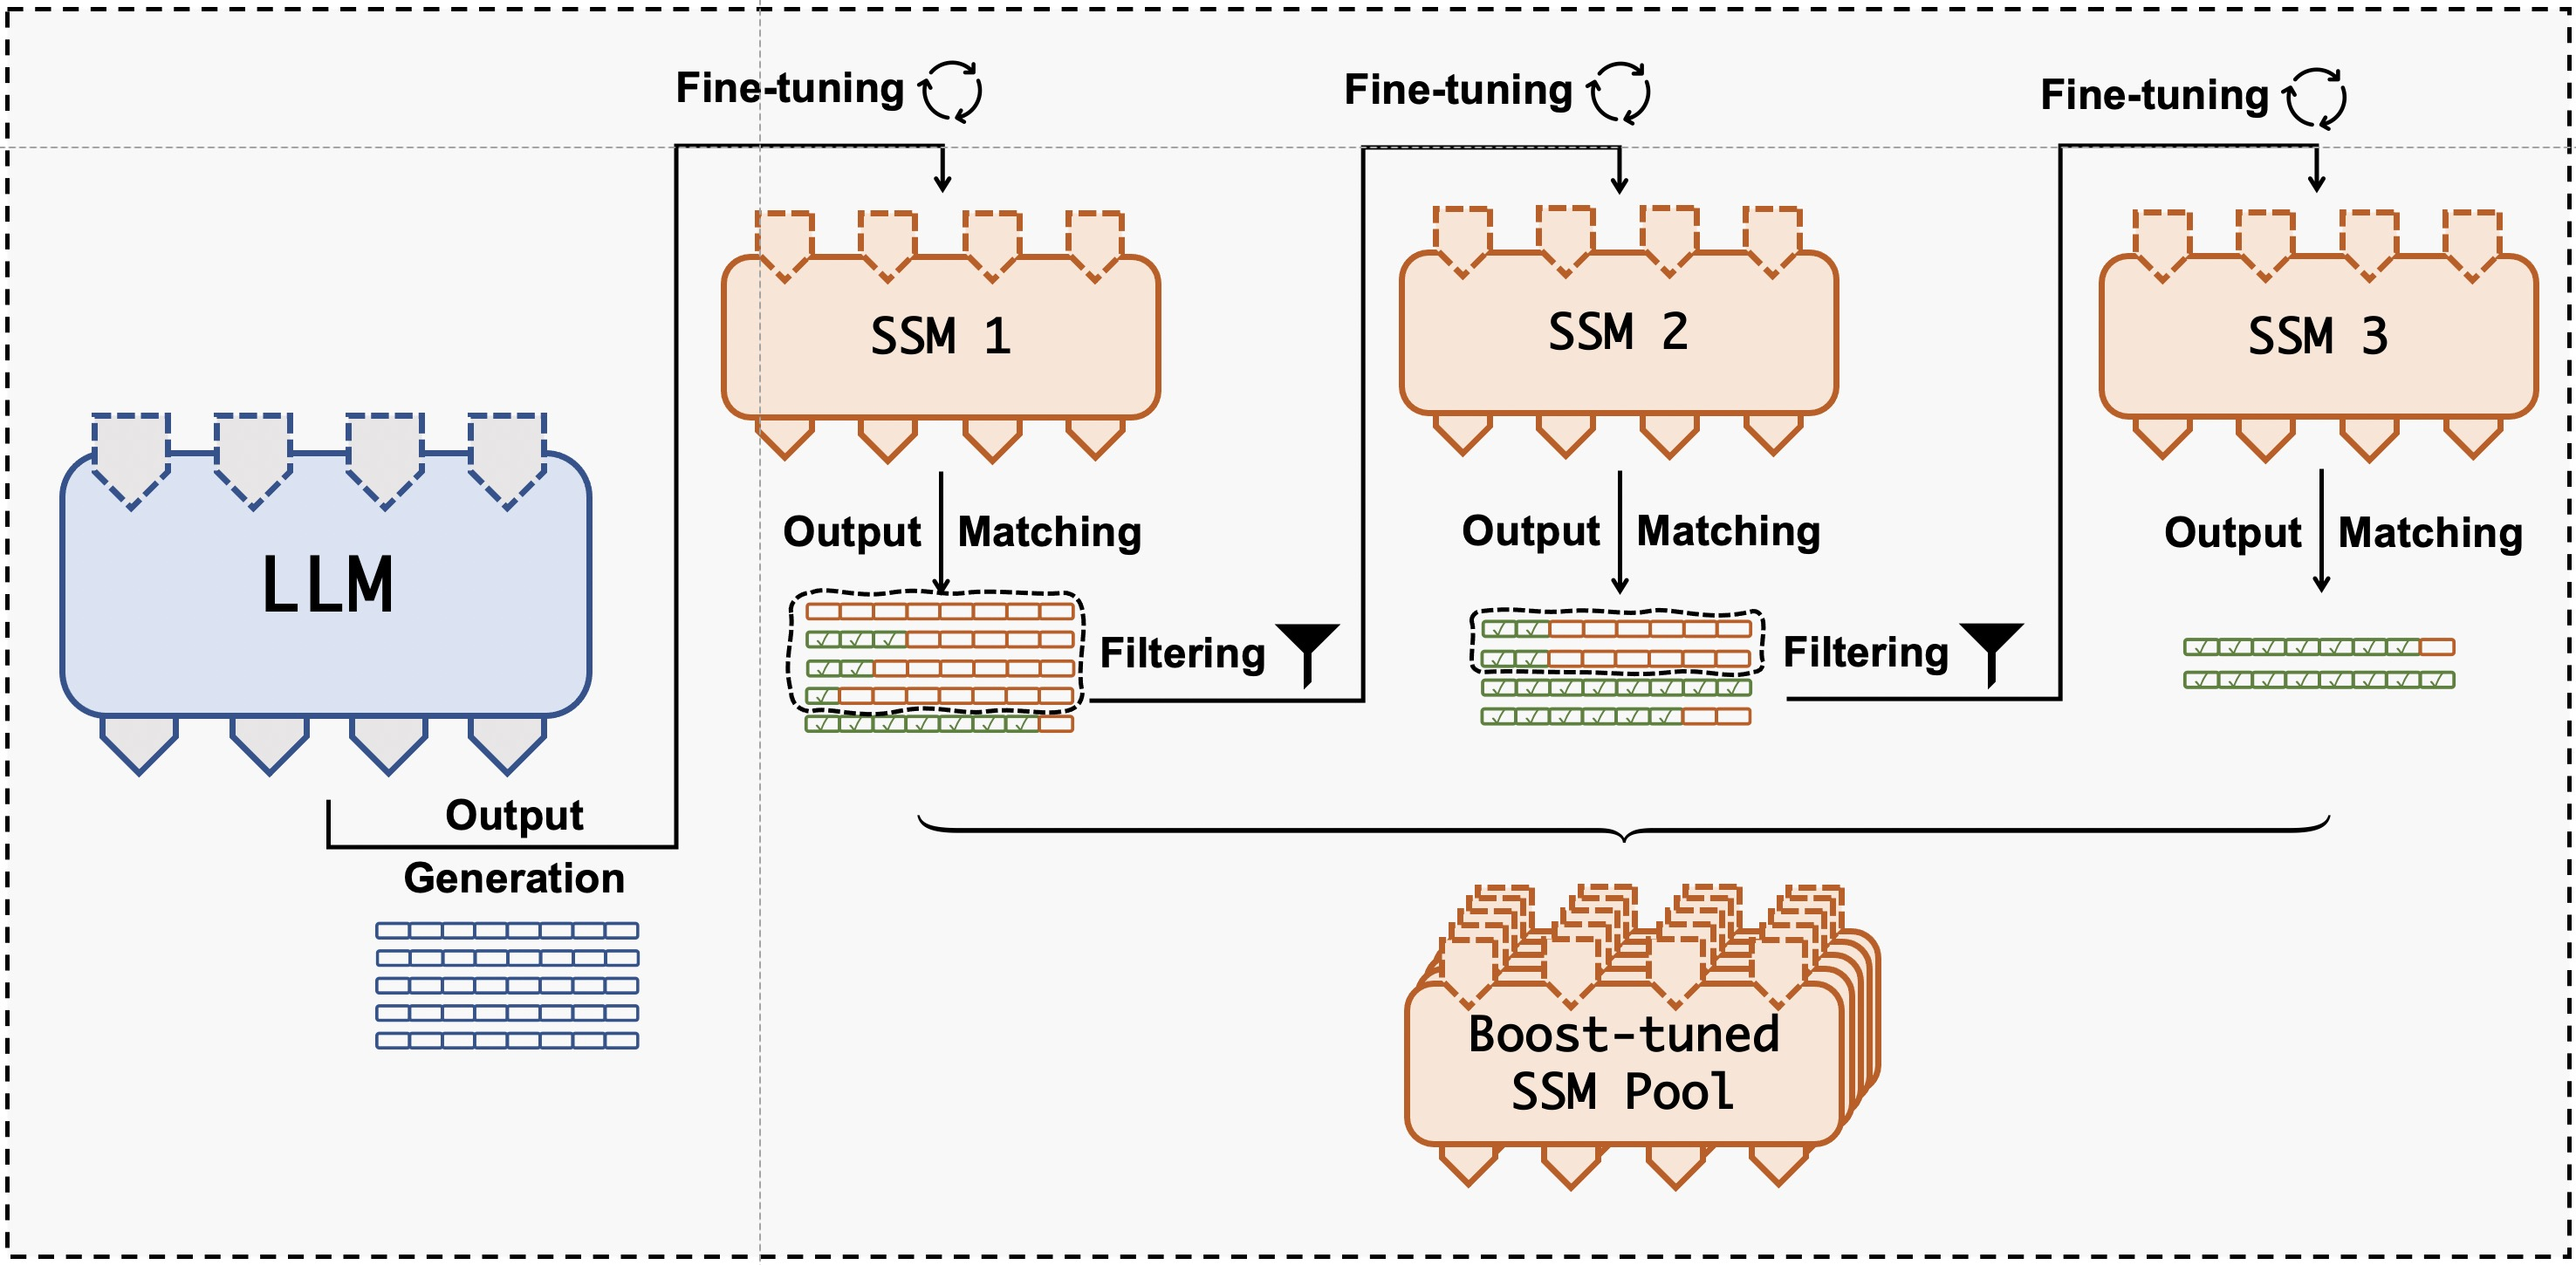
\includegraphics[scale=0.12]{figs/boost_tuning2.jpg}
    %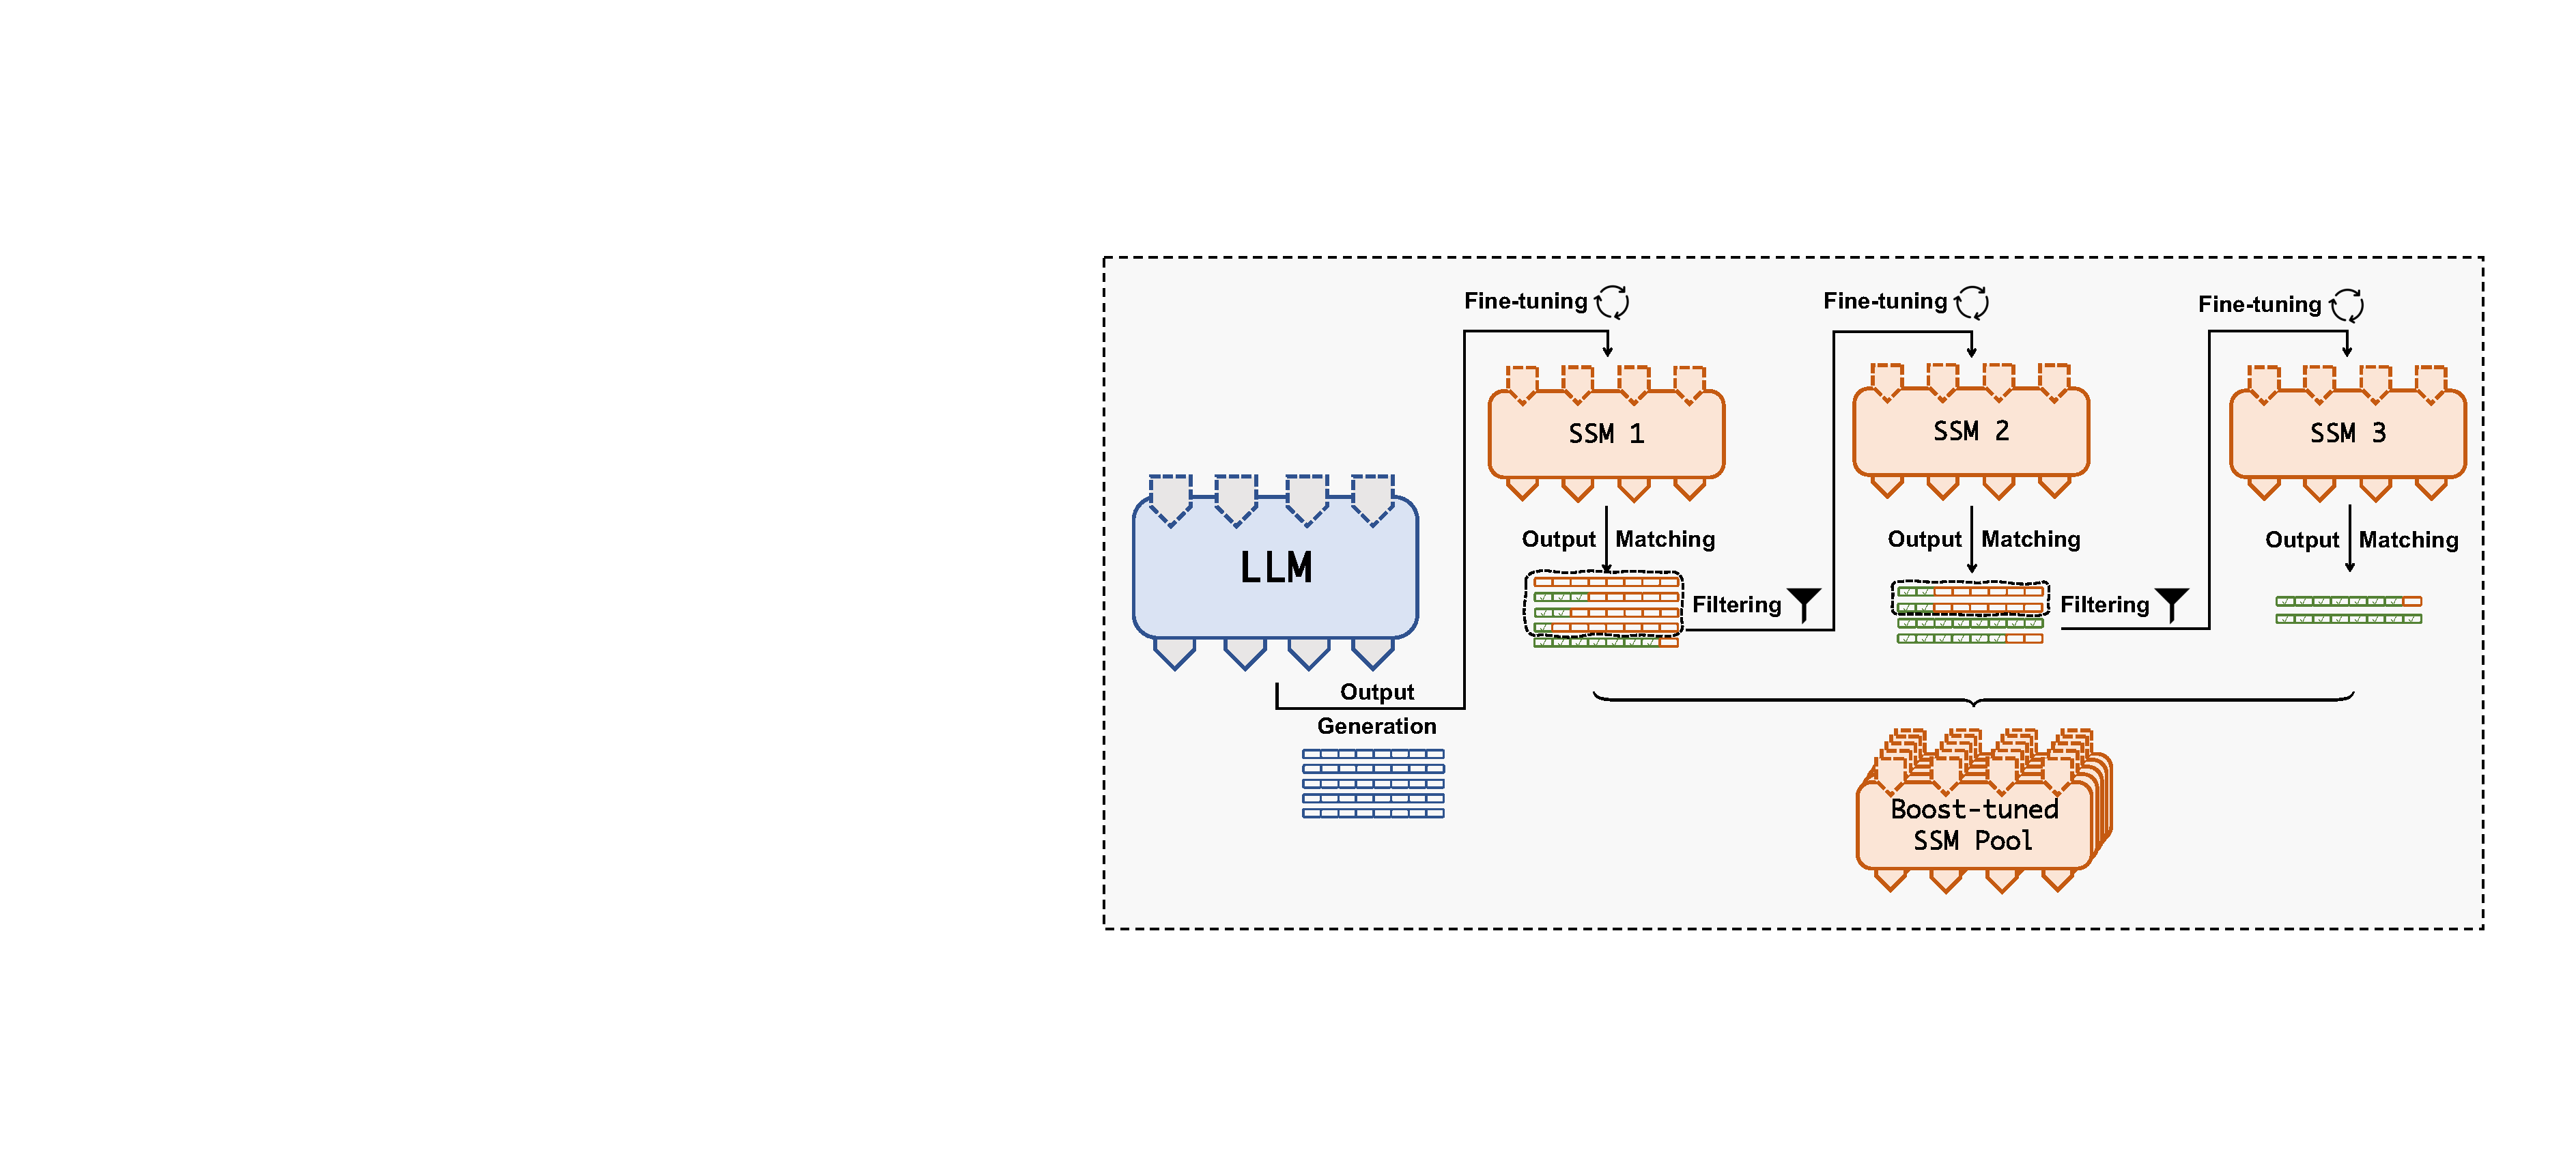
\includegraphics[scale=0.36]{figs/boost_tuning2.pdf}
    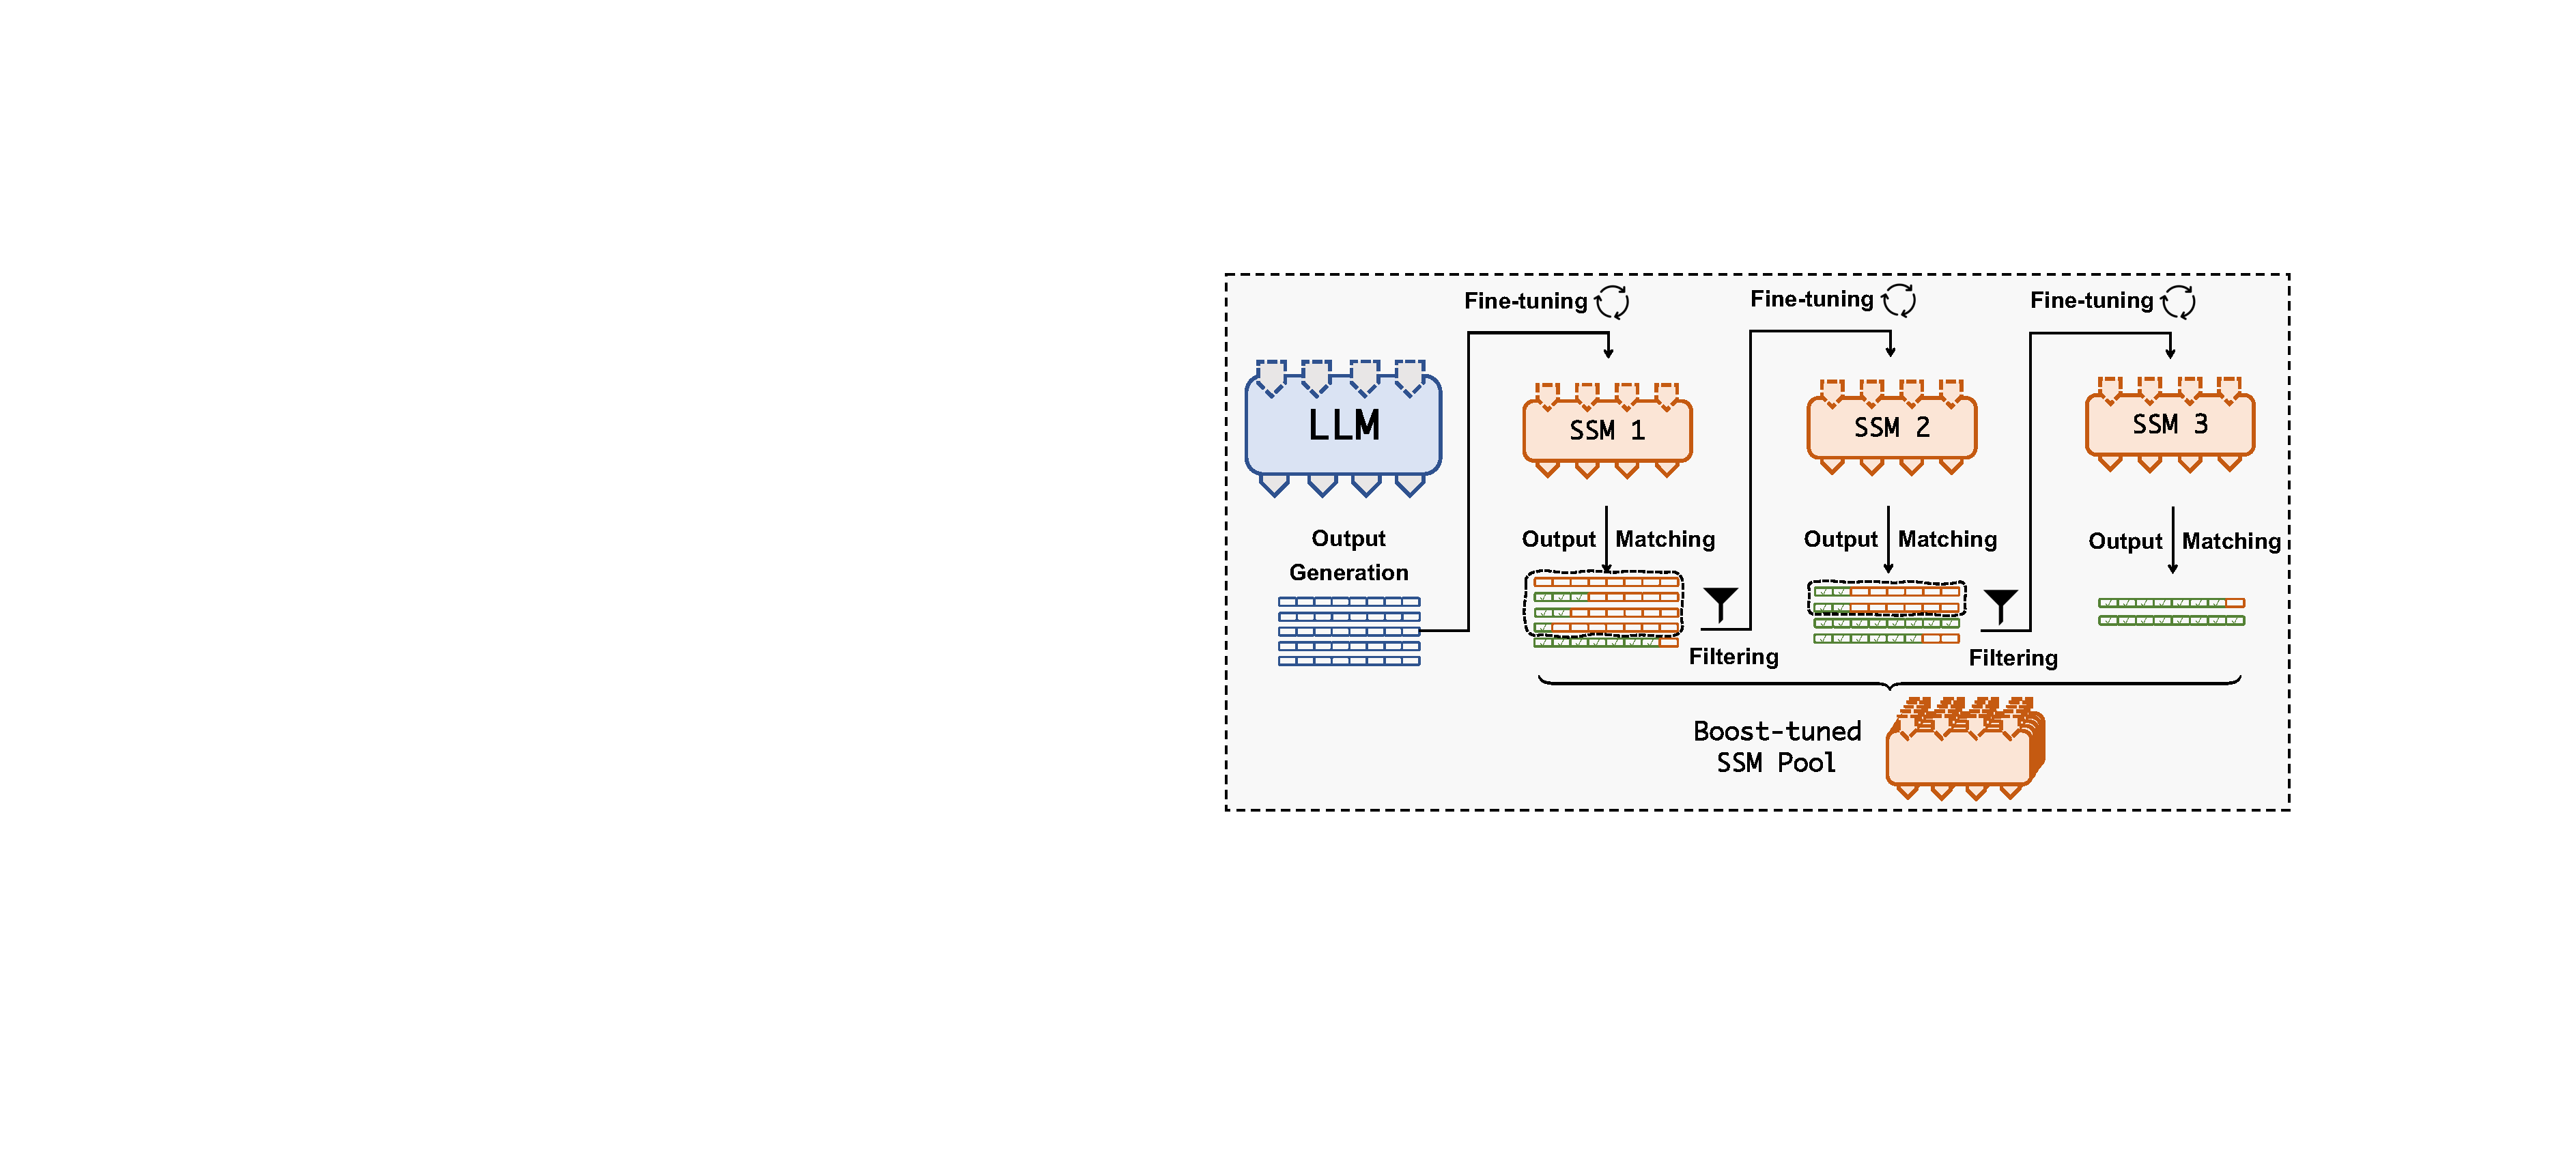
\includegraphics[scale=0.32]{figs/boost_tuning3.pdf}
    \caption{\ZJ{To be removed:} Illustrating \Sys's collective boost-tuning technique. When using a single SSM to generate token trees, \Sys can verify 2.6 tokens on average in each LLM decoding step. This is due to the misalignment between an SSM and LLM on the first four token sequences. By collectively boost-tuning three SSMs, the average number of verified tokens per LLM decoding step is improved to 7.2.}
    \label{fig:CBT}
\end{figure}
\fi

\if 0
\subsection{Learning-based Speculative Scheduler}
\label{sec:LSS}
\ZJ{To be removed.}
To discover an optimal configuration to launch multiple SSMs at each decoding step, we design a {\em learning-based} speculative scheduler that learns to decide which SSMs to use for a given input token sequence and the speculative configurations for these SSMs. 
%%%

%%%
The scheduler includes a matching length predictor and cost model. 
%%%
The matching length predictor takes as input the latest feature representation of the final hidden layer from the LLM and outputs a vector of continuous numbers, each corresponding to the expected matching length under a specific speculative configuration. 
%%%
\Sys uses a three-layer MLP as the neural architecture of the matching length predictor and considers a configuration space of beam search for each SSM, where the beam width $b \in [1, 2, 4]$ and the beam depth $d \in [1, 2, 4, 8, 16]$, therefore the MLP outputs a vector of 15 numbers, each representing the predicted matching length for a speculative configuration.
%%%
The predictor is also trained on publicly available datasets in an offload fashion.
%%%
Note that obtaining the input feature vector for the predictor does not involve extra cost as it's self-contained in the \Sys's verifier (see \Cref{sec:verification}).
%Also, notice that we don't need to pay extra effort to obtain the hidden feature since it's self-contained in the verification engine.
%%%

%%%
To achieve a higher matching length per unit of time, we define the following cost function:
\begin{equation}
    cost(b, d \mid h) = \frac{f(b, d \mid h)}{L_{\text{verify}}(b, d) + L_{\text{speculate}}(b, d) },
    \label{eqn:cost_function}
\end{equation}
where $b$ and $d$ are the beam search width and depth, $h$ is the input feature vector to the predictor, and $f(b, d \mid h)$ is the predicted matching length for the given speculative configuration $(b, d)$ and current context $h$.
%%%
$L_{\text{verify}}(b, d)$ and $L_{\text{speculate}}(b, d)$ are the estimated inference latency for the verifier and speculator, respectively, which are measured by profiling the \Sys runtime system.
%%%
Using the cost function defined in \Cref{eqn:cost_function}, \Sys chooses the configuration that minimizes the expected cost for each SSM:
\begin{equation}
    (b, d) = \arg\max_{(b, d)} cost(b, d \mid h)
\end{equation}
\fi

\section{Token Tree Verifier}
\label{sec:verification}

\if 0 
\begin{figure}
    \centering
    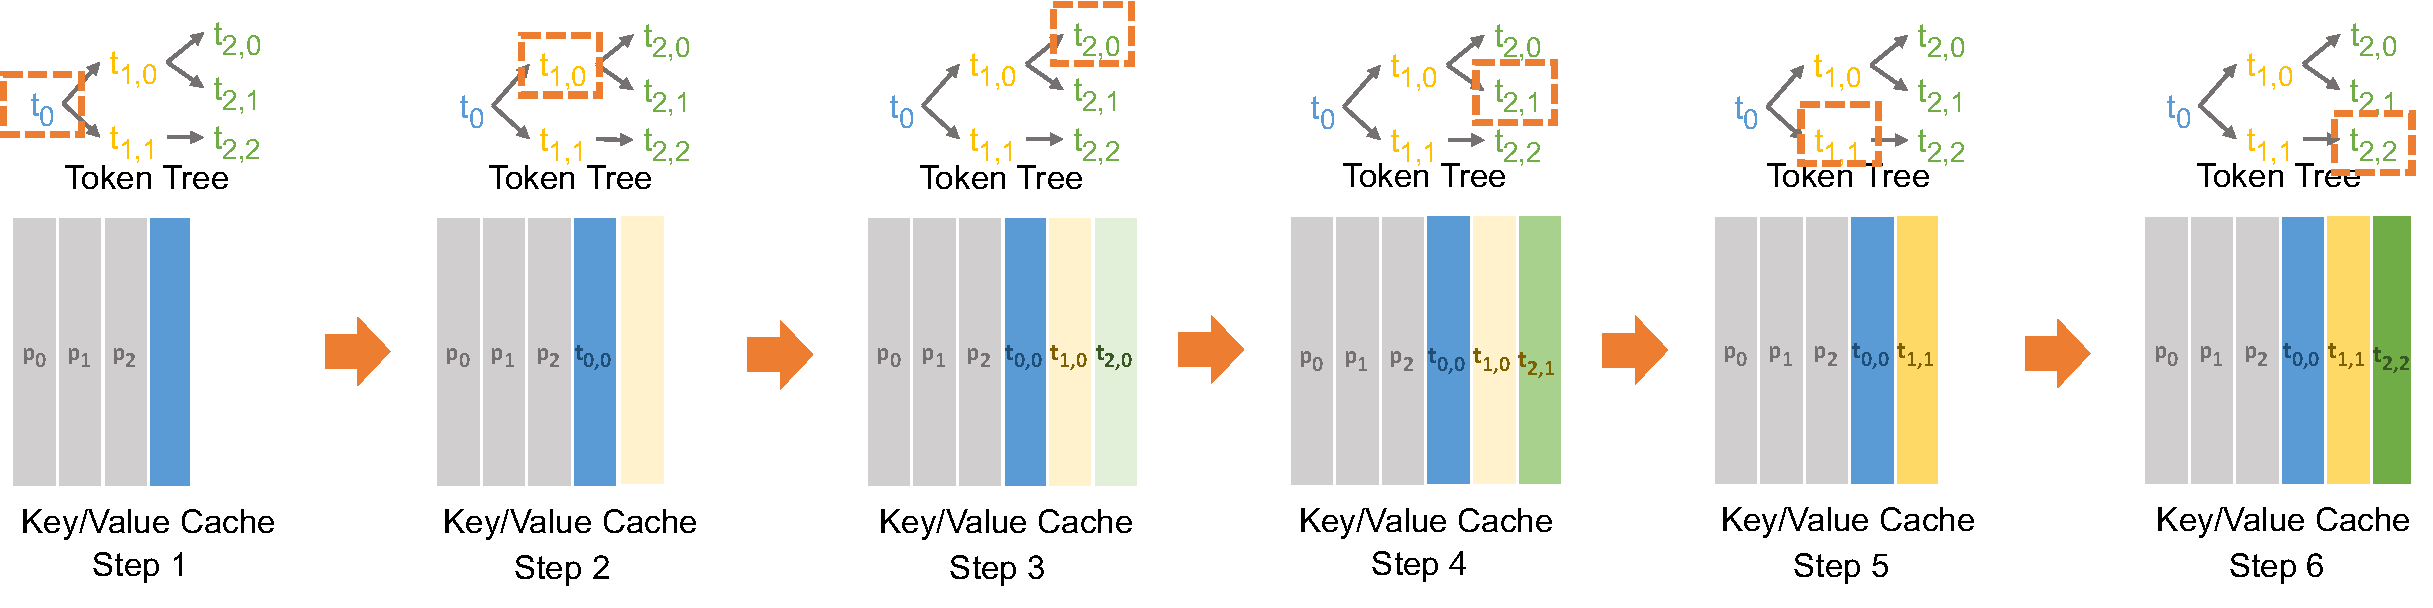
\includegraphics[scale=0.33]{figs/kv_cache_v3.pdf}
    \caption{\Sys's depth-first search mechanism to traverse a token tree.\XM{Working on this figure (Done, To be replaced)}}
    \label{fig:kv_cache}
\end{figure}
\fi

\begin{figure}
    \centering
    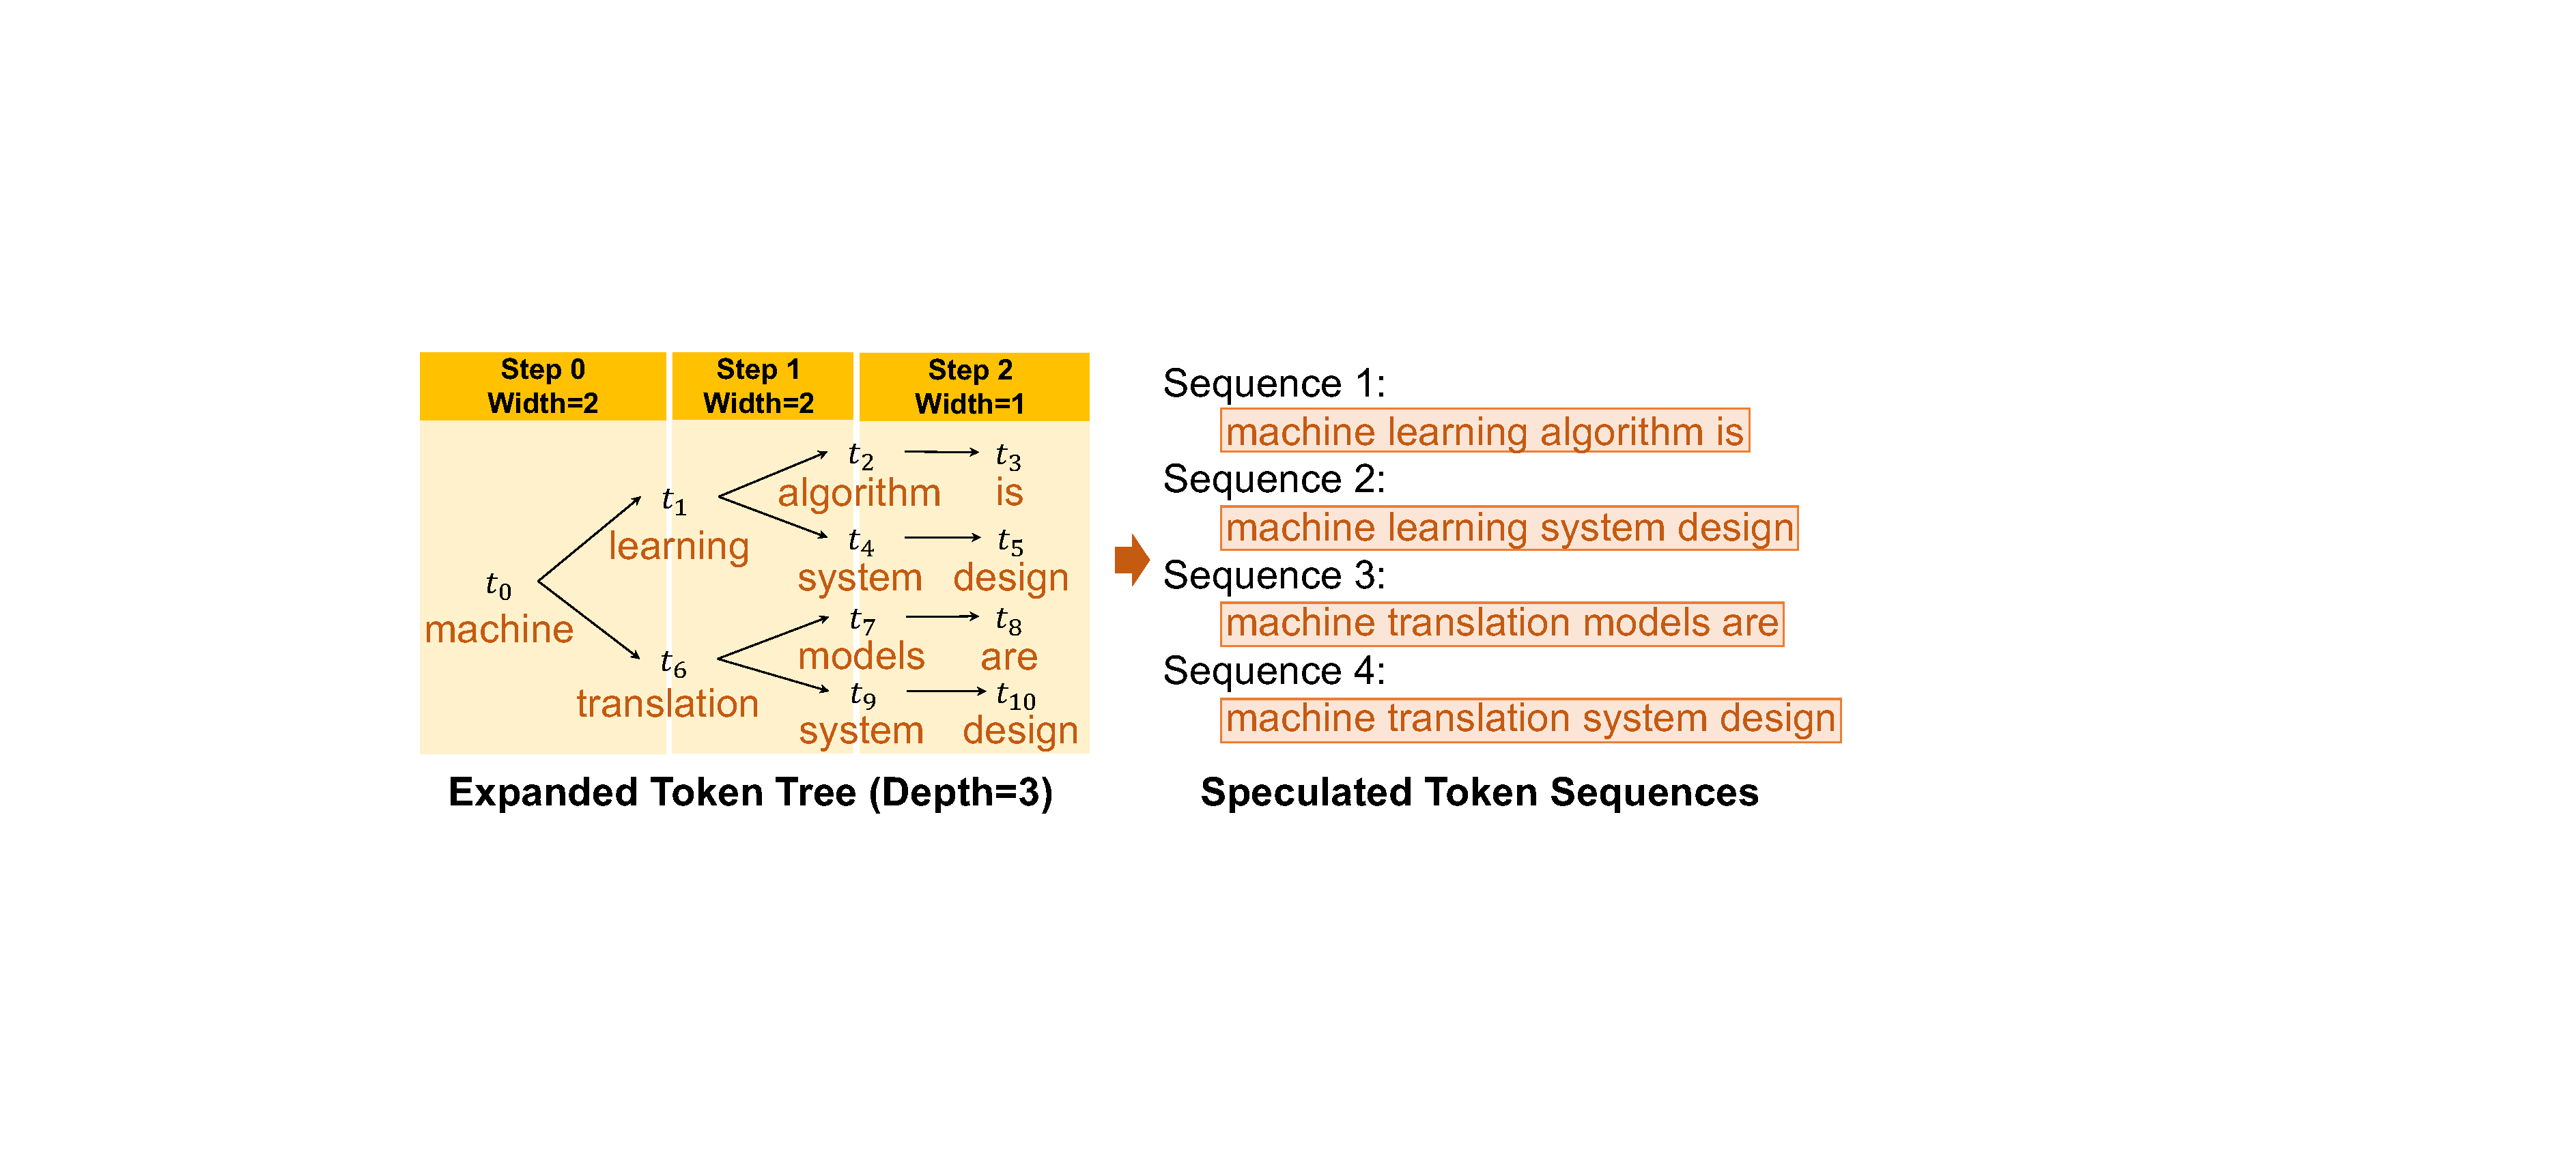
\includegraphics[width=\linewidth]{rebuttal_figs/token_tree3.pdf}
    \caption{\rev{Illustration of token tree expansion.}}
    % \ZJ{Fonts too small. Consider increasing the font size if possible.}
%     \caption{
% Merging three sequences of tokens (left) into a token tree (right), whose node each identifies a token sequence. For example, node $t_4$ represents a token sequence $[t_0, t_1, t_3, t_4]$ that translates to ``machine learning system design''.
% \XM{Working on this}}
    \label{fig:token_tree_merge}
\end{figure}

This section introduces \sys's {\em token tree verifier}, which takes as input a token tree generated by the speculator and verifies the correctness of its tokens against an LLM's output.
%
A key idea behind the design of \Sys is {\em simultaneously} verifying all sequences of a token tree against the original LLM's output by making a {\em single} pass over the LLM's parameters.
%%%
This functionality allows \Sys to opportunistically decode {\em multiple} tokens (instead of a single token in incremental decoding), resulting in reduced memory accesses to the LLM's parameters.
%%%
A challenge \Sys must address in token tree verification is efficiently computing the attention scores for {\em all} sequences of a token tree.
%%%
To this end, we introduce {\em tree attention}, which generalizes the attention mechanism~\cite{vaswani2017attention} from sequence to tree structure.
In addition, we develop a {\em tree-based parallel decoding} mechanism that can decode {\em all} tokens in a token tree in parallel.
%\Sys performs {\em tree attention}, a fast and cheap approach to performing Transformer-based attention computation for a token tree, and a number of important system-level optimizations to address this challenge.

\S\ref{subsec:tree_attention} and \S\ref{subsec:optimization} describe tree attention and tree-based parallel decoding. 
\S\ref{subsec:verification} introduces the mechanism to verify a token tree against the LLM's output.
%\Cref{subsec:verification} introduces the mechanism \Sys uses to verify a token tree against an LLM, and \Cref{subsec:optimization} presents \Sys's optimizations to accelerate token tree verification.

\if 0
\ZJ{TO BE REMOVED <---}
\begin{definition}[Token Tree]
A token tree $\m{N}$ is a tree structure, where each node $u \in \m{N}$ is labelled with a token $t_u$, and $p_u$ represents $u$'s parent node in the token tree. 
For each node $u$, $S_u$ represents a sequence of tokens identified by concatenating $S_{p_u}$ and $\{t_u\}$\footnote{For the root node $r$, $S_r$ represents the token sequence $\{t_r\}$.}.
\end{definition}

\Sys uses a {\em token tree} to store the results generated by the learning-based speculator. Specifically, \Sys receives multiple token sequences generated by different SSMs, each of which can be considered as a token tree (with linear tree structure), and merges them into a single token tree.

\begin{definition}[Token Tree Merge]
$\m{M}$ is the tree merge of $m$ token trees $\{\m{N}_i\}$ ($1\leq i \leq m$) if and only if $\forall 1\leq i \leq m, \forall u \in \m{N}_i, \exists v \in \m{M}$ such that $S_v = S_u$ and vice versa.
\end{definition}

Intuitively, each token tree represents a set of token sequences. Merging multiple token trees produces a new tree that includes all token sequences of the original trees.
For example, \Cref{fig:token_tree_merge} shows the token tree derived by merging three sequences of tokens.
Each token sequence is identified by a node in the merged token tree.
%and performs tree merge to produce a speculated token tree. Each token sequence can be considered as a special token tree. For $m$ input token trees $\{\m{N}_i\}$ ($1 \leq i \leq m$), $N$ is the output of 
\ZJ{--->TO BE REMOVED}
\fi 

\subsection{Tree Attention}
\label{subsec:tree_attention}
Transformer-based language models use the attention mechanism to reason about sequential information~\cite{vaswani2017attention}.
LLMs generally use decoder-only, multi-head self-attention, which takes a single input tensor $X$ and computes an output tensor $O$ via scaled multiplicative formulations as follows.
\begin{eqnarray}
    Q_i = X \times W_i^Q, & K_i = X \times W_i^K, \\
    V_i = X \times W_i^V, & A_i = \frac{(Q_i \times K_i^T)}{\sqrt{d}}, \\
    H_i = \textrm{softmax}\big(\textrm{mask}(A_i)\big) V_i, & O = (H_1, ...,H_h) W^O 
    \label{eqn2}
\end{eqnarray}
where $Q_i$, $K_i$, and $V_i$ denote the query, key, and value tensors of the $i$-th attention head ($1\leq i \leq h$), $W_i^Q$, $W_i^K$, and $W_i^V$ are the corresponding weight matrices. 
$A_i$ is an $l\times l$ matrix that represents the attention scores between different tokens in the input sequence, where $l$ is the sequence length. To preserve causality when generating tokens (i.e., a token in the sequence should not affect the hidden states of any preceding tokens), the following causal mask function is applied:
\begin{equation}
    \textrm{mask}(A)_{jk} =     \begin{cases}
    A_{jk} & j \geq k\\
    - \infty & j < k 
    \end{cases}.
\end{equation}
Intuitively, when computing the attention output of the $j$-th token in the sequence, all subsequent tokens should have an attention score of $-\infty$ to indicate that the subsequent tokens will not affect the attention output of the $j$-th token\footnote{Note that we use $-\infty$ (instead of 0) to guarantee that the softmax's output is 0 for these positions.}. 
%%%
In Equation~\ref{eqn2}, $H_i$ represents the output of the $i$-th attention head, and $W_O$ is a weight matrix used for computing the final output of the attention layer.

Note that the attention mechanism described above applies only to a sequence of tokens. We generalize the attention mechanism to arbitrary tree structures.
%For each node $u$ in a token tree, its tree attention is defined as the output of computing original attention on $S_u$ (i.e., the token sequence represented by $u$). 

\begin{definition}[Tree Attention]
For a token tree $\m{N}$ and an arbitrary node $u \in \m{N}$, its tree attention is defined as the output of computing the original Transformer-based sequence attention on $S_u$ (i.e., the token sequence represented by $u$):
\begin{equation}
    \textproc{TreeAttention}(u) = \textproc{Attention}(S_u) \forall u \in \m{N}
\end{equation}
\end{definition}
For a given set of token sequences, since each sequence $S$ is covered by a node of the merged token tree, performing tree attention on the token tree allows \Sys to obtain the attention output for {\em all} token sequences. 
% Note that the semantic of \Sys's tree attention is different from prior tree-structured attention work~\cite{Nguyen2020}, which we discuss in \Cref{sec:related}.


\subsection{Tree-based Parallel Decoding}
\label{subsec:optimization}

\begin{figure*}
    \centering
    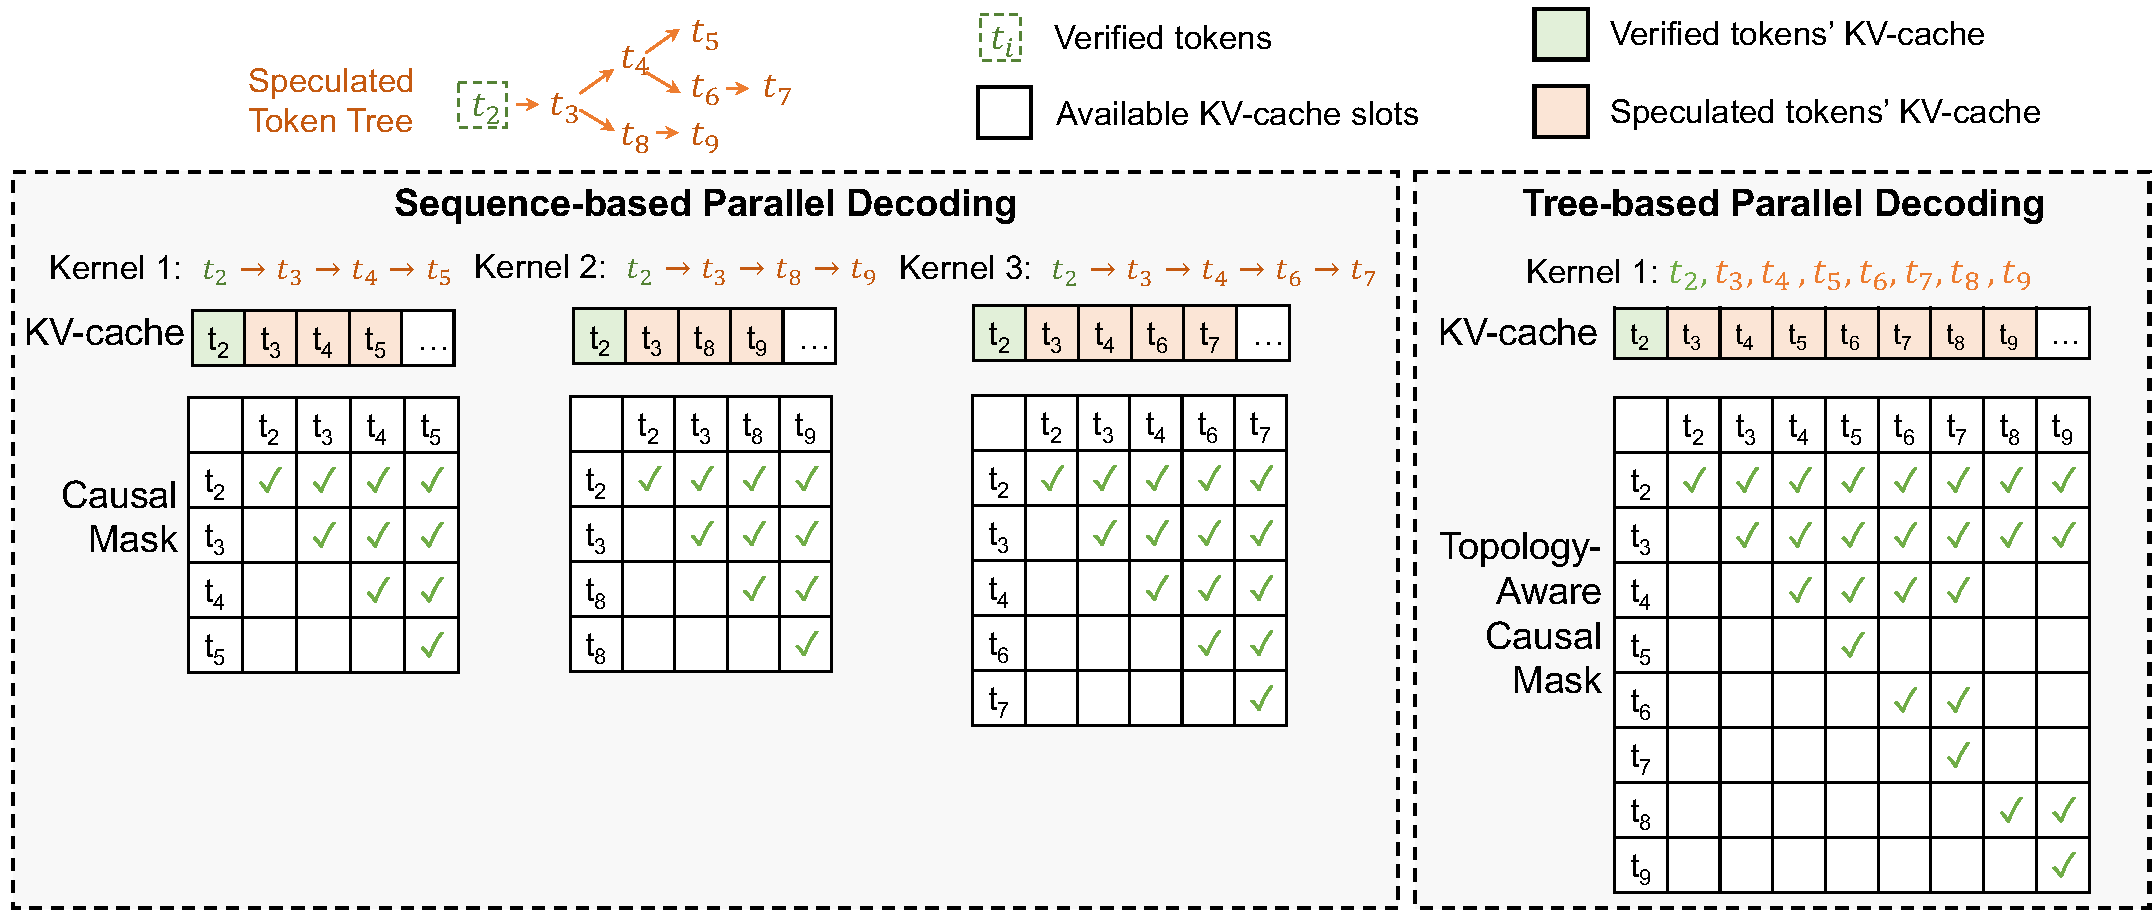
\includegraphics[width=0.9\textwidth]{figs/new_kv_cache2.pdf}
    \caption{Comparing \Sys's tree-based parallel decoding with existing sequence-based decoding.}
    \label{fig:kv_cache}
\end{figure*}

This section describes \sys's {\em tree-based parallel decoding} mechanism for computing tree attention for {\em all} tokens in a token tree {\em in parallel}.
A key challenge \Sys must address in computing tree attention is managing {\em key-value cache}. 
%%%
In particular, the attention mechanism of Transformer~\cite{vaswani2017attention} requires accessing the keys and values of all preceding tokens to compute the attention output of each new token, as shown in Equation~\ref{eqn2}.
%%%
To avoid recomputing these keys and values, today's LLM inference systems generally cache the keys and values of all tokens for reuse in future iterations, since the causal relation guarantees that a token's key and value remain unchanged in subsequent iterations (i.e., $\rm{mask(A)_{jk}} = -\infty$ for any $j < k$).
%%% 
However, when computing tree attention, different sequences in a token tree may include conflicting key-value caches. For example, for the speculated token tree in \Cref{fig:kv_cache}, two token sequences $(t_2, t_3, t_4, t_5)$ and $(t_2, t_3, t_8, t_9)$ have different keys and values for the third and fourth positions.

A straightforward approach to supporting key-value cache is employing the sequence-based decoding of existing LLM inference systems and using a different key-value cache for each sequence of a token tree, as shown on the left of \Cref{fig:kv_cache}.
However, this approach is computationally very expensive and involves redundant computation, since two token sequences sharing a common prefix have the same attention outputs for the common prefix due to the causal mask in Equation~\ref{eqn2}.
In addition, launching one kernel for each token sequence introduces additional kernel launch overhead.

\Sys introduces two key techniques to realize tree-based parallel decoding.

\paragraph{Depth-first search to update key-value cache.} Instead of caching the keys and values for individual token sequences of a token tree, \Sys reuses the same key-value cache across all token sequences by leveraging a {\em depth-first search} mechanism to traverse the token tree, as shown in \Cref{fig:kv_cache}, where \Sys visits $t_2,t_3,...,t_9$ by following a depth-first order to traverse the token tree and update the shared key-value cache.
%%%
This approach allows \Sys to maintain the correct keys and values for all preceding tokens when computing the attention output of a new token.

\paragraph{Topology-aware causal mask.} A straightforward approach to computing tree attention is calculating the tree attention output for individual tokens by following the depth-first order described earlier. 
However, this approach would result in high GPU kernel launch overhead since each kernel only computes tree attention for one token sequence.
In addition, executing these kernels in parallel requires additional GPU memory to store their key-value caches separately due to cache conflict.
%%%
A key challenge that prevents \Sys from batching multiple tokens is that the attention computation for different tokens requires different key-value caches and therefore cannot be processed in parallel.

We introduce {\em topology-aware casual mask} to fuse tree attention computation of all tokens in a single kernel. 
To batch attention computation, \Sys uses a tree topology instead of the original sequence topology to store the keys and values of all tokens in a token tree in the key-value cache.
%the key-value cache of all speculated tokens of a token tree when computing attention scores.
For example, to compute tree attention for the speculated token tree shown in \Cref{fig:kv_cache}, \Sys takes both verified tokens (i.e., $t_2$) and all speculated tokens (i.e., $t_3,t_4,...,t_9$) as inputs.
This approach allows \Sys to fuse the attention computation into a single kernel but also results in attention scores that violate the causal dependency (e.g., $t_7$'s attention computation uses all previous tokens, including $t_5$ which is not in $t_7$'s token sequence).
To fix the attention scores for these pairs, \Sys updates the causal mask based on the token tree's topology.
This approach computes the exact same attention output as incremental decoding, while resulting in much fewer kernel launches compared to sequence-based decoding.

\if 0 

\section*{Old version}
This section describes \sys's {\em tree-based parallel decoding} algorithm for computing tree attention for {\em all} tokens in a token tree {\em in parallel}.
A straightforward approach to computing tree attention is directly computing the original sequence-based attention for all token sequences (i.e., $\textproc{Attention}(S_u$) for all $u\in\m{N}$).
However, this approach is computationally very expensive and involves redundant computation, since two token sequences sharing a common prefix have the same attention outputs for the common prefix due to the causal mask in Equation~\ref{eqn2}.

\paragraph{Depth-first search to update key-value cache.} As shown in Equation~\ref{eqn2}, the attention mechanism of Transformer~\cite{vaswani2017attention} requires accessing the keys and values of all preceding tokens to compute the attention output of each new token.
To avoid recomputing these keys and values, today's LLM inference systems generally cache the keys and values of all tokens for reuse in future iterations, since the causal relation guarantees that a token's key and value remain unchanged in subsequent iterations (i.e., $\rm{mask(A)_{jk}} = -\infty$ for any $k > j$).

A key challenge \Sys must address in verifying a token tree is that different sequences in the token tree may include conflicting key-value caches. For the speculated token tree at the top of \Cref{fig:kv_cache}, two token sequences $(t_2, t_3, t_4, t_5)$ and $(t_2, t_3, t_8, t_9)$ have different keys and values for the third and fourth positions.
%%%
A straightforward approach to supporting key-value cache is employing the sequence-based decoding of existing LLM inference systems and having a different key-value cache for each sequence of a token tree, as shown in the top-left of \Cref{fig:kv_cache}.
%%%
However, this approach requires multiple replicas of key-value caches for verifying different sequences and introduces redundant computations since sequences in a token tree may share common prefixes.

Instead of caching the keys and values for individual token sequences of a token tree, \Sys reuses the same key-value cache across all token sequences by leveraging a {\em depth-first search} mechanism to traverse the token tree, as shown in the top-right of \Cref{fig:kv_cache}, where the arrows indicate how the key-value cache is updated when decoding different tokens.
%%%
By following a depth-first order to traverse the token tree and update the shared key-value cache, \Sys is able to maintain the correct keys and values for all preceding tokens when computing the attention output of a new token. 

\paragraph{Tree-based parallel decoding.} Existing LLM inference systems use an incremental decoding approach that decodes a single token in each iteration during the generative phase. 
%%%
Therefore, a similar approach for computing tree attention is iteratively calculating the attention output for individual tokens in the token tree by following the depth-first order described earlier.
%using a depth-first order to traverse the token tree and computing the attention score for one token in each iteration.
%%%
However, this approach would result in high GPU kernel launch overhead since each kernel only computes tree attention for a single token.
%%%
A key challenge that prevents \Sys from batching multiple tokens is that the attention computation for different tokens requires different key-value caches and therefore cannot be processed in parallel.
For example, the token-based decoding in \Cref{fig:kv_cache} shows the key-value caches needed for each token.

\Sys uses a {\em tree-based parallel decoding} algorithm to opportunistically batch multiple tokens in a token tree. Specifically, \Sys leverages the causal mask of generative LLM inference and groups multiple tokens into a single kernel if each token is the subsequent token's parent.
%%%
For example, a depth-first search to traverse the token tree in \Cref{fig:kv_cache} is $(t_3, t_4, t_5, t_6, t_7, t_8, t_9)$. Instead of launching 7 individual kernels to compute the tree attention for these tokens, \Sys groups them into three kernels: $(t_3, t_4, t_5)$, $(t_6, t_7)$, and $(t_8, t_9)$, within each of which a token is a child of the previous token.
%%%
To batch attention computation, \Sys uses the key-value cache of the kernel's last token (i.e., $t_5$ for the first kernel), which results in attention scores that violate the causal dependency. \Sys then fixes the attention scores for these pairs.
%%%
This approach computes the exact same attention output as incremental decoding, while achieving much fewer kernel launches compared to the sequence and token-based decoding mechanism.
\fi 

%\paragraph{Committing tokens.}
%The depth-first order \Sys uses to traverse a token tree does not guarantee that \Sys stores correct key-value cache after the tree-based parallel decoding. 


\subsection{Token Verification}
\label{subsec:verification}

For a given speculated token tree $\m{N}$, 
%\Sys uses the tree attention mechanism described in \Cref{subsec:tree_attention} to compute an attention output for each node $u\in\m{N}$. 
%%%
%A key advantage of this approach is enabling \Sys to examine all tokens in parallel by visiting the LLM's parameters once.
%%%
\Sys uses tree-based parallel decoding (see \Cref{subsec:optimization}) to compute its tree attention and generate an output tensor $\m{O}$ that includes a token for each node $u\in\m{N}$.
%%%
Next, \Sys's {\em token tree verifier} examines the correctness of speculated tokens against the LLM. 
\Sys supports both greedy and stochastic sampling as shown in~\Cref{alg2}. 
%%%
\if 0
\textproc{Speculate} takes the current token sequence $\m{S}$ as an input and generates a speculated token tree $\m{N}$. 
% \Sys's use of an LLM is different from existing systems: the LLM takes a token tree $\m{N}$ as an input and generates a token $\m{O}(u)$ for each node $u \in \m{N}$.
The \textproc{TreeParallelDecode} function then generates all tokens in $\m{O}$ in a single LLM decoding step (see~\Cref{sec:verification}).
Finally, \textproc{VerifyGreedy} and \textproc{VerifyStochastic} examine the speculated token tree $\m{N}$ against the LLM's output $\m{O}$ and produces a sequence of verified tokens $\m{V}$ following greedy decoding or stochastic sampling respectively, which can be directly appended to the current token sequence $\m{S}$.
\fi
%%%
%Besides, \Sys further supports both greedy decoding and stochastic decoding as illustrated in~\Cref{fig:decodings} and described below.
\begin{figure}
    \centering
    %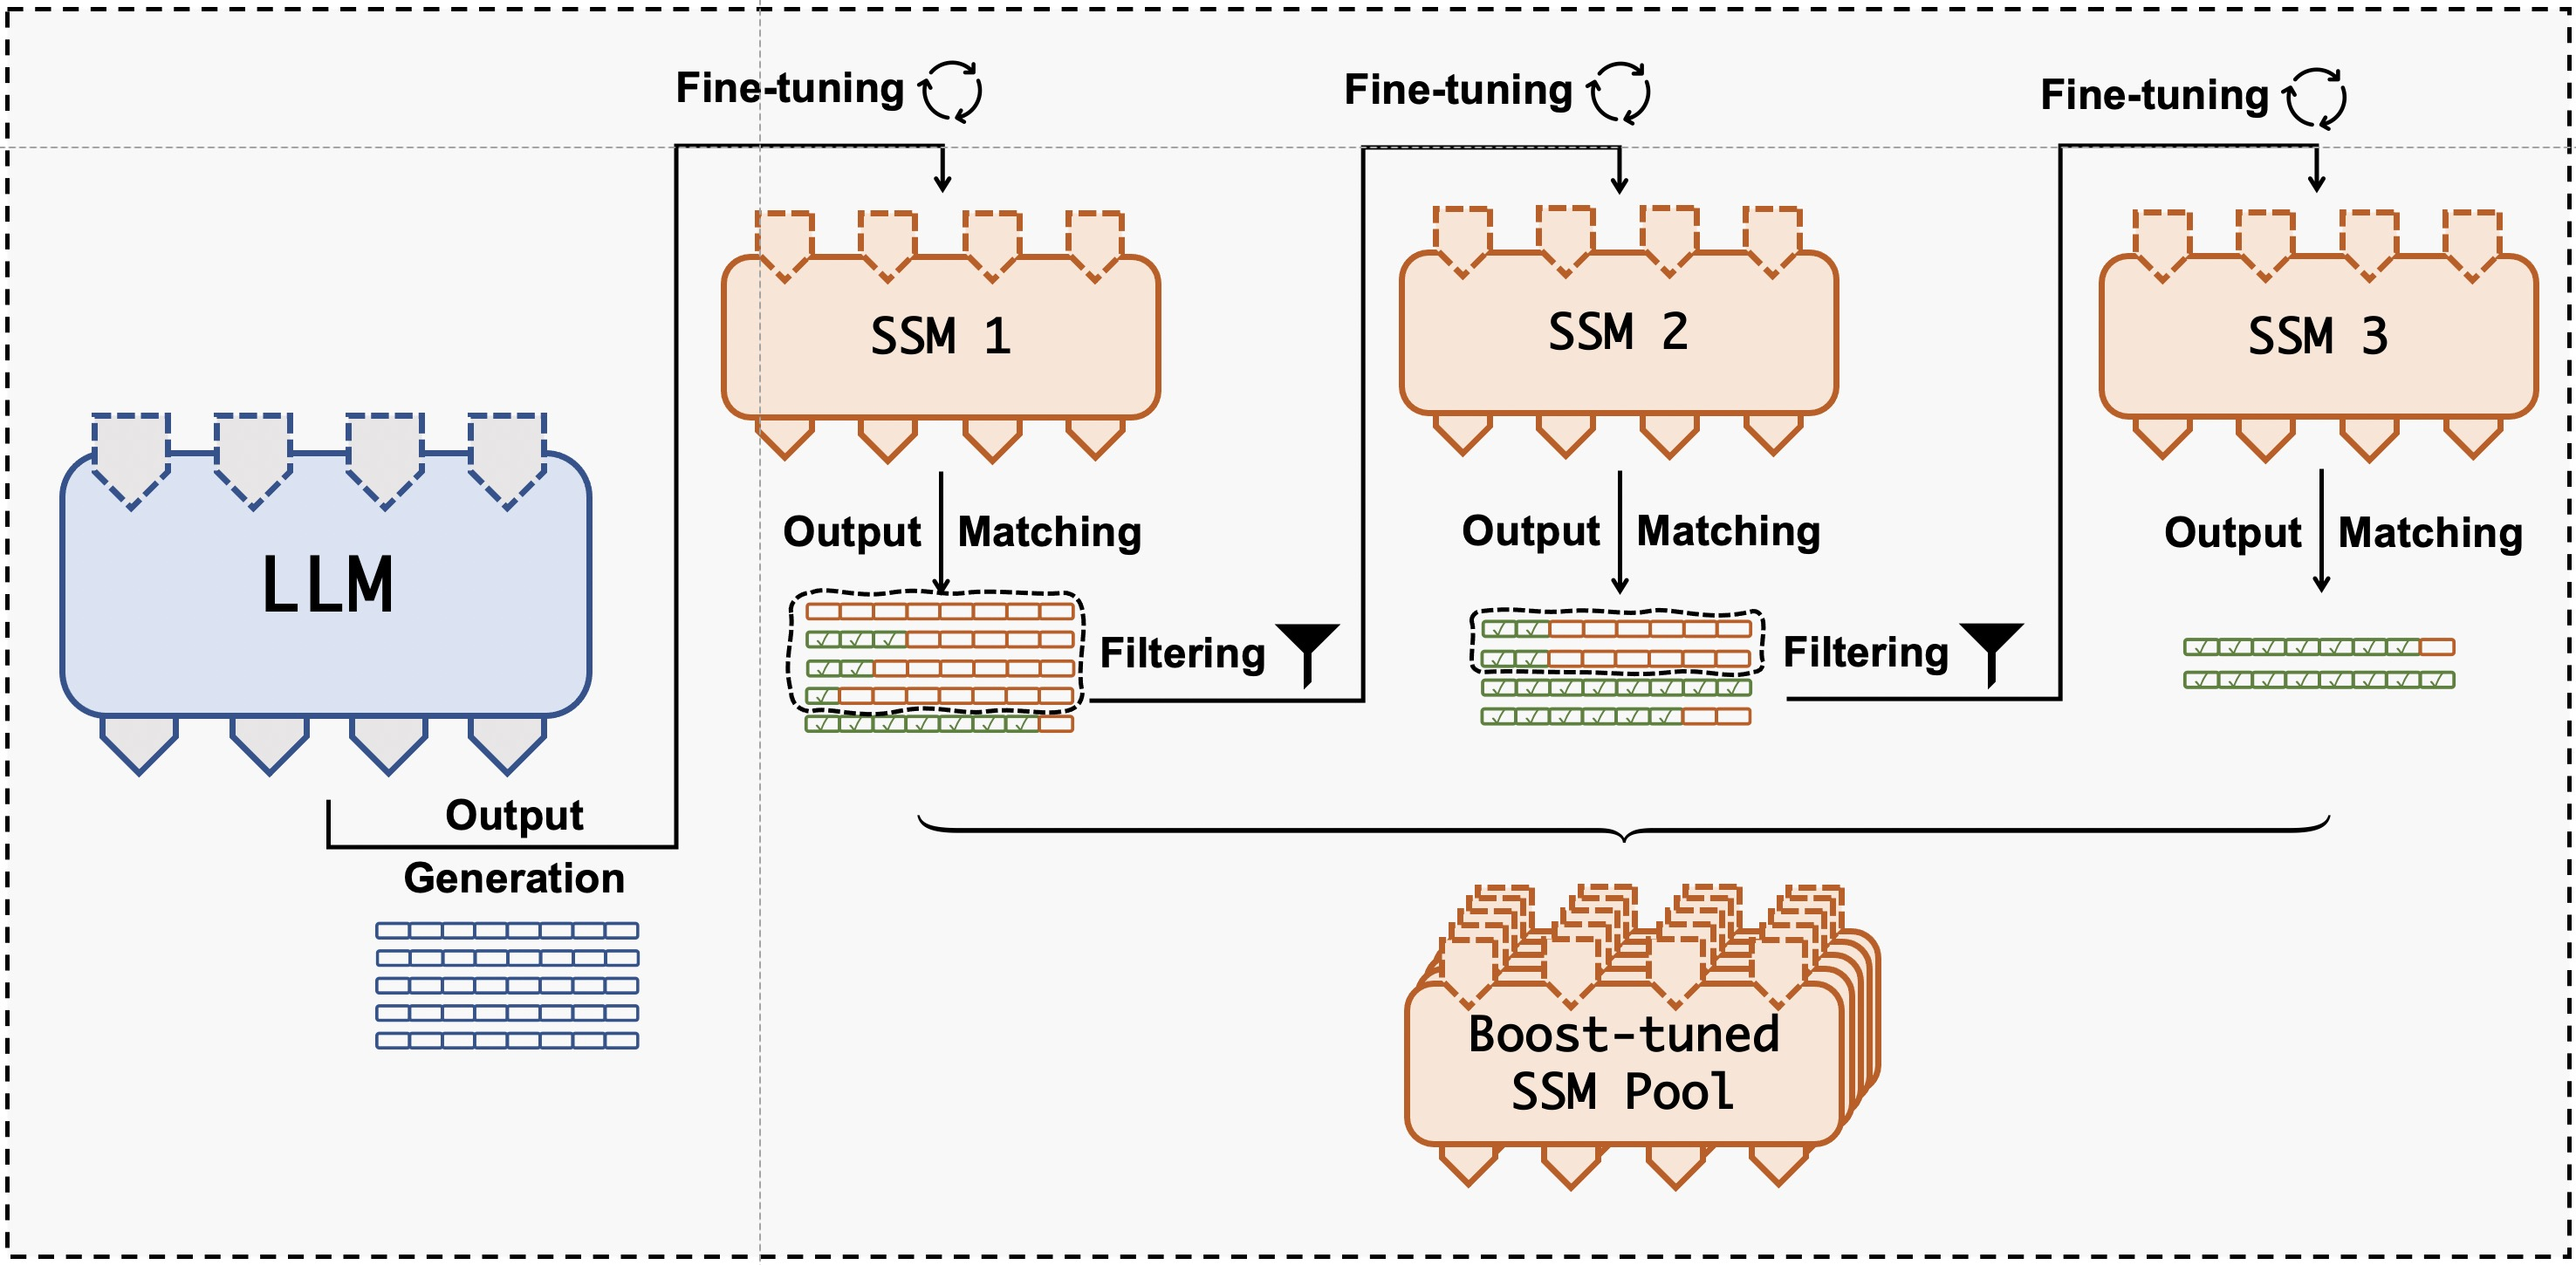
\includegraphics[scale=0.12]{figs/boost_tuning2.jpg}
    %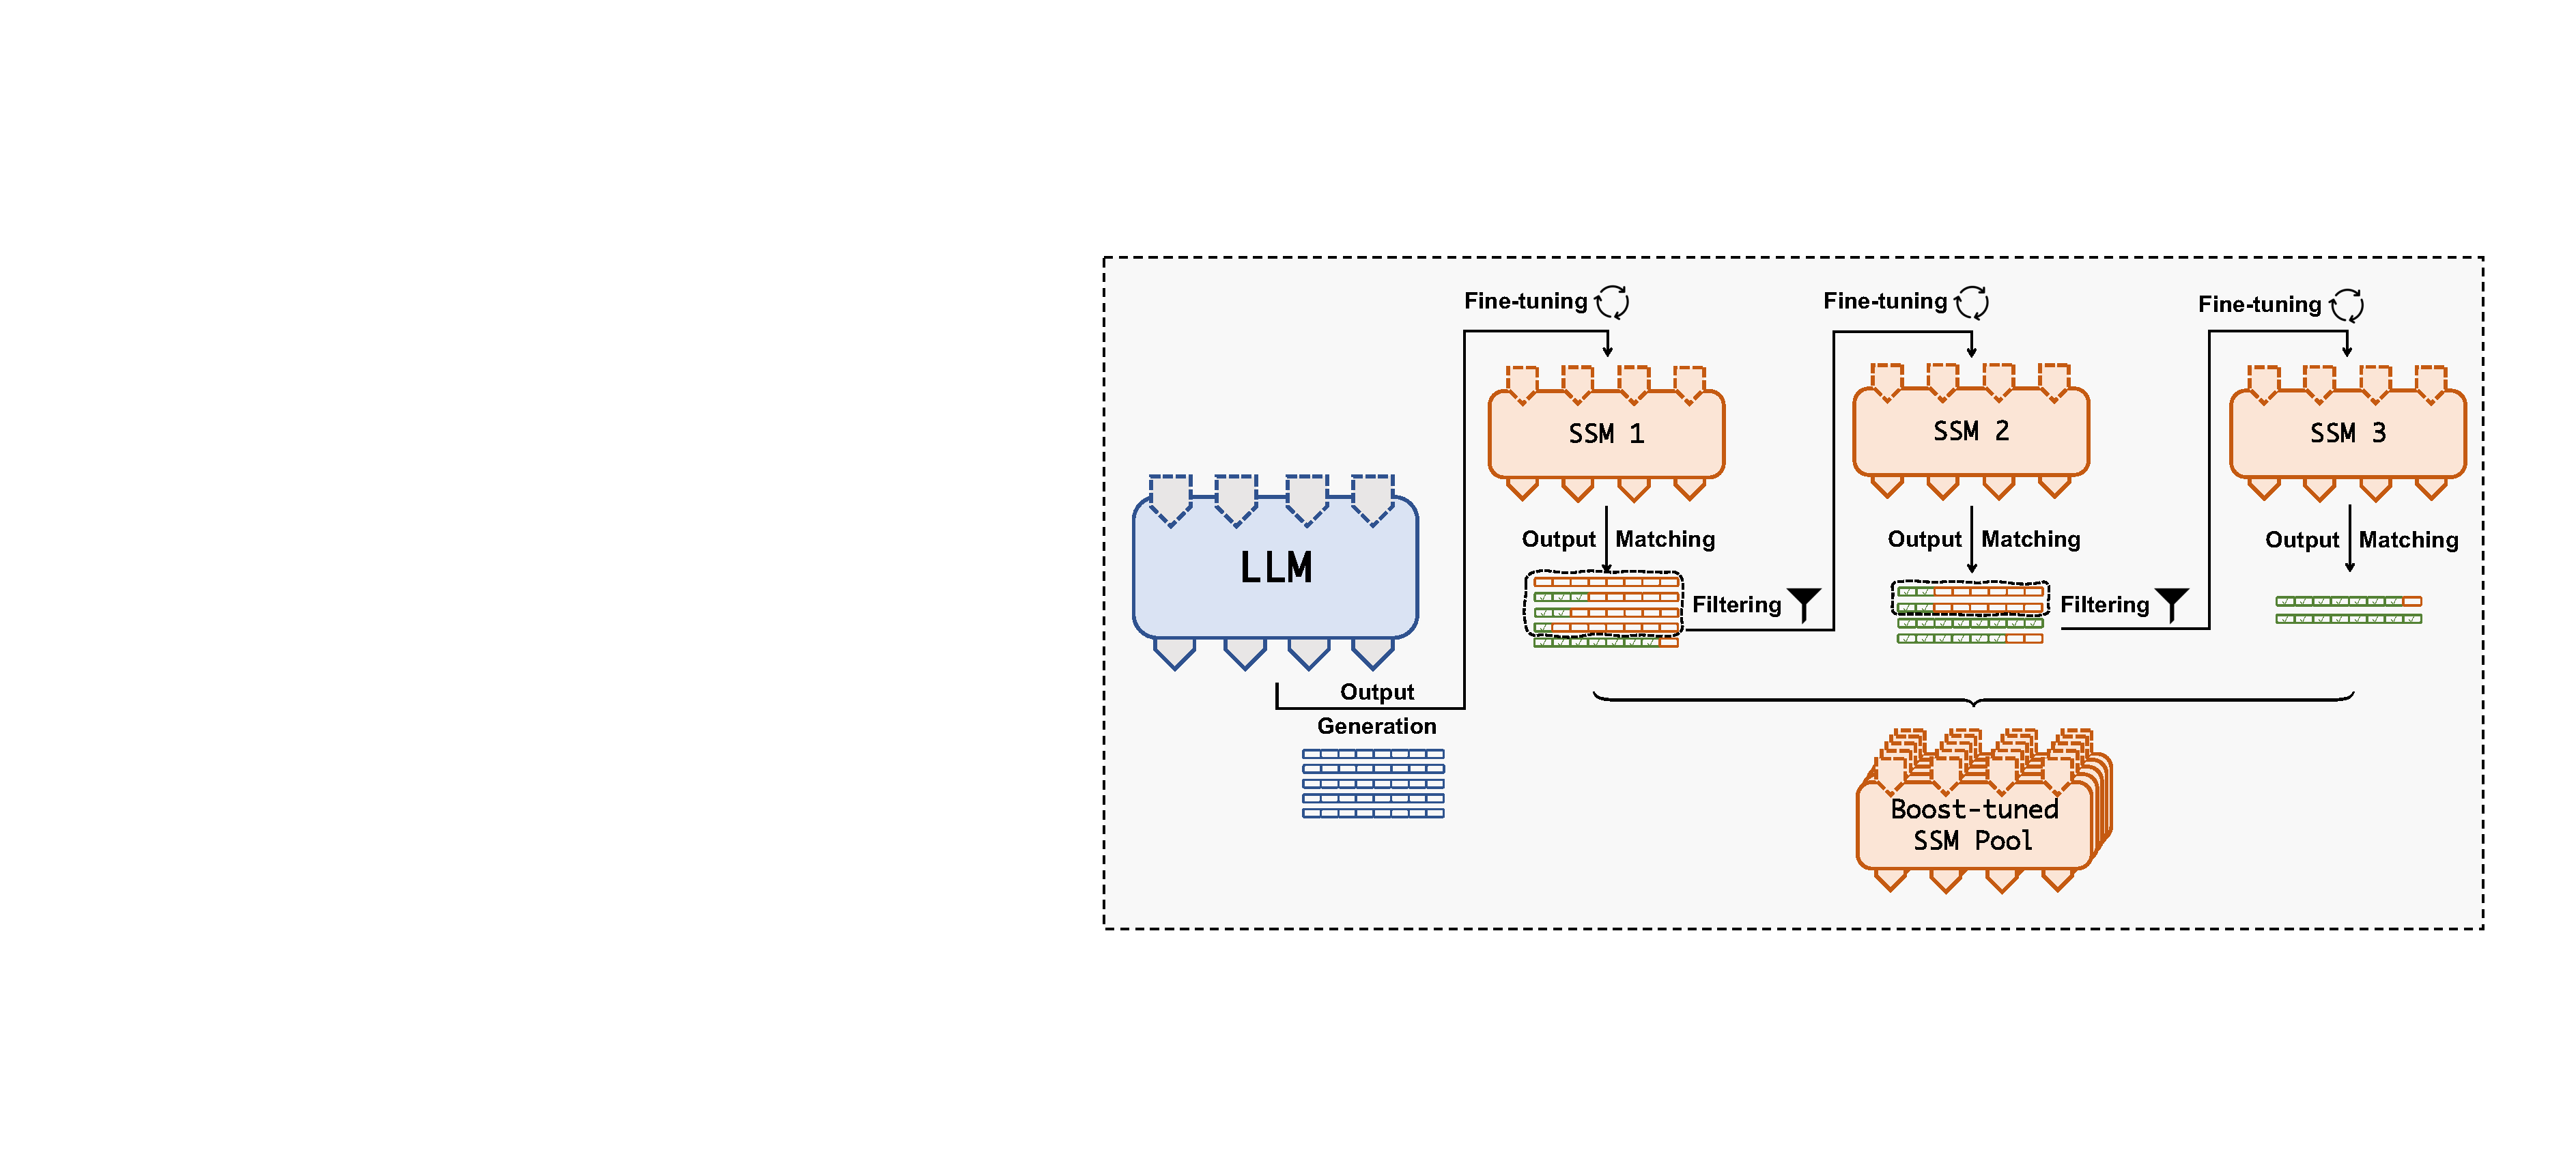
\includegraphics[scale=0.36]{figs/boost_tuning2.pdf}
    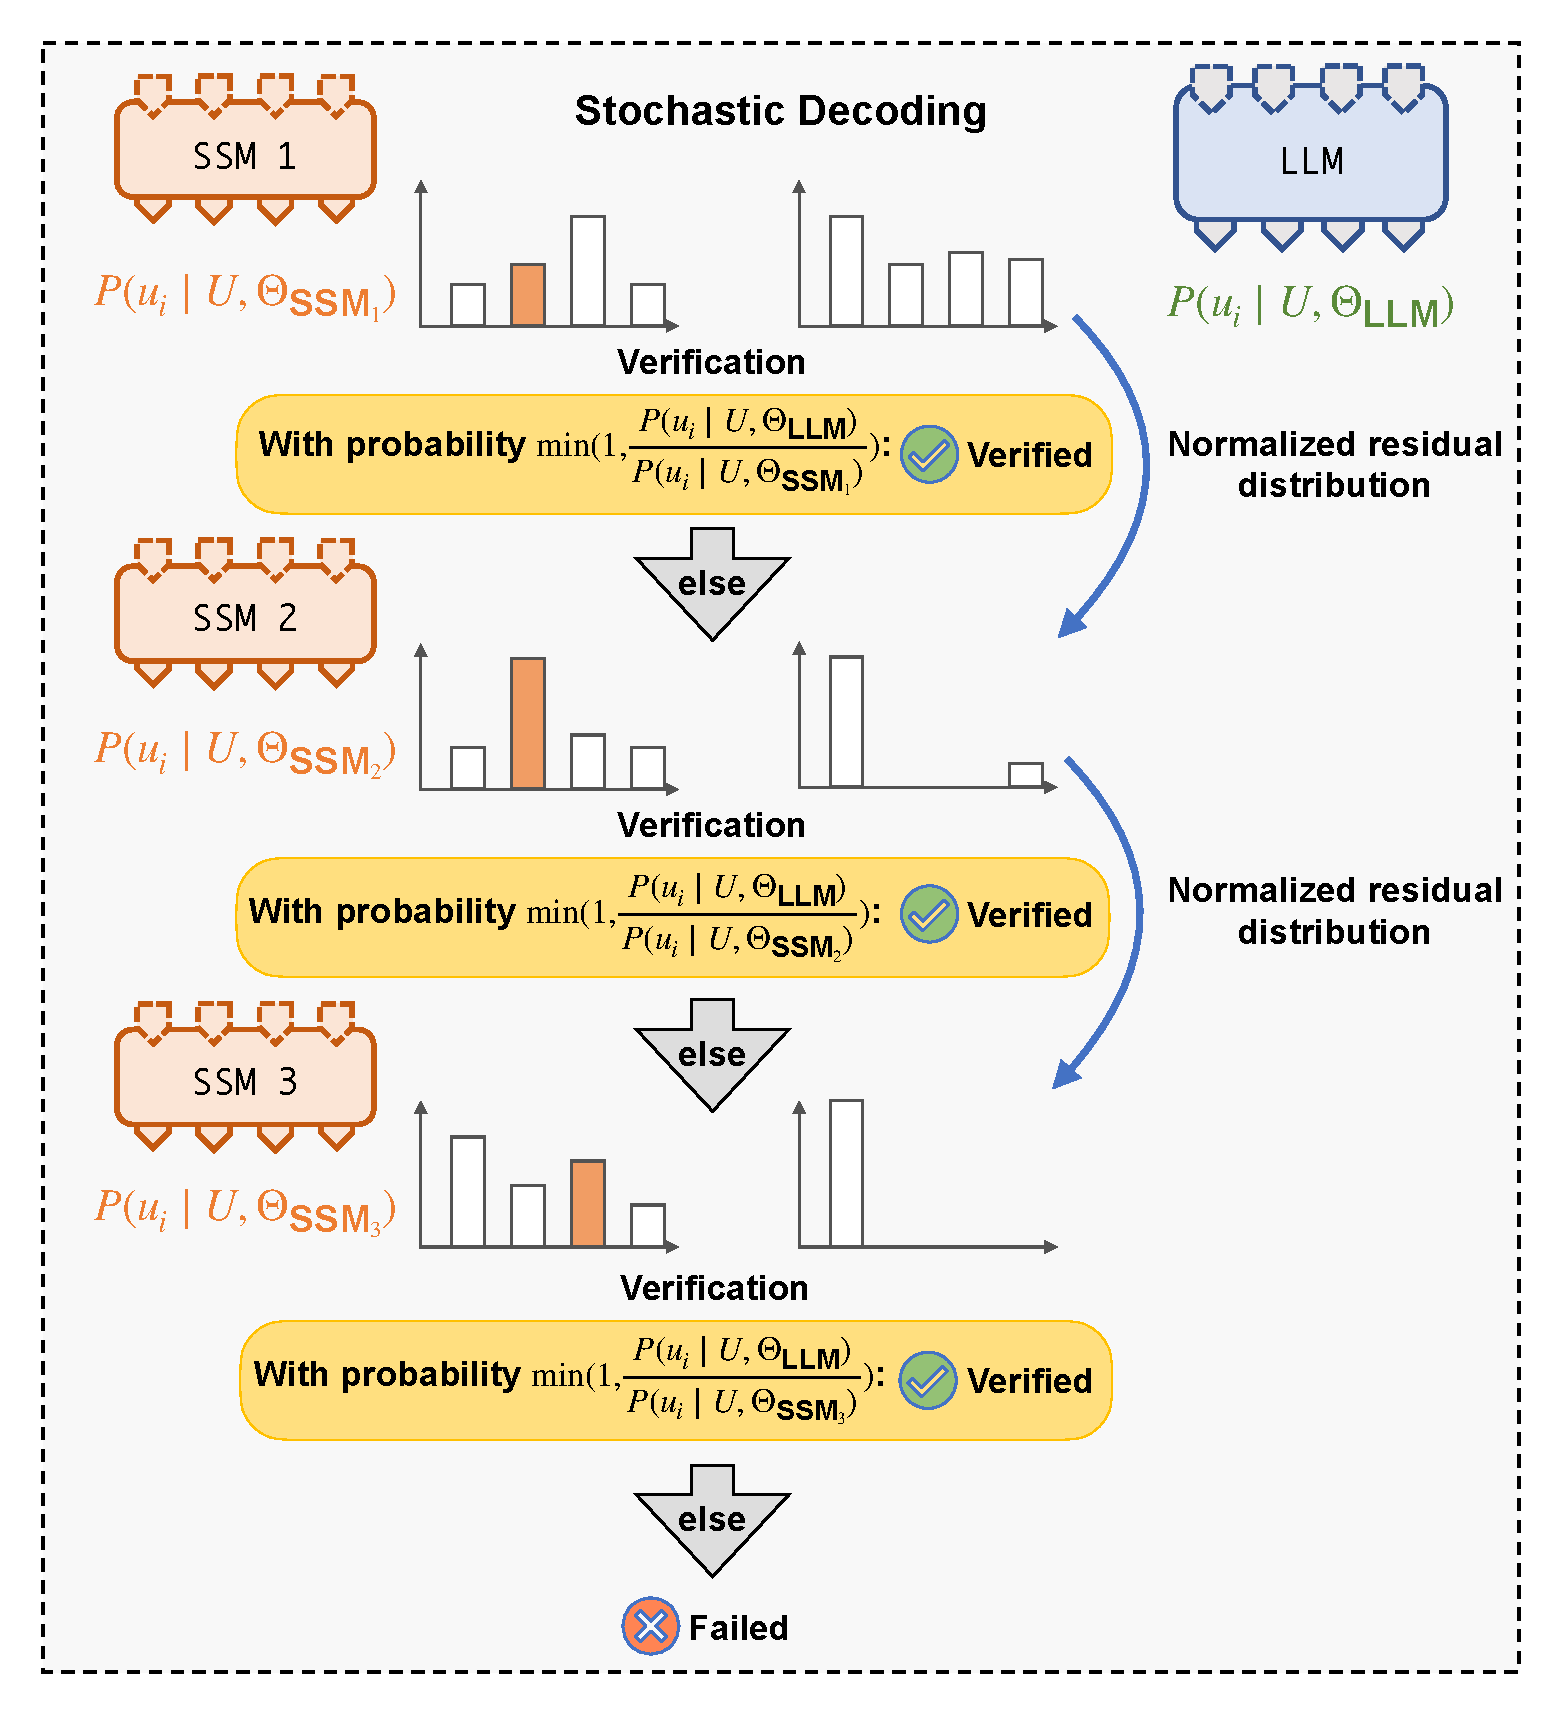
\includegraphics[scale=0.32]{figs/Decodings.pdf}
    \caption{Illustrating the multi-step speculative sampling mechanism for verifying LLMs with stochastic sampling.}
    \label{fig:decodings}
\end{figure}

\paragraph{Greedy decoding.}
Many LLM applications generate tokens using {\em greedy decoding}, which greedily selects the token with the highest likelihood in each decoding step.
The $\textproc{VerifyGreedy}$ function in \Cref{alg2} shows how \Sys verifies a speculated token tree $\m{N}$ with greedy decoding.
\Sys starts from the root of $\m{N}$ and iteratively examines a node's speculated results against the LLM's original output.
%%%
For a node $u\in\m{N}$, \Sys successfully speculates its next token if $u$ includes a child node $v$ (i.e., $p_v = u$) whose token matches the LLM's output (i.e., $t_v = \m{O}(u)$).
In this case, \Sys finishes its verification for node $u$ and moves on to examine its child $v$.
%%%
When the node $u$ does not include a child that contains the LLM's output, \Sys adds $\m{O}(u)$ as a verified node in $\m{N}$ and terminates the verification process.
%%%
Finally, all verified nodes are appended to the current generated token sequence $\m{V}$.
%%%
Token tree verification allows \Sys to opportunistically decode multiple tokens (instead of a single token in the incremental decoding approach), while preserving the same generative performance as incremental decoding.

% \begin{algorithm}
% %\small
% \caption{Generalized speculative sampling (GSS). We use $p(\cdot)$ and $q(\cdot)$ to denote the LLM's token sampling probability and SSMs' token sampling probability respectively.}
% \label{alg:gss}
% \begin{algorithmic}[1]
% \State {\bf Input:} A sequence of input tokens $\m{I}$; LLM sampling temperature $T_{L}$; SSMs sampling temperature $T_{S}$
% \State {\bf Output:} A sequence of generated tokens
% \State $\m{S} = \m{I}$
% \While{true}
% \State $\m{N}, q(\cdot \mid \m{N}/\textrm{Leaf}(\m{N})) = \Call{Speculate}{\m{S}, T_{S}}$
% \State $p(\cdot \mid \m{N}) = \Call{TreeParallelDecode}{\textrm{LLM}, \m{N}, T_{L}}$ 
% %\XM{Hhttps://www.overleaf.com/project/6400b5737cf6fcf36796d963ow about using a function that takes LLM as input to highlight the differences of using LLMs? E.g., t$\gets$Decode(LLM, S) for Algorithm 1 and $\m{O}\gets$ParallelDecode(LLM, $\m{N}$) in Algorithm 2}
% \State $\m{V} = \Call{Verify}{p, q, \m{N}}$
% \For{$t \in \m{V}$}
% \State $\m{S}$.append($t$)
% \If{$t = \langle \textrm{EOS} \rangle$}
% \State {\bf return} $\m{S}$
% \EndIf
% \EndFor
% \EndWhile
% \State
% \Function{Verify}{$p, q, \m{N}$}
% \State $\m{V} = \emptyset$
% \State $u \leftarrow$ the root of token tree $\m{N}$
% \While{$u$ is a non-leaf node}
% \LineComment{get the children nodes of $u$}
% \State $\m{H} = \textrm{child}(u)$ 
%     \While{{\bf not} is\_empty($\m{H}$)}
%     \LineComment{get $q_{i}(\cdot\mid u)$ with the smallest total variation distance w.r.t $p(\cdot\mid u)$}
%     \State $s = \arg\min_{i \in \m{H}} \textrm{TV}\left(p(\cdot\mid u), q_{i}(\cdot\mid u)\right), r \sim U(0, 1), x_s=\m{H}[s]$ 
%         \If{$r \leq \frac{p(x_s \mid u)}{q(x_s \mid u)}$}
%             \State $\m{V}$.append($x_s$)
%             \State $u = x_s$
%             \State {\bf break}
%         \Else
%             \LineComment{normalize the residual distribution between $q(x \mid u)$ and $p(x \mid u)$}
%             \State $p(x \mid u) \coloneqq \textrm{norm}(\max(0, p(x \mid u)-q(x \mid u)))$
%             \State $\m{H}.\textrm{pop}(s)$
%         \EndIf   
%     \EndWhile
% \If{is\_empty($\m{H}$)}
%     \State {\bf break}
% \EndIf
% \EndWhile
% \State $x \sim p(\cdot \mid u)$
% \State $\m{V}$.append($x$)
% \State {\bf return} $\m{V}$
% \EndFunction
% \end{algorithmic}
% \end{algorithm}

\paragraph{Stochastic decoding.}
To improve the diversity of generated tokens, many LLM applications perform {\em stochastic decoding}, which samples a token from a probability distribution $P(u_i | u_0, ..., u_{i-1}; \Theta_{LLM})$, where $U = u_0,...,u_{i-1}$ are previously generated tokens, $u_i$ is the next token to generate, and $\Theta_{LLM}$ represents a parameterized LLM.

To verify a speculated token tree with stochastic decoding, we introduce a {\em multi-step speculative sampling} (MSS) algorithm to conduct verification, whose pseudocode code is shown in the $\textproc{VerifyStochastic}$ function in \Cref{alg2} and illustrated in \Cref{fig:decodings}.
Our method provably preserves an LLM's generative performance as incremental decoding while optimizing the number of speculated tokens that can be verified.
\Cref{thm:stochastic_sampling} proves its correctness.
% \XM{TODO: do we assume only using merge-based speculator here, rather than expansion-based speculator?}
% \ZJ{It supports both}

\begin{theorem}
\label{thm:stochastic_sampling}
For a given $LLM$ and $m$ SSMs (i.e., $SSM_1$,...,$SSM_m$, let $P(u_i | U; \Theta_{LLM})$ be the probability distribution of sampling a token using stochastic decoding, where $U = u_0,...,u_{i-1}$ are previously generated tokens, $u_i$ is the next token to generate, $\Theta_{LLM}$ represents the parameterized LLM. 

Let $P_{\rm{\Sys}}(u_i | U; \Theta_{LLM}, \{\Theta_{SSM_j}\})$ be the probability distribution of sampling token $u_i$ using \Sys's multi-step speculative sampling (see the $\textproc{VerifyStochastic}$ function in \Cref{alg2}), where $\Theta_{SSM_j}$ is the $j$-th parameterized SSM. Then $ \forall U, u_i, \Theta_{LLM}, \Theta_{SSM_j}$ we have
\begin{eqnarray}
P(u_i \mid U; \Theta_{LLM}) = P_{\rm{\Sys}}(u_i \mid U; \Theta_{LLM}, \{\Theta_{SSM_j}\})
\end{eqnarray}
\end{theorem}

%we design a generalized speculative sampling procedure that guarantees the equivalency of the sampling distribution of LLM while maximizing the number of generated tokens per verification step, as shown in~\Cref{alg:gss}. We further present the equivalency proof below.
%%%
A proof of this theorem is presented in~\cite{miao2023specinfer}.
% \Cref{sec:appendix}.

\if 0
Additionally, our generalized speculative sampling procedure has a lower overall rejection probability than a naive method which simply samples from the sampling distribution of the LLM and searches for an SSM sample matching the LLM sample. The proof is presented below.
\fi

We acknowledge that a more straightforward approach to preserving the probability distribution of stochastic decoding is directly sampling the next token $x \sim P(u_i \mid U; \Theta_{LLM})$ and examining whether $x$ is a child node of $u_{i-1}$ in the speculated token tree. We call this approach {\em naive sampling} (NS) and show that \Sys's multi-step speculative sampling has a uniformly lower rejection probability than naive sampling.

\begin{theorem}
\label{theorem:MSS}
    Let $P\left(\textrm{reject} \mid \textrm{MSS}, U, \Theta_{\textrm{LLM}}, \{\Theta_{\textrm{SSM}_j}\} \right)$ denote the probability of rejecting speculation following multi-step speculative sampling with abbreviation $P(\textrm{reject}\mid \textrm{MSS})$, and $P\left(\textrm{reject} \mid \textrm{NS}, U, \Theta_{\textrm{LLM}}, \{\Theta_{\textrm{SSM}_j}\}\right)$ the probability of rejecting speculation following Naive Sampling (NS) with abbreviation $P(\textrm{reject}\mid\textrm{NS})$. Then $\forall U, \Theta_{\textrm{LLM}}, \{\Theta_{\textrm{SSM}_j}\}$, we have $$P(\textrm{reject}\mid \textrm{MSS}) \leq P(\textrm{reject}\mid\textrm{NS})$$
\end{theorem}

We present a proof of~\Cref{theorem:MSS} in~\cite{miao2023specinfer}.
%\Cref{sec:appendix}.

\if 0
\rev{Note that prior sequence-based speculative inference work has introduced the verification algorithm for a single speculative model~\cite{leviathan2022fast, chen2023accelerating} when performing stochastic sampling. Different from these approaches, \Sys leverages multiple boosted SSMs and token trees for improving speculative performance, which requires a verification algorithm that can be generalized to more than one SSM while maximizing the verification success rate. More specifically,~\cite{leviathan2022fast, chen2023accelerating} only verifies against one speculative sampling distribution per step and fails once there is a mismatch, which is not optimal when we have multiple speculative sampling distributions to verify with. As a result, \Sys presents a multi-step verification algorithm (see \textproc{VerifyStochastic} in \Cref{alg2}) that can verify against all branches of a token to maximize the success rate while preserving equivalence as incremental decoding. [5, 26]'s stochastic verification algorithms are thus a special case of \Sys's \textproc{VerifyStochastic} algorithm when there is only a single sequence of speculated tokens.  
}
\fi

\rev{Note that prior work has introduced single-step speculative sampling for sequence-based speculative inference~\cite{leviathan2022fast, chen2023accelerating}. Different from these approaches, \Sys leverages token trees for improving speculative performance, which requires a different verification algorithm. As a result, \Sys performs multi-step verification (see \textproc{VerifyStochastic} in \Cref{alg2}) across all branches of a token to maximize the success rate while preserving equivalence as incremental decoding.
The proposed MSS algorithm not only works for  merge-based method with multiple SSMs, but also supports expansion-based method with one SSM and top-$k$ sampling.
}

\section{System Design and Implementation}

\begin{figure}
    \centering
    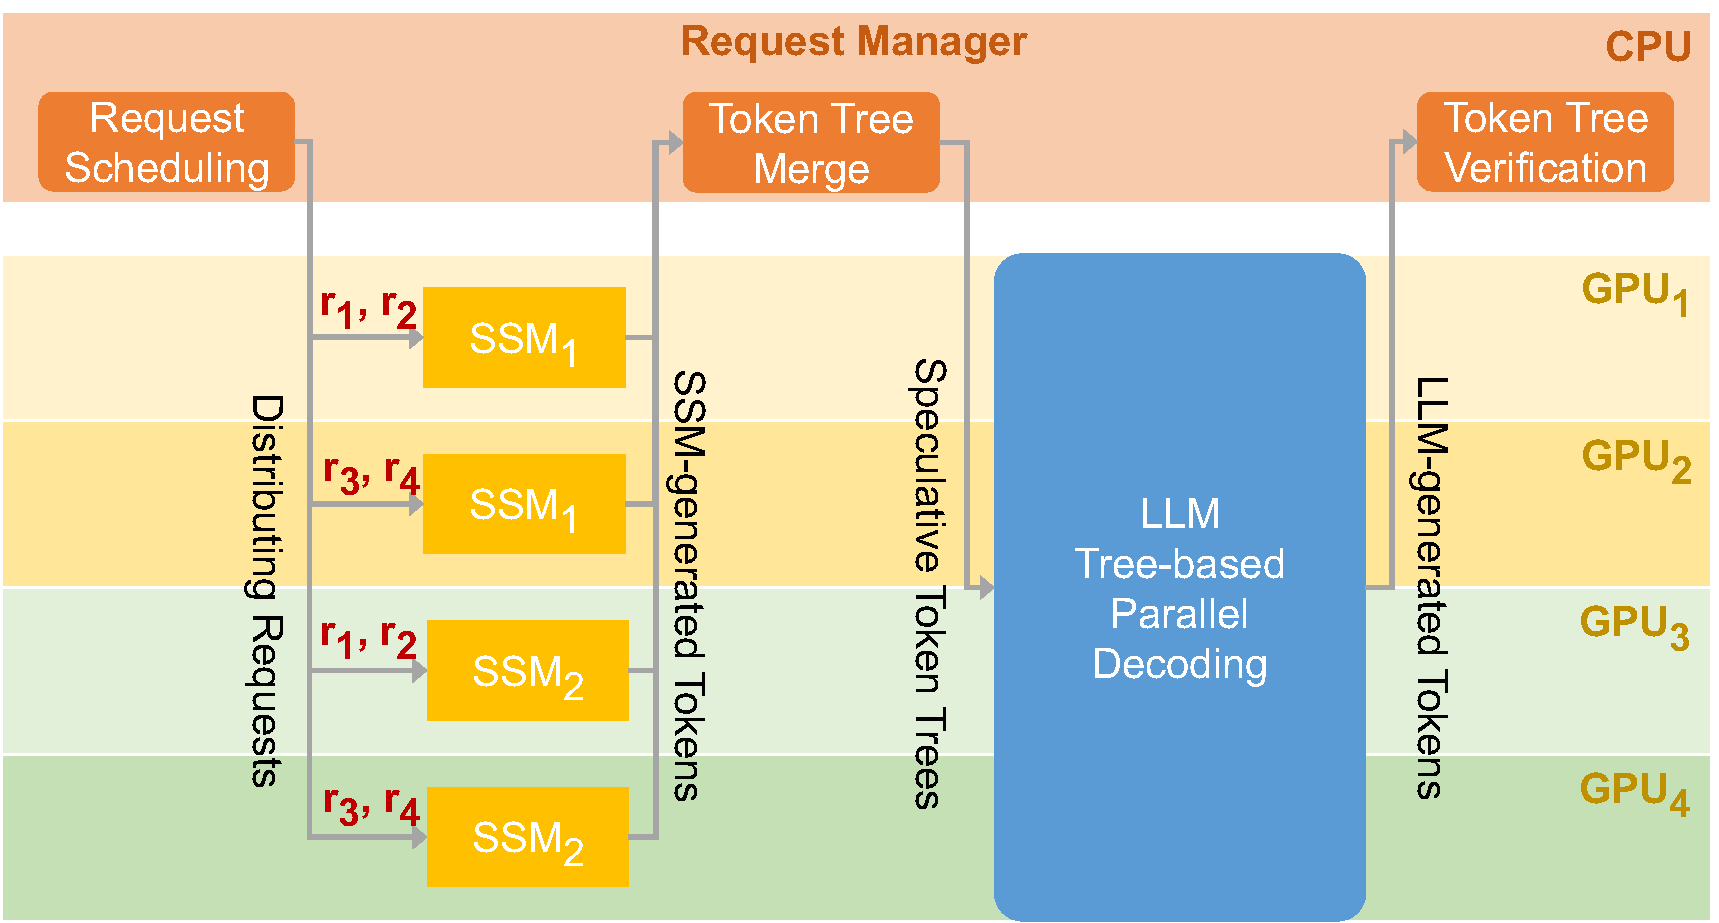
\includegraphics[scale=0.28]{figs/workflow.pdf}
    \caption{\Sys's workflow for one iteration of speculative inference and verification. \Sys uses data parallelism to serve SSMs, and combine tensor model parallelism and pipeline model parallelism for serving an LLM.}
    \label{fig:workflow}
\end{figure}

This section describes the design and implementation of \Sys's distributed runtime system (\S\ref{subsec:design} and \S\ref{subsec:implementation}), analyzes the computation and memory overheads of speculation and verification (\S\ref{subsec:overhead}), and introduces potential LLM applications that can benefit from \Sys's techniques (\S\ref{subsec:application}).

\subsection{\Sys's Runtime Design}
\label{subsec:design}
\Cref{fig:workflow} shows the workflow for one iteration of speculative inference and verification.
%%%
\Sys's {\em request manager} receives LLM serving requests and schedules these requests for serving by adapting the {\em iteration-level scheduling} policy from Orca~\cite{yu2022orca}. Specifically, \Sys iteratively selects requests from a pool of pending requests and performs one iteration of speculative inference and token tree verification for the selected requests. Since SSMs are small and can fit in one GPU, \Sys equally distributes GPUs across SSMs and serves these SSMs using data parallelism. 
For example, \Cref{fig:workflow} shows how \Sys serves two SSMs and four requests (i.e., $r_1$, $r_2$, $r_3$, and $r_4$) on four GPUs.
%%%
The SSM-generated tokens are sent back to the request manager, which produces a speculated token tree for each request using the tree merge algorithm introduced in \S\ref{sec:verification}.

\Sys serves an LLM using the hybrid parallelization strategy introduced in Megatron-LM~\cite{shoeybi2020megatronlm}, which uses tensor model parallelism for parallelizing each Transformer layer across GPUs within a node, and uses pipeline model parallelism for partitioning Transformer layers across nodes. 
All GPUs perform the tree-based parallel decoding (see \S\ref{subsec:optimization}) to compute tree attention scores and send the LLM-generated tokens back to the request manager, which finally verifies the speculated tokens against the LLM's output (see \S\ref{subsec:verification}). 

Note that the overhead introduced by the request manager (i.e., request scheduling, token tree merge, and verification) is negligible compared to the execution time of LLM inference. In addition, \sys's request manager and GPU workers only communicate tokens and do not transfer the vector representations of these tokens, which again introduces negligible communication overheads.

%\vspace{-4mm}

\paragraph{Continuous batching.}
\Sys uses {\em continuous batching} introduced in Orca~\cite{yu2022orca} to serve multiple LLM inference requests in parallel. Specifically, \sys schedules LLM execution at the granularity of iterations instead of requests. After each LLM decoding iteration, \sys checks each request's status and sends the generated results of all finished requests to the client. This design also allows \sys to start processing newly arrived requests without waiting for all current requests to complete.

\subsection{\Sys's Implementation}
\label{subsec:implementation}
\Sys was implemented on top of FlexFlow~\cite{jia2019flexflow, unger2022unity}, a distributed multi-GPU runtime for DNN computation. FlexFlow exposes an API that allows users to define a DNN model in terms of its layers.
\rev{It is compatible with PyTorch’s model definition due to the alignment of underlying operators. For example, the open-source LLMs from HuggingFace~\cite{huggingface} can be directly imported into \sys for serving without modification.}
Users can also provide a parallelization strategy, specifying the degree of data, model, and pipeline parallelism for each layer. 
%During the training phase, FlexFlow can automatically discover the best parallelization plan, which can then be saved and reused in the inference stage. 
%
A DNN is represented as a computational graph where each node is a region of memory, and each edge is an operation on one or more regions. Operations can be represented using three levels of abstraction: layers, operators, and tasks. The FlexFlow compiler transforms the computational graph from the highest abstractions (i.e., layers) to the lowest (i.e., tasks). Tasks are also the unit of parallelization; they are non-preemptible, and are executed asynchronously. 

\rev{
\paragraph{CUDA kernel optimizations.}
Directly launching cuBLAS and cuDNN kernels for calculating attention results in high kernel launch overhead and does not leverage the shared memory available on modern GPUs. To address this inefficiency, \Sys uses a customized kernel built on top of FasterTransformer~\cite{fastertransformer} for computing attention.
Within this kernel, each thread block computes a single head for a single request. The process begins with loading the query tensor into GPU shared memory accessible by all threads within a thread block. Each thread then performs a segment of the query/key product and broadcasts the result to other threads for computing the max query/key product and exponential sum.
To support tree-based parallel decoding, \sys computes all tokens within a tree in parallel and leverages the topology-aware causal mask to preserve casuality.}

\if 0
In the standard implementation of the attention mechanism, the computation of Q, K, V (Query, Key, Value) matrices and their subsequent output projection are typically consolidated within a single {\tt cublasGemmEx} function. Therefore, our optimization efforts are primarily directed toward the attention score computation phase. A challenge arises when dealing with multiple heads in the transformer architecture; the requirement to segment each head prevents the amalgamation of computations across different requests into a single operation. Consequently, conventional methods often incorporate an additional loop, where each iteration processes a singular request. This process encompasses two {\tt cublasBatchedGemm} operations and a softmax function. However, this approach introduces substantial kernel launch overhead, particularly noticeable when handling large batch sizes. To address this inefficiency, we developed a custom kernel specifically for the attention score computation, circumventing the constraints inherent to the cuBLAS API and consequently enhancing overall performance. This kernel is modified from FasterTransformer~\cite{fastertransformer}. Within our custom kernel, each thread block is assigned the task of computing a single head for a specific request. The process begins with loading the Query into shared memory, accessible by all threads within the block.  Then the kernel allocates multiple threads to each key based on predefined configurations and performs a segment of the QK product. Subsequently, these partial values are broadcast to other threads for the computation of the max QK product and the exponential sum, which are used in the softmax calculation. In addition, our custom kernel supports the Tree-based Parallel Decoding mentioned in Section 4.2. For decoding sequences in tree structures, we load all keys and values at once. This allows for the calculation of the product between all query tokens (nodes) and each key/value. If a key/value token is positioned before the root node of the tree, we retain the QK product. When the key/value is part of the tree, we consult the topology-aware causal mask to determine its relevance to the query token. If they are not relevant, the QK product is set to zero. This customization in our kernel significantly reduces launch overhead and maximizes GPU resource utilization.
\fi

\subsection{Overhead of Speculation and Verification}
\label{subsec:overhead}
\Sys accelerates generative LLM inference at the cost of additional memory and computation overheads. This section analyzes these overheads and shows that they are generally one or two orders of magnitude smaller than the memory and computation cost of executing LLM inference.

\paragraph{Memory overhead.} The memory overhead of \Sys's speculation-verification approach comes from two aspects. First, in addition to serving an LLM, \Sys also needs to allocate memory for saving the parameters of one or multiple SSMs, which collectively speculate the LLM's output. 
Our evaluation shows that \Sys can achieve significant performance improvement by using SSMs 100-1000$\times$ smaller than the LLM. As a result, hosting each SSM increases the overall memory requirement by less than 1\%. 
A second source of memory overhead comes from the token tree verification engine, which verifies an entire token tree instead of decoding a single token. 
%%%
Therefore, additional memory is needed for caching the keys and values, and storing the attention scores for all tokens. 
%%%
Due to the necessity for supporting very long sequence length in today's LLM serving, we observe that the memory overhead associated with token tree is negligible compared to key-value cache.
%%%
%For example, GPT-4 supports processing up to 32K tokens in a single request; our evaluation shows that a token tree of size 40 already allows \Sys to match 3.7 tokens on average.

\paragraph{Computation overhead.} Similarly, the computation overhead introduced by speculation and verification also comes from two aspects.
%%%
First, \Sys needs to run SSMs in the incremental-decoding mode to generate candidate tokens. When multiple SSMs are employed, \sys processes these SSMs in parallel across GPUs to minimize speculation latency.
%\Sys processes the SSMs in parallel across GPUs to minimize the latency for generating a speculated token tree.  \XM{TODO: update}
%Our evaluation shows that the latency of running a SSM in the incremental-decoding mode is 3.7$\times$ better than that of an LLM.
%%%
Second, \Sys verifies a token tree by computing the attention outputs for an entire token tree, most of which do not match the LLM's output and therefore are unnecessary in the incremental-decoding inference.
%%%
However, the key-value cache mechanism of existing LLM inference systems prevents them from serving a large number of requests in parallel, resulting in under-utilized computation resources on GPUs when serving LLMs in incremental decoding. \Sys's token tree verification leverages these under-utilized resources and therefore introduces negligible runtime overhead compared to incremental decoding.

\subsection{Applications}
\label{subsec:application}
Our speculative inference and token tree verification techniques can be directly applied to a variety of LLM applications. We identify two practical scenarios where LLM inference can significantly benefit from our techniques.

\paragraph{Distributed LLM inference.} 
The memory requirements of modern LLMs exceed the capacity of a single compute node with one or multiple GPUs, and the current approach to addressing the high memory requirement is distributing the LLM's parameters across multiple GPUs~\cite{miao2023spotserve}.
For example, serving a single inference pipeline for GPT-3 with 175 billion parameters requires more than 16 NVIDIA A100-40GB GPUs to store the model parameters in single-precision floating points.
%%%
Distributed LLM inference is largely limited by the latency to transfer intermediate activations between GPUs for each LLM decoding step. 
%%%
While \Sys's approach does not directly reduce the amount of inter-GPU communications, its verification mechanism can increase the communication granularity and reduce the number of decoding steps.


\paragraph{Offloading-based LLM inference.}
Another practical scenario that can benefit from \Sys's techniques is offloading-based LLM inference, which leverages 
CPU DRAM to store an LLM's parameters and loads a subset of these parameters to GPUs for computation in a pipeline fashion~\cite{sheng2023highthroughput}.
%%%
By opportunistically verifying multiple tokens, \Sys can reduce the number of LLM decoding steps and the overall communication between CPU DRAM and GPU HBM.
%\section{Discussion}

\section{Evaluation}
\label{sec:eval}

\begin{figure*}
    \centering
    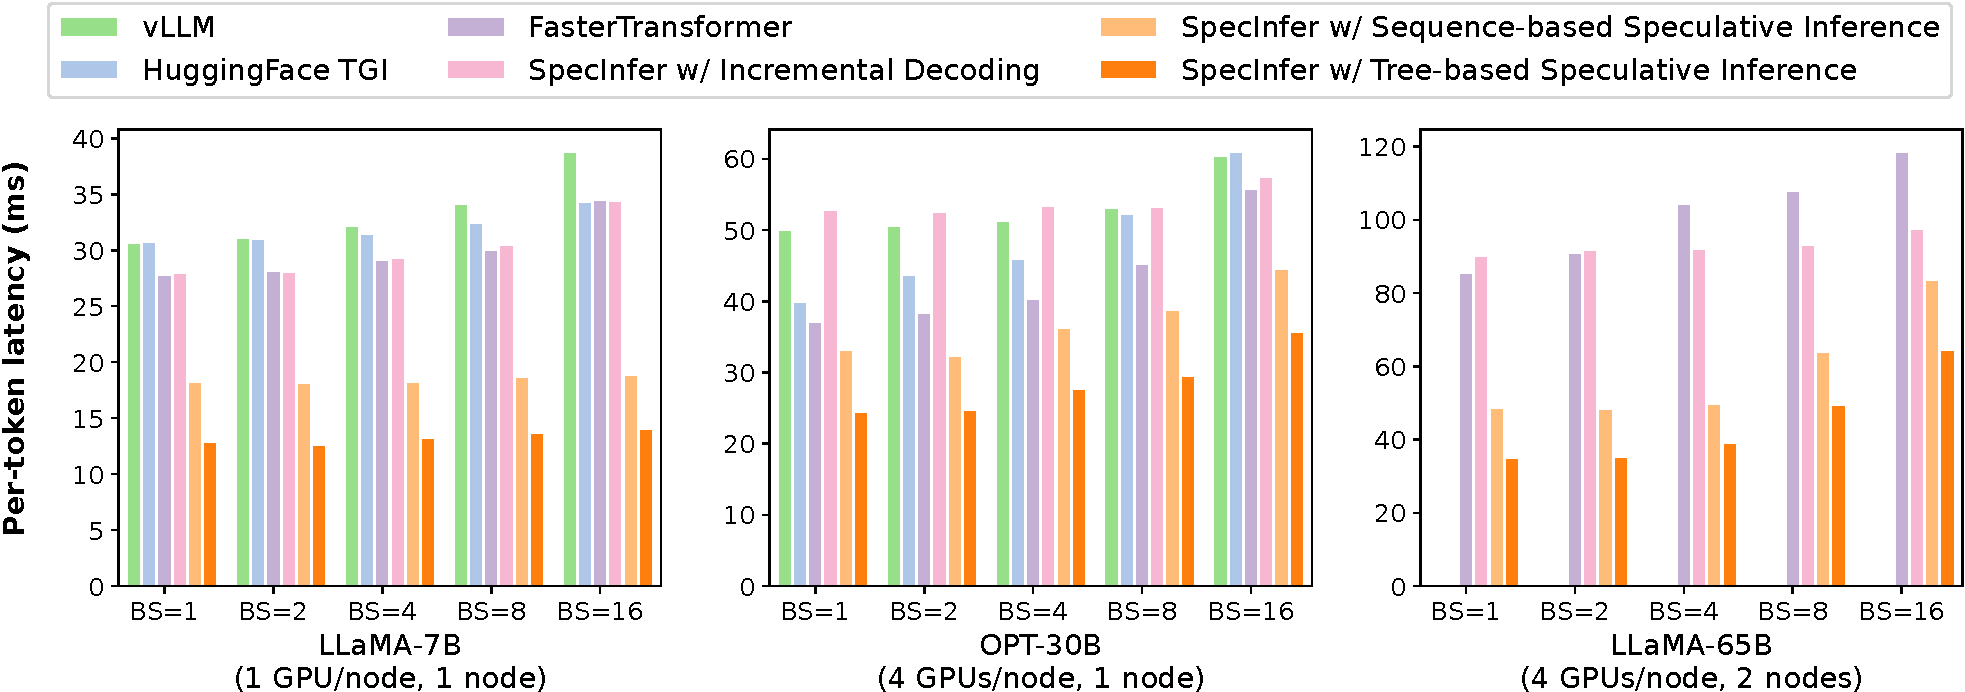
\includegraphics[scale=0.52]{figs/revised_end_to_end2-crop.pdf}
    \caption{\rev{Comparing the end-to-end inference latency of \Sys with existing systems. Numbers in parenthesis show the number of GPUs and compute node used to serve each LLM. All systems parallelize LLM inference by combining tensor model parallelism (within a node) and pipeline parallelism (across nodes).}
    %We use \llama-7B as the LLM and all SSMs are derived from \llama-68M.
    %The performance is normalized by incremental decoding, and the numbers on the \Sys bars indicate the speedups over incremental decoding.
    }
    \label{fig:latency}
\end{figure*}

\subsection{Experimental Setup}
\label{subsec:setup}

\paragraph{LLMs.} To compare the runtime performance of \Sys with existing LLM serving systems, we evaluate these systems using two publicly available LLM families: OPT~\cite{zhang2022opt} and \llama~\cite{touvron2023llama}. 
%%%
More specifically, we select \llama-7B, OPT-13B, OPT-30B, and \llama-65B as the LLMs, and \llama-68M and OPT-125M as the SSMs.
%%%
%\Cref{sec:cbt_method} describes how \Sys collectively boost-tunes multiple SSMs from the pre-trained one.
The pre-trained model parameters for the LLMs and SSMs were obtained from their HuggingFace repositories~\cite{huggingface}, and we describe how \Sys collectively boost-tunes multiple SSMs in~\cite{miao2023specinfer}.
% \Cref{sec:cbt_method}.
%%%
%\Cref{subsec:eval_boost_tuning} evaluates how collective boost-tuning can further improve speculation performance.

\paragraph{Datasets.} We evaluate \Sys on five datasets: Chatbot Instruction Prompts (CIP)~\cite{chatbot2023}, ChatGPT Prompts (CP)~\cite{mohamed2023chatgpt}, WebQA~\cite{berant-etal-2013-semantic}, Alpaca~\cite{alpaca, peng2023instruction}, and PIQA~\cite{Bisk2020}. 
%%%
We only use the prompts/questions from these datasets to form our input prompts to simulate real-world conversation traces.
%%%
%We randomly selected at most 1000 prompts from each dataset in our evaluation.


\paragraph{Platform.} The experiments were conducted on two AWS {\tt g5.12xlarge} instances, each of which is equipped with four NVIDIA A10 24GB GPUs, 48 CPU cores, and 192 GB DRAM. Nodes are connected by 100 Gbps Ethernet.
%\Sys serves OPT-30B and \llama-30B in half-precision floating points across four A10 GPUs using tensor model parallelism.
%OPT-66B and \llama-65B do not fit on four A10 GPUs, therefore \Sys serves these two LLMs on eight A10 GPUs across two compute nodes.
%The LLMs used in our evaluation do not fit on a single T4 GPU. 
%Therefore \Sys performs LLM inference in single-precision floating points and serves the LLMs across the four GPUs using pipeline model parallelism.
%%%
%\Sys serves each SSM on a dedicated GPU and runs these SSMs in parallel for a given sequence of tokens.

Our experiments use the expansion-based method (see \Cref{sec:speculation}) for constructing token trees and use the expansion configuration $\langle 1, 1, 3, 1, 1, 1, 1, 1\rangle$, which provides good results for our benchmarks. We analyze the impact of expansion configurations in \S\ref{subsec:eval_token_tree}, evaluate tree-based parallel decoding and multi-step speculative sampling in \S\ref{subsec:eval_tree_based_decoding} and \S\ref{subsec:eval_msss}, and finally compares the expansion- and merge-based tree construction methods in~\cite{miao2023specinfer}.
% \Cref{sec:eval_tree_construction_methods}.

%\Cref{subsec:eval_token_tree} evaluates the impact of different tree construction methods.
%For all experiments in \Cref{subsec:eval_distributed} and \Cref{subsec:eval_offload}, \Sys uses two SSMs and a speculation depth of 8, which achieves good performance in practice. \XM{\Cref{subsec:eval_boost_tuning}} evaluates how different numbers of SSMs affect \Sys's performance.

\subsection{Distributed LLM Inference}
\label{subsec:eval_distributed}
We compare the end-to-end distributed LLM inference performance among \Sys, vLLM~\cite{vllm}, HuggingFace Text Generation Inference (TGI)~\cite{huggingface_tgi}, and FasterTransformer~\cite{fastertransformer} on \llama-7B, OPT-30B, and \llama-65B.
For \llama-7B and OPT-30B, all systems serve the two LLMs in half-precision floating points across one and four A10 GPUs using tensor model parallelism.
\llama-65B do not fit on four GPUs on a single node, therefore both FasterTransformer and \Sys serve it on eight A10 GPUs on two nodes by combining tensor model parallelism within each node and pipeline model parallelism across nodes.
%%%
vLLM and HuggingFace TGI do not support pipeline model parallelism and cannot serve an LLM on multiple nodes.

To rule out potential effects of our system implementation, we also evaluate \Sys with two additional configurations. First, \sys with {\em incremental decoding} evaluates the runtime performance of our implementation when the speculator generates empty token trees, and the verifier verifies exactly one token in each decoding step.
Second, \sys with {\em sequence-based speculative inference} serves as a reference for existing speculative inference system and is enabled by using a single pre-trained SSM and sequence-based decoding.

We use prompts from the five datasets described in \S\ref{subsec:setup}. For each prompt, we let all systems generate up to 128 new tokens and report the average per-token latency in \Cref{fig:latency}.
%%%
Note that \Sys may generate more than 128 new tokens since the verifier can verify multiple tokens in each iteration. 
In this case, we truncate \Sys's output to 128 tokens.
\Sys with incremental decoding achieves on-par performance as existing  systems. This is because all systems use the same strategies to parallelize LLM inference across GPUs and use the same kernel libraries (i.e., cuDNN, cuBLAS, and cuTLASS) to execute inference computation on GPUs.
%%%
With tree-based speculative inference and verification, \Sys outperforms incremental decoding systems by 1.5-2.5$\times$ for single-node, multi-GPU inference and by 2.4-2.8$\times$ for multi-node, multi-GPU inference, while generating the exact same sequence of tokens as incremental decoding for all prompts.
%%%
\rev{The speedup comes from leveraging spare GPU resources to perform tree-based parallel decoding while maintaining the same per-iteration latency as incremental decoding.}
%The performance improvement is realized by \Sys's ability to verify multiple tokens in a single LLM decoding step.

\rev{Compared to sequence-based speculative inference, \sys's tree-based approach further reduces LLM serving latency by 1.2-1.5$\times$. The improvement is achieved by (1) leveraging token trees to optimize speculative performance, (2) using tree-based parallel decoding to verify an entire token tree in parallel, and (3) performing multi-step speculative sampling to improve verification performance. We further evaluates these aspects in \S\ref{subsec:eval_token_tree}, \S\ref{subsec:eval_tree_based_decoding}, and \S\ref{subsec:eval_msss}.}


\iffinal
Note that \sys's performance improvement over existing systems reduces as the batch size (i.e., number of concurrent requests) increases.
%%%
This is because \sys leverages spare GPU resources to perform tree-based parallel decoding while maintaining the same per-iteration latency as incremental decoding.
%%%
A larger batch size introduces more parallelizable computation for incremental decoding, and thus less spare GPU resources that can be leveraged by \sys.
On the flip side, larger batch sizes also increase the end-to-end latency of each request, as shown in \Cref{fig:latency}.
%%%
Overall, \sys is most beneficial for {\em low-latency} LLM inference.
\fi 

%We compare the end-to-end inference latency between incremental decoding and \Sys on the five prompt datasets. For each prompt dataset, we measured the inference latency of the two approaches on up to 1000 prompts and reported the average inference latency. \Cref{fig:latency} shows the results. Compared to incremental decoding, \Sys reduces the inference latency by 1.9 - 2.7$\times$ while generating the exact same sequence of tokens as incremental decoding for all prompts. The performance improvement is mostly realized by \Sys's ability to verify multiple tokens in a single LLM decoding step.
%%%
%Next, we evaluate how collective boost-tuning and the learning-based speculative scheduler help improve \Sys's inference performance.

\subsection{Offloading-based LLM Inference}
\label{subsec:eval_offload}
\begin{figure}
    \centering
    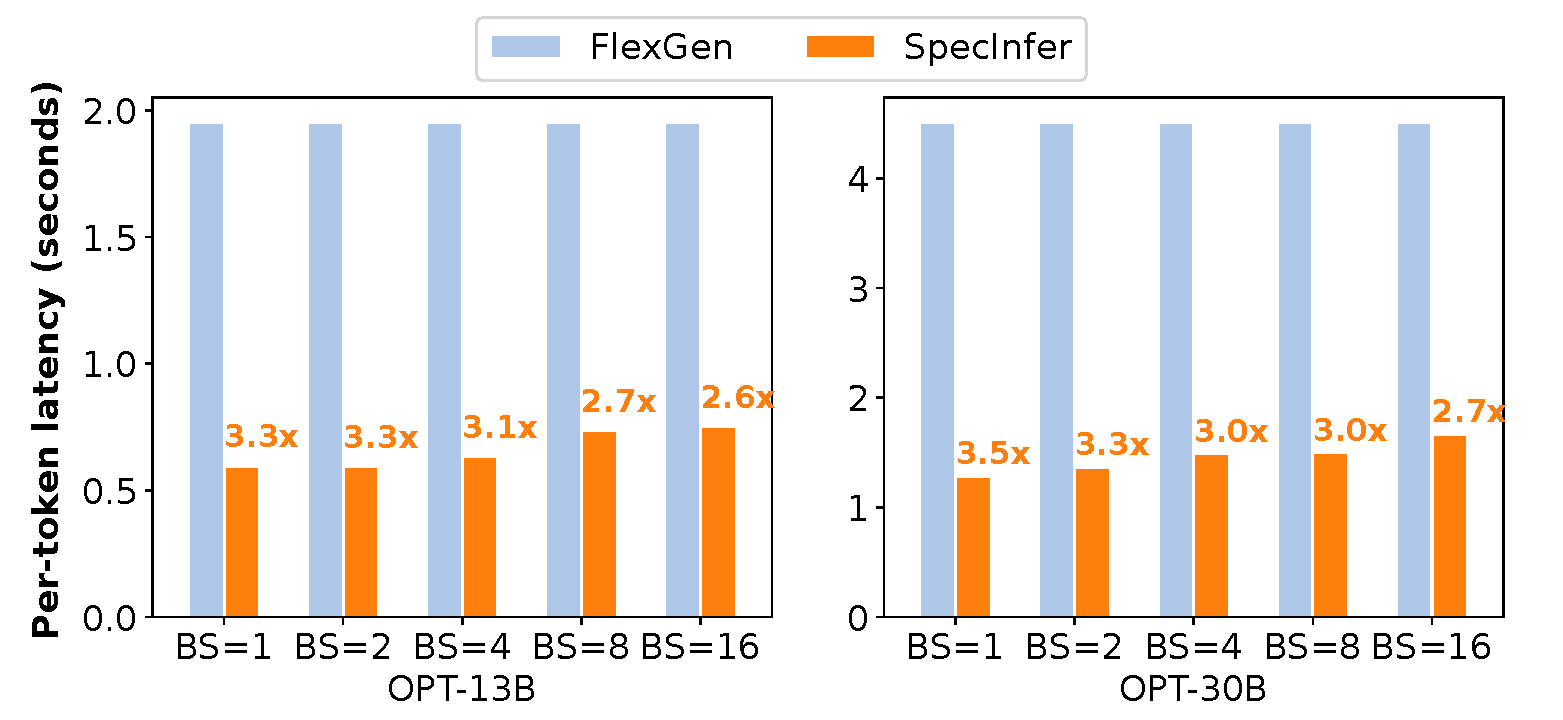
\includegraphics[scale=0.33]{figs/end_to_end_offload2.pdf}
    \caption{Comparing the end-to-end offloading-based inference latency of FlexGen and \Sys. Both FlexGen and \Sys perform model offloading to serve OPT-13B and OPT-30B models on a single 24GB A10 GPU.}
    %\vspace{-4mm}
    \label{fig:eval_offload}
\end{figure}

Another important application of \Sys is offloading-based LLM inference, where the system offloads an LLM's parameters to CPU DRAM and loads a subset of these parameters to GPUs for inference computation in a pipeline fashion.
%%%
We compare the end-to-end offloading-based LLM inference performance between \Sys and FlexGen~\cite{sheng2023flexgen} using a single 24GB A10 GPU and two LLMs (i.e., OPT-13B and OPT-30B), both of which exceed the memory capacity of an A10 GPU and requires offloading for serving. Both \Sys and FlexGen retain all model parameters on CPU DRAM. During computation, the demand weights are loaded from the CPU to the GPU.
%%%
\Cref{fig:eval_offload} shows the results. Compared to FlexGen, \Sys reduces the per-token latency by 2.6-3.5$\times$. 
%%%
Since offloading-based LLM inference is mostly bottlenecked by the communication between CPU DRAM and GPU HBM for loading an LLM's parameters, \Sys's improvement over existing systems is achieved by opportunistically verifying multiple tokens, which in turn reduces the number of LLM decoding steps and data transfers between CPU and GPU.

\subsection{\rev{Token Tree Construction}}
\label{subsec:eval_token_tree}

% \begin{figure}
%     \centering
%     %\subfloat[Greedy sampling CDF.]{
%     %\includegraphics[width=0.33\linewidth]{figs/Greedy sampling CDF.pdf}
%     %}
%     \subfloat[Greedy sampling \textcolor{blue}{This is the CDF figure of greedy decoding}.]{
%     \includegraphics[width=0.5\linewidth]{figs/Greedy decoding CDF.pdf}
%     }
%     \subfloat[Stochastic sampling.]{
%     \includegraphics[width=0.5\linewidth]{figs/Stochastic sampling CDF.pdf}
%     }
%     \caption{CDF figures of greedy sampling, stochastic sampling and greedy decoding. \ZJ{TODO: (1) increase font size for the y-axis title; (2) change the title to ``Average \# verified tokens per decoding step''; (3) add a ``='' between tree width and value}
%     }
%     \label{fig:ssms_greedy_coding}
% \end{figure}



\rev{This section evaluates the expansion-based token tree construction mechanism. We first study how token tree width affects \Sys's speculative performance. In this experiment, we use \llama-7B and \llama-68M as the LLM and SSM, and use the expansion configuration $\langle 1, 1, k, 1, 1, 1, 1, 1\rangle$ (i.e., expanding at the third token), where $k$ is the token tree width.
\Cref{fig:eval_cdf} shows the cumulative distribution function (CDF) of the average number of verified tokens per decoding step for all prompts in the Alpaca dataset~\cite{alpaca}.
%
Compared to sequence-based speculation (i.e., tree width = 1), leveraging token trees can reduce LLM decoding steps by 1.2-1.5$\times$ for greedy decoding and by 1.3-1.4$\times$ for stochastic decoding.}

\begin{figure}
    \centering
    %\subfloat[Greedy sampling CDF.]{
    %\includegraphics[width=0.33\linewidth]{figs/Greedy sampling CDF.pdf}
    %}
    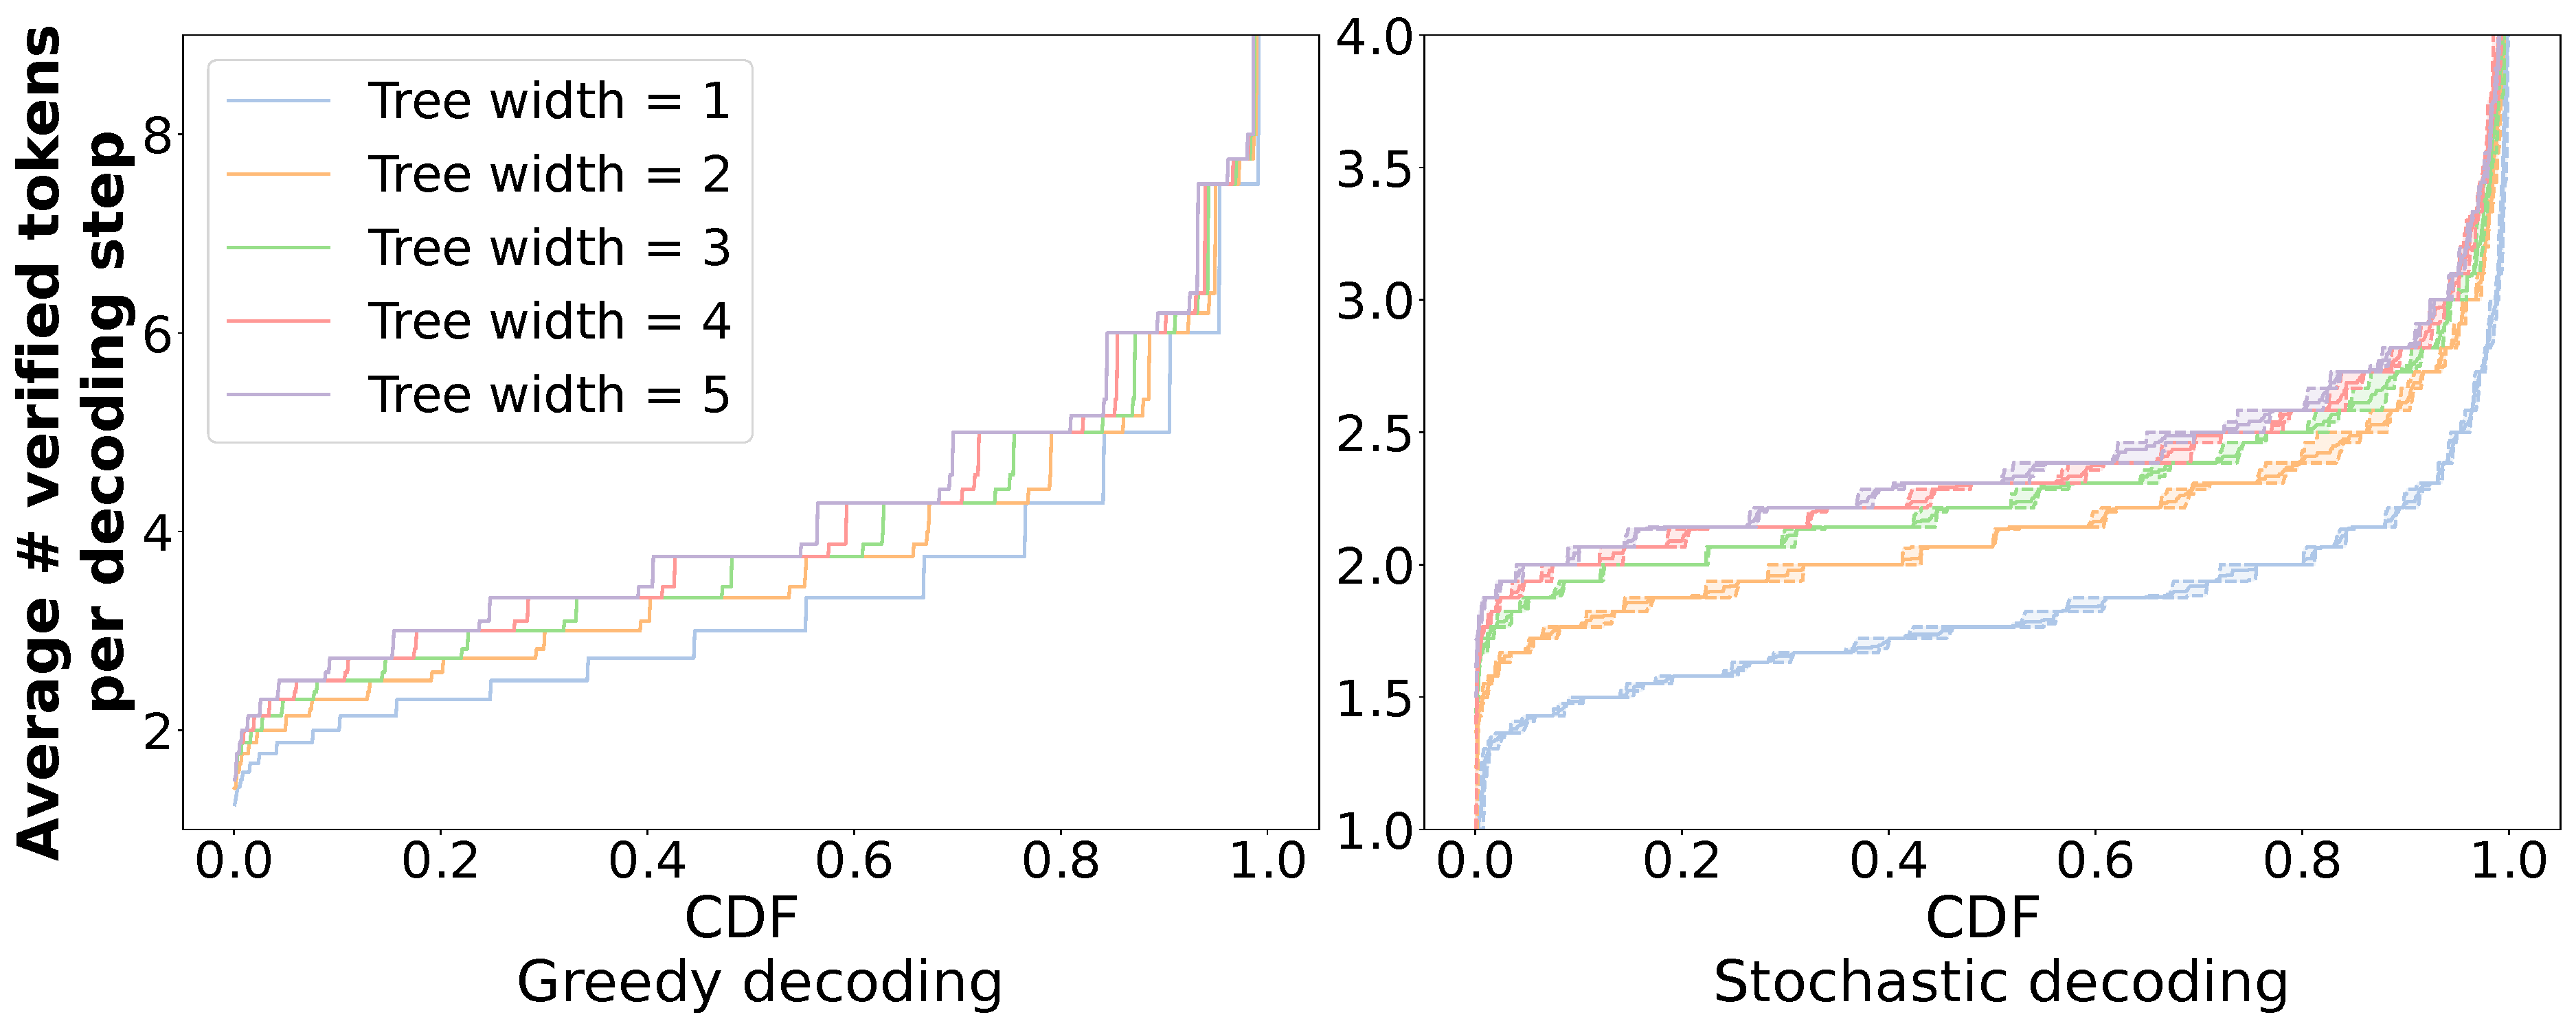
\includegraphics[width=\linewidth]{figs/alpaca_CDF.pdf}
    \caption{\rev{Comparing speculative performance of \sys with different token tree structures.}}
    % \caption{CDF figures of greedy sampling, stochastic sampling and greedy decoding. \ZJ{TODO: (1) increase font size for the y-axis title; (2) change the title to ``Average \# verified tokens per decoding step''; (3) add a ``='' between tree width and value}
    \label{fig:eval_cdf}
\end{figure}

% \if 0
% \begin{table}
% \begin{center}
% % \caption{Average number of tokens verified by \Sys in a decoding step.  We used \llama-7B as the LLM and used different numbers of collectively boost-tuned SSMs, all of which were derived from \llama-160M. The speculation length is 16 for all SSMs.}
% \caption{\ZX {Llama 68M Merge-based token tree (this caption and table label need to be modified).}}
% \footnotesize
% \label{tab:cbt-llama}
% \begin{tabular}{ccccccc}
% \toprule
% \# SSMs  & 1 & 2 & 3 & 4 & 5 \\ \midrule
% Alpaca       & 2.95     & 3.21    & 3.31     & 3.41     & \textbf{3.50}     \\
% CP           & 2.58     & 3.05    & 3.16     & 3.22     & \textbf{3.31}     \\
% WebQA        & 2.27     & 2.42    & 2.58     & 2.65     & \textbf{2.74}     \\
% CIP          & 2.73     & 3.12    & 3.24     & 3.41     & \textbf{3.52}     \\
% PIQA         & 2.18     & 2.44    & 2.54     & 2.62     & \textbf{2.73}         \\ \midrule
% %Avg        &1.34     & 1.39     & 1.60    & 1.67     & 1.73     & \textbf{1.79}      \\ \bottomrule
% \end{tabular}
% \end{center}
% \end{table}
% \fi


\begin{table}
\begin{center}
\caption{\rev{Average number of tokens verified by \sys in a decoding step. We use \llama-7B and \llama-68M as the LLM and SSM, and use different tree widths for constructing a token tree. The speculation length is 8.}}
%\caption{\textcolor{blue}{Llama 68M improved sample (this caption and table label need to be modified).}
%\footnotesize
\label{tab:cbt-llama}

\begin{tabular}{ll|ccccc}
\toprule
& & \multicolumn{5}{c}{{\bf Token tree width}} \\
& Dataset   & 1 & 2 & 3 & 4 & 5 \\ \midrule
\multirow{5}{*}{\rotatebox[origin=c]{90}{\parbox{2cm}{\bf \centering Greedy\\ decoding}}}
& Alpaca     & 2.95     & 3.07    & 3.21     & 3.33     & \textbf{3.43}     \\
& CP         & 2.58     & 3.24    & 3.46     & 3.59     & \textbf{3.69}     \\
& WebQA      & 2.27     & 2.69    & 2.86     & 2.98     & \textbf{3.07}     \\ 
& CIP        & 2.73     & 3.40    & 3.62     & 3.79     & \textbf{3.91}     \\
& PIQA       & 2.18     & 2.80    & 2.97     & 3.10     & \textbf{3.21}     \\  
\midrule
\multirow{5}{*}{\rotatebox[origin=c]{90}{\parbox{2cm}{\bf \centering Stochastic\\ decoding}}}
& Alpaca     & 1.79     & 2.11    & 2.26     & 2.32     & \textbf{2.38}     \\
& CP         & 1.69     & 1.99    & 2.15     & 2.23     & \textbf{2.28}     \\
& WebQA      & 1.64     & 1.93    & 2.08     & 2.15     & \textbf{2.21}     \\
& CIP        & 1.72     & 2.05    & 2.19     & 2.28     & \textbf{2.29}     \\
& PIQA       & 1.67     & 1.93    & 2.08     & 2.15     & \textbf{2.21}         \\ %\midrule
%Avg        &1.64     & 1.70     & 2.00    & 2.15     & 2.23     & \textbf{2.28}      \\ 
\bottomrule
\end{tabular}
\end{center}
\end{table}
%\begin{table}
\caption{Average number of tokens verified by \Sys in a decoding step. We used OPT-13B as the LLM and used different numbers of collectively boost-tuned SSMs, all of which were derived from OPT-125M. The speculation length is 16 for all SSMs.}
\label{tab:cbt-opt}
\begin{center}
\footnotesize
\begin{tabular}{cccccc}
\toprule
               \# SSMs             & 1 & 2 & 3 & 4 & 5 \\ \midrule
CIP & 3.00     & 3.39     & 3.52     & 3.58     & \textbf{3.74}     \\
CP           & 2.95     & 3.35     & 3.49     & 3.52     & \textbf{3.68}     \\
WebQA                      & 2.51     & 2.92     & 3.04     & 3.09     & \textbf{3.20}     \\
Alpaca               & 3.33     & 3.89     & 4.06     & 4.17     & \textbf{4.35}     \\
PIQA                        & 2.75     & 3.14     & 3.26     & 3.31     & \textbf{3.43}     \\ \midrule
Avg                         & 2.91     & 3.34     & 3.47     & 3.53     & \textbf{3.68}     \\ \bottomrule
\end{tabular}
\end{center}
\end{table}


\begin{figure}
    \centering
    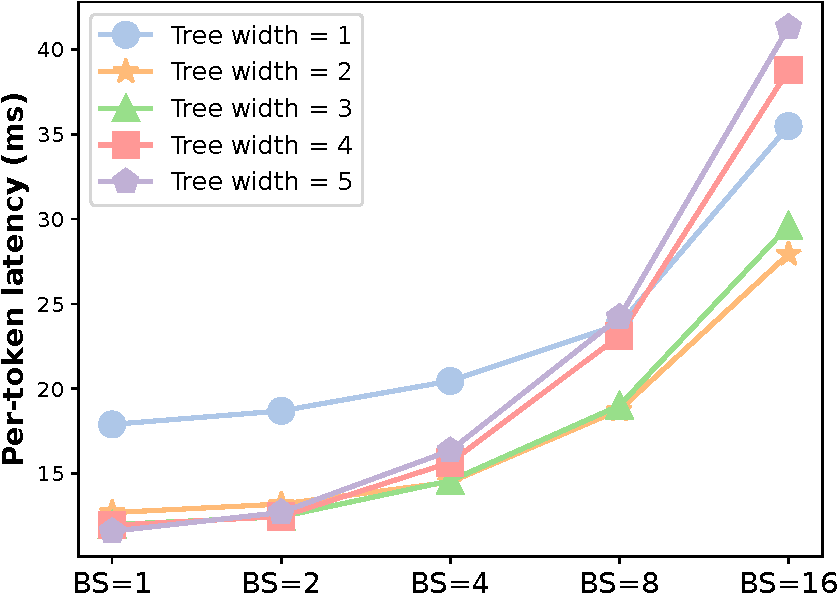
\includegraphics[scale=0.45]{figs/eval_tree_branches-crop.pdf}
    \caption{\rev{\Sys's end-to-end inference latency with different tree widths. We use \llama-7B and \llama-68M as the LLM and SSM.}}
    \label{fig:eval_tree_branches}
\end{figure}

\rev{A larger token tree width reduces the LLM decoding steps to process a request at the cost of increased verification overhead, since \sys must verify more tokens.
\Cref{fig:eval_tree_branches} compares the end-to-end inference latency of \sys using different tree widths.
%
For small batch sizes (i.e., BS = 1 and 2), using a large tree width can consistently reduce per-token latency, since \sys can leverage sparse GPU resources to verify more tokens in parallel while maintaining the same per-iteration latency.
%
For large batch sizes (i.e., BS $\geq 4$), using a large tree width increases the latency to verify a token tree due to less sparse GPU resources that can be leveraged by \sys, and a tree width of $2$ or $3$ achieves the best performance by striking a perfect balance between speculative performance and verification latency.}
%

\if 0
In this section, we evaluate the effectiveness of collective boost-tuning in terms of improving the average number of verified tokens in each LLM decoding step. 
%%%
%For both the OPT and \llama experiments, we fine-tuned four SSMs over the OpenWebText Corpus using collective boost-tuning on top of the pre-trained OPT-125M and \llama-160M models, which provides a collection of five SSMs (including the base SSM) in each experiment.
%%%
As shown in \Cref{tab:cbt-llama}, the average number of tokens verified by \Sys in each LLM decoding step increases consistently across all five datasets due to better alignment between the LLM and our tuned collection of SSMs.
%%%
More specifically, by using collectively boost-tuned SSMs, we have an overall improvement of $26.4\%$ and $22.6\%$ respectively, compared to using only a single pre-trained SSM.

We further study how different numbers of SSMs affect \Sys's inference latency. In this experiment, we use \llama-60B as the LLM and the five collectively boost-tuned \llama-160M models as the SSMs. \Sys uses tensor model parallelism to serve \llama-30B across 4 GPUs and uses data parallelism to serve SSMs on different GPUs. 
%%%
\Cref{fig:eval_ssms} shows the results.
%%%
\Sys's performance is insensitive to the number of SSMs for two reasons.
%%%
First, \Sys uses data parallelism to serve SSMs on different GPUs in parallel. 
As a result, adding more SSMs does not increase the speculation time and marginally increase the verification time (since \Sys needs to verify more tokens).
Second, as shown in \XM{\Cref{tab:cbt-opt}} and~\Cref{tab:cbt-llama}, the first several SSMs are critical to achieving high speculative performance and the average matching length increases slightly (i.e., from 3.27 to 3.58 and from 3.34 to 3.68 for OPT and \llama) as we introduce more SSMs. \XM{TODO: update}
\fi 

% \begin{figure}[H]
%     \centering
%     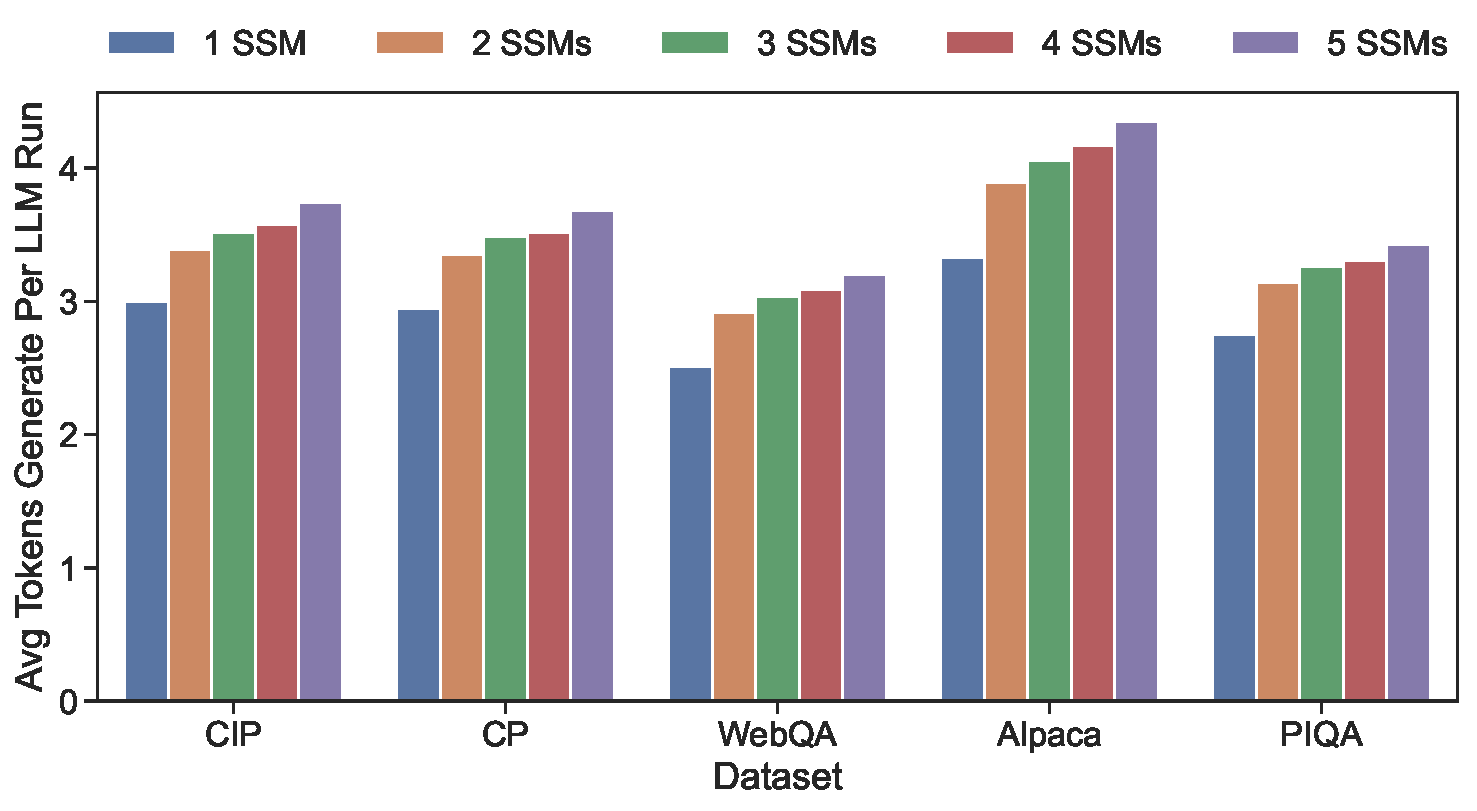
\includegraphics[width=\columnwidth]{figs/CBT-OPT.pdf}
%     \caption{Average number of tokens verified by \Sys in each LLM decoding step over five datasets. We use a fixed speculation length of 16 for all the SSMs in this experiment. We used OPT-13B as the LLM and used four SSMs boost-tuned from OPT-125M.}
%     \label{fig:CBT-OPT}
% \end{figure}


% \begin{figure}[H]
%     \centering
%     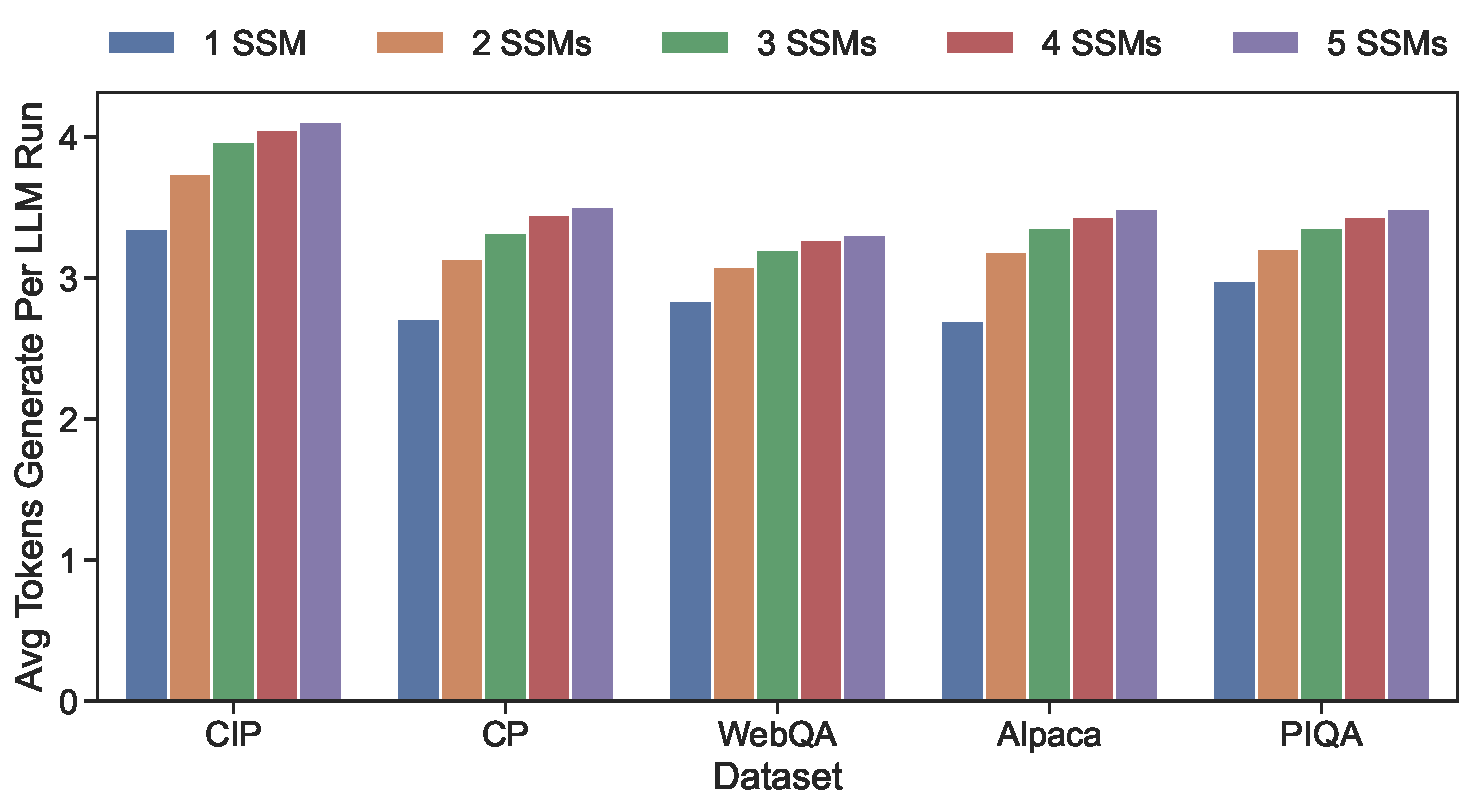
\includegraphics[width=\columnwidth]{figs/CBT-LLaMA.pdf}
%     \caption{Average number of tokens verified by \Sys in each LLM decoding step over five datasets. We use a fixed speculation length of 16 for all the SSMs in this experiment. We used \llama-7B as the LLM and used four SSMs boost-tuned from \llama-160M.}
%     \label{fig:CBT-LLaMA}
% \end{figure}

\if 0
\subsection{Learning-based Speculative Scheduler}
\label{subsec:eval_scheduler}
\ZJ{We will be removing the learning-based scheduler part right?}
For the learning-based speculative scheduler, we demonstrate some preliminary results on the matching length predictor in this section.
%%%
We use a three-layer MLP with a hidden feature size of 64 as our predictor.
%%%
We train the predictor on 200K samples over the OpenWebText corpus.
%%%
The labels are generated using OPT-13B as the LLM and OPT-125M as the SSM.
%%%
As shown in~\Cref{tab:lss-opt}, using the predictor can achieve similar LLM runs while reducing the SSM runs significantly due to dynamic speculation length. 
Nevertheless, there is still plenty of space to improve the predictor as the optimal SSM run would be the average matching length times the LLM run.

%%%
% \if 0
% \begin{table}[H]
% \caption{\XM{TODO: add a caption}}
% \label{tab:lss-opt}
% \begin{center}
% \begin{tabular}{ccccccccccc}
% \hline
%         & \multicolumn{2}{c}{CIP} & \multicolumn{2}{c}{CP} & \multicolumn{2}{c}{WebQA} & \multicolumn{2}{c}{Alpaca} & \multicolumn{2}{c}{PIQA} \\ \cline{2-11} 
%         & w/ oracle  & w/o oracle & w/ oracle & w/o oracle & w/ oracle   & w/o oracle  & w/ oracle   & w/o oracle   & w/ oracle  & w/o oracle  \\ \hline
% LLM Run & 8812       & 8449       & 3625      & 3462       & 12624       & 12080       & 11123       & 10684        & 12625      & 11560       \\
% SSM Run & 56401      & 135184     & 23172     & 55392      & 74953       & 193280      & 72863       & 170944       & 74548      & 184960      \\ \hline
% \end{tabular}
% \end{center}

% \end{table}

\begin{table}
\caption{The number of LLM runs and SSM runs with or without the presence of the matching length predictor. When there is no predictor, we use a fixed speculation length of 16 for all the SSMs in this experiment. LLM: OPT-13B, SSMs: OPT-125M}
\label{tab:lss-opt}
\begin{center}
\begin{tabular}{ccccc}
\toprule
       & \multicolumn{2}{c}{LLM run} & \multicolumn{2}{c}{SSM run} \\ \cmidrule{2-5} 
       & w/ predictor    & w/o predictor   & w/ predictor    & w/o predictor   \\ \midrule
CIP    & 8812         & 8449         & 56401        & 135184       \\
CP     & 3625         & 3462         & 23172        & 55392        \\
WebQA  & 12624        & 12080        & 74953        & 193280       \\
 Alpaca & 11123        & 10684        & 72863        & 170944       \\
PIQA   & 12625        & 11560        & 74548        & 184960       \\ \bottomrule
\end{tabular}
\end{center}
\end{table}
% \fi 
%%%
\fi

\subsection{\rev{Tree-based Parallel Decoding}}
\label{subsec:eval_tree_based_decoding}

\begin{figure}
    \centering
    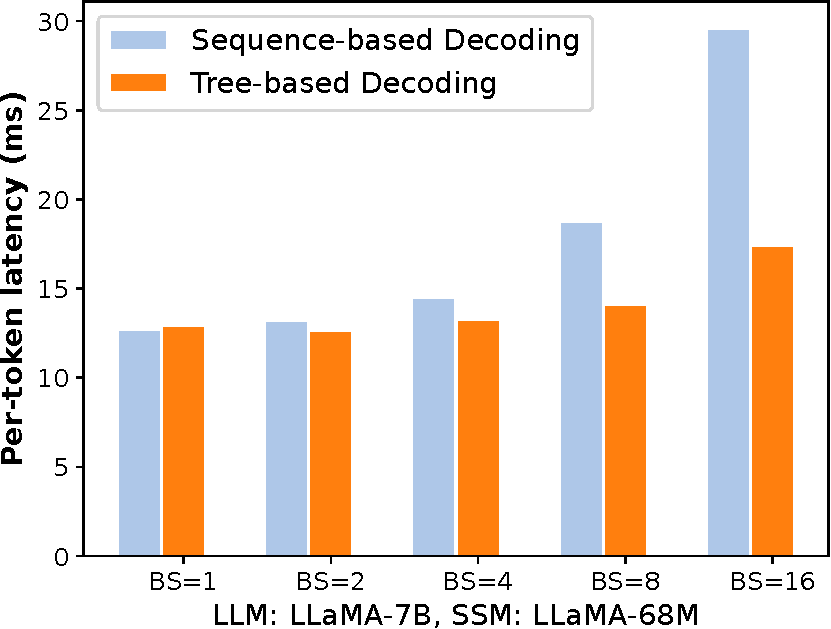
\includegraphics[scale=0.45]{figs/tree-based-decoding-crop.pdf}
    \caption{\rev{Comparing \Sys's tree-based parallel decoding with the sequence-based decoding mechanism employed by existing LLM inference systems.}}
    %\vspace{-4mm}
    \label{fig:eval_tree_based_decoding}
\end{figure}

\rev{We now evaluate the effectiveness of \sys's tree-based parallel decoding mechanism, which decodes all tokens of a token tree in parallel.
%
As a comparison, all existing LLM inference systems use sequence-based decoding, which requires decomposing a token tree into multiple sequences of tokens and processing these sequences using separate resources due to potential key-value cache conflicts (see \S\ref{subsec:optimization}).
%
% \Cref{fig:eval_tree_based_decoding} shows a comparison between the two methods. 
As shown in \Cref{fig:eval_tree_based_decoding}, \sys's tree-based parallel decoding achieves on-par performance as existing sequence-based decoding mechanism for small batch sizes and outperforms it by up to 1.8$\times$ for large batch sizes. The improvement is realized by (1) eliminating redundant attention computation for sequences with a shared prefix, and (2) fusing tree attention of all tokens in a single kernel through the topology-aware casual mask (see \S\ref{subsec:optimization}).}

\begin{table}
\begin{center}
\caption{\rev{Average number of tokens verified by \sys in a stochastic decoding step with different sampling algorithms. We use \llama-7B and \llama-68M as the LLM and SSM. Each token tree has a width of 5 and a depth of 8.}}
%\caption{\textcolor{blue}{Llama 68M improved sample (this caption and table label need to be modified).}
\label{tab:eval_msss}
\resizebox{\linewidth}{!}{%
\begin{tabular}{l|rrr}
\toprule
& {\bf Naive}  & {\bf Multi-Step} & {\bf Improvement} \\ 
& {\bf Sampling} & {\bf Spec. Sampling} & \\ \midrule
Alpaca     & 1.87     & 2.38    & 1.27$\times$\\
CP         & 1.80     & 2.28    & 1.26$\times$\\
WebQA      & 1.73     & 2.21    & 1.28$\times$\\ 
CIP        & 1.79     & 2.29    & 1.28$\times$\\
PIQA       & 1.73     & 2.21    & 1.28$\times$\\  
\bottomrule
\end{tabular}%
}
\end{center}
\end{table}

\subsection{\rev{Multi-Step Speculative Sampling}}
\label{subsec:eval_msss}


\rev{This section evaluates how our multi-step speculative sampling (MSS) and the \textproc{VerifyStochastic} algorithm improves the speculative performance of \sys when performing stochastic decoding.
%
We use naive sampling as a baseline where \sys directly samples the next token from the LLM and examines whether the sampled token is included in the speculated token tree (see \S\ref{subsec:verification}).
%
Since different sampling algorithms involve identical speculation and verification overheads, we focus on the average number of tokens that can be verified in each stochastic decoding step in this experiment.
%
\Cref{tab:eval_msss} shows the results. Compared to naive sampling, MSS can consistently improve the number of verified tokens by 1.2-1.3$\times$ on average across a variety of prompt datasets, while guaranteeing the same output distribution with the LLM.
%
}
\section{Related Work}
\label{sec:related}

Transformer-based LLMs have demonstrated significant potential in numerous human-level language modeling tasks by continuously increasing their sizes~\cite{vaswani2017attention, rae2021scaling, smith2022using, du2022glam, chowdhery2022palm}.
%%%
As GPT-3 becomes the first model to surpass 100B parameters~\cite{brown2020language}, multiple LLMs ($>$100B) have been released, including OPT-175B~\cite{zhang2022opt}, Bloom-176B~\cite{scao2022bloom}, and PaLM~\cite{chowdhery2022palm}.
%%%
%Due to the auto-regressive nature of LLMs and their humongous model size, inference latency can be non-negligible in practice. 
%%%
Recent work has proposed a variety of approaches to accelerating generative LLM inference, which can be categorized into two classes.

\paragraph{Lossless acceleration.}
Prior work has explored the idea of using an LLM as a verifier instead of a decoder to boost inference.
%%%
For example, Yang et al.~\cite{yang2023inference} introduced {\em inference with reference}, which leverages the overlap between an LLM's output and the references obtained by retrieving documents, and checks each reference's appropriateness by examining the decoding results of the LLM.
Motivated by the idea of speculative execution in processor optimizations~\cite{burton1985speculative, hennessy2011computer}, recent work proposed {\em speculative decoding}, which uses a small language model to produce a sequence of tokens and examines the correctness of these tokens using an LLM~\cite{leviathan2022fast, xiaspeculative, stern2018blockwise, chen2023accelerating, gante2023assisted}.
%%%
There are two key differences between \Sys and these prior works.
First, instead of only considering a single sequence of tokens, \Sys generates and verifies a token tree, whose nodes each represent a unique token sequence. \Sys performs tree attention to compute the attention output of these token sequences in parallel and uses a novel tree-based decoding algorithm to reuse intermediate results shared across these sequences.
%%%
Second, prior attempts generally consider a single small language model for speculation, which cannot align well with an LLM due to the model capacity gap between them.
%%%
\rev{\Sys introduces two novel speculation methods, including 1) expanding from a single SSM and 2) merging from multiple fine-tuned SSMs, and the generated token tree largely increases the coverage of the LLM's output.}
% \Sys introduces collective boost-tuning to adapt different SSMs to align with an LLM under different scenarios, which largely increases the coverage of the speculated token trees produced by \Sys.
%Third, an additional challenge \Sys has to address is deciding the speculative configuration for a given request. \Sys leverages an important observation that the tokens generated by an LLM involve diverse difficulties to speculate, and uses a learning-based speculator to decide which SSMs to use and their speculative configurations.

Prior work has also introduced a variety of techniques to optimize ML computations on modern hardware platforms. 
%%%
For example, TVM~\cite{chen2018tvm} and Ansor~\cite{zheng2020ansor} automatically generate kernels for a given tensor program. TASO~\cite{jia2019taso} and PET~\cite{wang2021pet} automatically discover graph-level transformations to optimize the computation graph of a DNN.
\Sys's techniques are orthogonal and can be combined with these systems to accelerate generative LLM computation, which we believe is a promising avenue for future work.

% \ZJ{ZZ's original version:}
% In order to preserve output equivalency while reducing inference latency, \cite{leviathan2022fast, yang2023inference, xiaspeculative, stern2018blockwise, chen2023accelerating} bring the idea of speculative execution in processor optimizations~\cite{burton1985speculative, hennessy2011computer} to LLM inference optimization. 
% %%%
% Instead of solely relying on the LLM for inference, this line of work uses cheaper and faster proxies to do speculations followed by a verification procedure using the slower LLM to preserve equivalency.
% %%%
% Nevertheless, the quality of the speculation proxies as well as the system optimization opportunities for the verification process have been underexplored, which are the key focuses of this work.  


\paragraph{Lossy acceleration.}
BiLD~\cite{biglittletransformer} is a speculative decoding framework that uses a single SSM to accelerate LLM decoding. Unlike the systems mentioned above, the acceleration is lossy: speed comes at the cost of a possible degradation in the generated tokens. 
Another line of research leverages model compression to reduce LLM inference latency while compromising the predictive performance of the LLM.
%%%
% To this end, recent works have introduced a variety of techniques to reduce the end-to-end latency of serving LLMs. 
%%%
For example, prior work proposed to leverage weight/activation quantization of LLMs to reduce the memory and computation requirements of serving these LLMs~\cite{xiao2022smoothquant, frantar2023gptq, park2022nuqmm, yao2022zeroquant,dettmers2022gpt3}.
%%%
Recent work further explores a variety of structured pruning techniques for accelerating Transformer-based architectures~\cite{frantar2023sparsegpt, wang2021spatten, hubara2021accelerated}.
%%%
%Regardless, few of them have been used in practice due to unpredictable performance degradation. 
%%%
A key difference between \Sys and these prior works is that \Sys does not directly reduce the computation requirement for performing LLM inference, but instead reorganizing LLM inference computation in a more parallelizable way, which reduces memory accesses and inference latency at the cost of manageable memory and computation overheads.

\paragraph{Tree-structured attention.}
%Prior work by Nguyen et al.~\cite{Nguyen2020} introduced {\em tree-structured attention} , a technique to let a Transformer model capture the hierarchical composition of the input text by running the model on the text's parse tree. The key idea is to use a one-on-one mapping called {\em hierarchical accumulation}, to encode the parse tree in a form that can be processed by the attention, and then decode it back into tree form.
%%%
%There are two key difference between the tree-structured attention and \sys's tree-based decoding mechanism. First, \sys employs a tree structure to combine multiple candidate sequences together so as to condense identical prefixes; whereas Nguyen et al. represent a single input sequence using its parse tree. \sys does not attempt to incorporate into the LLM model additional information about each input sequence's structure, but rather, it accelerates LLM inference by verifying multiple decoded sequences (each generated by a SSM) in parallel. Second, unlike in the work by Nguyen et al., \sys's attention does not output another tree object, but rather, a single sequence of tokens.
Nguyen et al.~\cite{Nguyen2020} introduced {\em tree-structured attention}, a technique that lets a Transformer model capture the hierarchical composition of input text by running the model on the text's parse tree. To process with attention, it uses a one-on-one mapping to encode and decode the tree.
% , so that the attention can process it. 
There are two key differences from \sys's tree-based decoding. First, \sys uses a tree to combine candidate sequences to condense prefixes, whereas Nguyen et al. represent a single sequence with its parse tree. \sys does not incorporate parse tree into the LLM, but accelerates inference by verifying decoded sequences in parallel. Second, \sys's attention outputs a token sequence, not a tree.

\paragraph{Multi-sample decoding techniques}
% Like tree-based speculative inference, multi-sample decoding techniques such as \textit{beam search}, \textit{top-k sampling}, and \textit{top-p sampling} consider multiple candidate token sequences or next tokens at each step, rather than just the single highest probability option. They can also prune or ignore low probability sequences or tokens. There are two key differences from \sys's tree-based decoding. First, tree-based decoding in \sys is used to speculatively predict and verify multiple candidate token sequences in parallel against a large language model (LLM). The goal is to reduce latency by decreasing the number of decoding iterations needed. Beam search and top-k/top-p sampling are used during the decoding process to generate high-probability token sequences. They do not decrease the number of decoding steps.  Second, tree-based decoding leverages small speculative models (SSMs) to predict candidate sequences verified in parallel against the LLM. Beam search and top-k/top-p sampling are decoding strategies applied directly to the probability distribution over next tokens provided by the LLM itself.
% Overall, beam search, top-k sampling, and top-p sampling are decoding optimizations that are orthogonal to the techniques proposed in this paper. \sys supports using these techniques, which can be combined with tree-based speculative decoding.
Like tree-based speculative inference, \textit{beam search}, \textit{top-k sampling}, and \textit{top-p sampling} consider multiple candidate token sequences at each step and can prune low-probability options. However, tree-based decoding in \sys speculatively predicts and verifies multiple candidates in parallel against an LLM to reduce decoding iterations and latency, leveraging small speculative models (SSMs). In contrast, beam search and top-k/top-p sampling are decoding strategies applied directly to the LLM's output probabilities to generate high-probability sequences without reducing decoding steps. \sys supports beam search, top-k sampling, and top-p sampling. These techniques are orthogonal decoding optimizations and can be combined with tree-based speculative decoding.
 

\section{Conclusion}
This paper introduces \Sys, a system that accelerates generative LLM inference with tree-based speculative inference and verification.
A key insight behind \Sys is to simultaneously consider a diversity of speculation candidates to efficiently predict the LLM’s outputs, which are organized as a token tree and verified against the LLM in parallel using a tree-based parallel decoding mechanism.
% A key insight behind \Sys is to combine multiple small speculative models to efficiently predict the LLM’s outputs, which are organized as a token tree and verified against the LLM in parallel using a tree-based parallel decoding mechanism.
\Sys significantly reduces the memory accesses to the LLM's parameters and the end-to-end LLM inference latency for both distributed and offloading-based LLM inference.

\iffinal
\section*{Acknowledgement}
We thank Tianqi Chen, Bohan Hou, Hongyi Jin, the anonymous ASPLOS reviewers, and our shepherd Shan Lu for their feedback on this work. This research is partially supported by NSF awards CNS-2147909, CNS-2211882, and CNS-2239351, and research awards from Amazon, Cisco, Google, Meta, Oracle, Qualcomm, and Samsung. 
\fi 


\appendix
\section{Artifact Appendix}

%%%%%%%%%%%%%%%%%%%%%%%%%%%%%%%%%%%%%%%%%%%%%%%%%%%%%%%%%%%%%%%%%%%%%
\subsection{Abstract}

% {\em Obligatory}
The artifact contains the code to run \sys, as well as the datasets and scripts that can be used to reproduce the experiments in the paper. 
\subsection{Artifact check-list (meta-information)}

% {\em Obligatory. Use just a few informal keywords in all fields applicable to your artifacts
% and remove the rest. This information is needed to find appropriate reviewers and gradually 
% unify artifact meta information in Digital Libraries.}

{\small
\begin{itemize}
  \item {\bf Algorithm: } Tree-based Speculative Inference
  \item {\bf Program: } spec\_infer.cc, incr\_decoding.cc
  \item {\bf Compilation: } CMake
  % \item {\bf Transformations: }
  % \item {\bf Binary: }
  % \item {\bf Model: }
  % \item {\bf Data set: } LLAMA, OPT models
  \item {\bf Run-time environment: } CUDA, NCCL, MPI, UCX, Python3.
  \item {\bf Hardware: }  Two AWS g5.12xlarge instances, each with 4 NVIDIA A10 24GB GPUs, 48 CPU cores, and 192 GB DRAM.
  % \item {\bf Run-time state: }
  % \item {\bf Execution: }
  \item {\bf Metrics: } End to-end average latency
  \item {\bf Output: } End-to-end latency
  \item {\bf Experiments: } Server-grade GPU inference, Offloading-based inference
  \item {\bf How much disk space required (approximately)?: } 350GB per node
  \item {\bf How much time is needed to prepare workflow (approximately)?: } 2h
  \item {\bf How much time is needed to complete experiments (approximately)?: } 6h
  \item {\bf Publicly available?: } Yes
  \item {\bf Code licenses (if publicly available)?: } Apache License v2.0
  \item {\bf Data licenses (if publicly available)?: } LLAMA is under the GNU license and OPT is under a Non-commercial license%, see \url{https://github.com/facebookresearch/metaseq/blob/main/projects/OPT/MODEL_LICENSE.md}
  \item {\bf Archived (provide DOI)?: }\url{https://doi.org/10.5281/zenodo.10854410}.
\end{itemize}
}

%%%%%%%%%%%%%%%%%%%%%%%%%%%%%%%%%%%%%%%%%%%%%%%%%%%%%%%%%%%%%%%%%%%%%
\subsection{Description}

\subsubsection{How to access}
% {\em Obligatory}
The artifact is released on Github: \url{https://github.com/goliaro/specinfer-ae}. The repository contains \sys's source code, and the instructions to build the framework. We also provide scripts to reproduce the experiments from the paper. To clone the repository, use the following command (make sure to pass the \texttt{--recursive} flag):
\begin{lstlisting}[language=sh]
git clone --recursive \
https://github.com/goliaro/specinfer-ae.git
\end{lstlisting}

\subsubsection{Hardware dependencies}
We run out experiments on two AWS g5.12xlarge instances, each with 4 NVIDIA A10 24GB GPUs, 48 CPU cores, and 192 GB DRAM. We provide instructions to create and setup the instances. 
%We will also give the reviewers login access to two pre-configured instances in our own AWS EC2 account. 

\subsubsection{Software dependencies}
The following software is required: CUDA 12.1, NCCL, Rust, CMake and Python3. Further, UCX and MPI are required for the multinode experiments. Additional Python dependencies are listed here: \url{https://github.com/flexflow/FlexFlow/blob/inference/requirements.txt}. We recommend using the \texttt{Deep Learning OSS Nvidia Driver AMI GPU PyTorch 2.1.0 (Ubuntu 20.04)} AMI, and provide scripts and a conda environment to install all the remaining dependencies.

% \subsubsection{Data sets}

\subsubsection{Models}
We use the following LLM/SSM models for our experiments (for each model, we specify in parentheses the corresponding HuggingFace repository): LLaMA-68M (JackFram/llama-68m), LLaMA-7B (huggyllama/llama-7b), LLaMA-65B (huggyllama/llama-65b), OPT-125M (facebook/opt-125m), OPT-13B (facebook/opt-13b), OPT-125M (facebook/opt-30b). You can download all these models with the script: 
\begin{lstlisting}[language=sh]
./download_models.sh
\end{lstlisting}

%%%%%%%%%%%%%%%%%%%%%%%%%%%%%%%%%%%%%%%%%%%%%%%%%%%%%%%%%%%%%%%%%%%%%
\subsection{Installation}

% {\em Obligatory}

To reproduce the experiments, you will need access to two AWS g5.12xlarge instances (or other machines with the same GPU/CPU/network specs). If you are using the preconfigured instances we provided, you can skip this step. 
\paragraph{Launching the instances}
Launch two AWS g5.12xlarge instances using the \texttt{Deep Learning OSS Nvidia Driver AMI GPU PyTorch 2.1.0 (Ubuntu 20.04)} AMI. Make sure to place the instances in a \href{https://docs.aws.amazon.com/AWSEC2/latest/UserGuide/placement-groups.html}{placement group} that utilizes the cluster strategy to achieve low-latency network performance. Attach the same security group to all instances and add an inbound rule in the security group to allow all incoming traffic from the same security group. For example, you can add the following rule: Type: All TCP, Source: Anywhere-IPv4.

\paragraph{Installing the prerequisites}
After gaining access to the AWS instances, install the prerequisites by following the steps below. First, activate the conda shell support by running \texttt{conda init bash}, and then restarting the shell session.
Next, create the conda environment with all the required dependencies by running:
\begin{lstlisting}[language=sh]
conda env create -f FlexFlow/conda/flexflow.yml
conda activate flexflow
\end{lstlisting}

\paragraph{Multinode setup}
Download and build UCX by running the \texttt{install\_ucx.sh} script. Next, if you are running \sys on two AWS instances, you will need to configure MPI so that the two instances are mutually accessible. Pick a main node, and create a SSH key pair with:
\begin{lstlisting}[language=sh]
    ssh-keygen -t ed25519
\end{lstlisting}
Append the contents of the public key (\texttt{\textasciitilde/.ssh/id\_ed25519.pub}) to the \texttt{\textasciitilde/.ssh/authorized\_keys} file on BOTH the main and secondary machine. Note that if the \texttt{.ssh} folder or the \texttt{authorized\_keys} file do not exist, you will need to create them manually. 
Finally, create a file at the path \texttt{\textasciitilde/hostfile} with the following contents:
\begin{lstlisting}[language=sh]
<main_node_private_ip> slots=4
<secondary_node_private_ip> slots=4
\end{lstlisting}
replacing <main\_node\_private\_ip> and <secondary\_node\_private\_ip> with the private IP addresses of the two machines, and the number of slots with the number of GPUs available (if you are using the recommended AWS instances, you will use a value of 4). You can find each machine's private IP address by running the command (and use the first IP value that is printed):
\begin{lstlisting}[language=sh]
    hostname -I
\end{lstlisting}

\paragraph{Install \sys}

To install \sys, run the script: 
\begin{lstlisting}[language=sh]
./install_specinfer.sh
\end{lstlisting}

\subsection{Basic Test}
To ensure that \sys is installed correctly and is functional, run the \texttt{basic\_test.sh} script. This script will test the basic incremental decoding and speculative inference functionalities, on both single and multi nodes. It will also test the support for offloading. The test passes if it prints the "Test passed!" message. 

%%%%%%%%%%%%%%%%%%%%%%%%%%%%%%%%%%%%%%%%%%%%%%%%%%%%%%%%%%%%%%%%%%%%%
\subsection{Experiment workflow}
The artifact comes with scripts to gather the data that can be used to reproduce the results from the paper. It also comes with scripts that can be used to convert the output data into CSV format for plotting. 

\paragraph{Running Experiments}
We run the following two experiments to evaluate \sys under different hardware setups. The output data will be saved to the \texttt{FlexFlow/inference/output} path. 

\begin{itemize}
    \item \textbf{Server-grade GPU evaluation.} This experiment tests the performance of \sys on server-grade GPUs. The LLMs and SSMs are loaded in GPU memory, and we measure the end-to-end inference latency using 1 node, and 2 nodes. In the single node case, we measure the performance using 1 GPU, or 4 GPUs. In the multinode case, we use 4GPUs per node. The experiments use LLAMA-7B, OPT-30B and LLAMA-65B as the LLMs, and LLAMA-68M and OPT-125M as SSMs. The experiment runs \sys in three different modes: incremental decoding, sequence-based speculative decoding, and tree-based speculative decoding. The former two are used to obtain data for the ablation study, and the latter is the novel inference mode proposed by \sys, and will be deployed by the user. To run the server-grade GPU evaluation, run:
\begin{lstlisting}[language=sh]
./server_gpu_experiments.sh
\end{lstlisting}
\item \textbf{Offloading evaluation.} This experiment tests the performance of \sys when loading only a subset of parameters in GPU memory, while offloading the remaining ones on CPU DRAM. This technique is used to perform inference when the target model is larger than the available GPU memory. In the experiment, \sys uses a single GPU and swaps the model's weights to and from the CPU. To run the offloading evaluation, run: 
\begin{lstlisting}[language=sh]
./offloading_experiments.sh
\end{lstlisting}
\end{itemize}

\paragraph{Third-party frameworks}
Please follow the vLLM, FasterTransformer, and HuggingFace TGI, and FlexGen official documentation to reproduce the performance of the third-party frameworks under the experiment scenarios.

\paragraph{Output data}
The scripts above will generate data at the \texttt{FlexFlow/inference/output} path. For each scenario, a \texttt{.txt} file contains the generated output for each prompt, and a \texttt{.out} file contains the stdout logs. The quality of the generated output can be evaluated visually and compared with the output from third-party inference frameworks.
We provide scripts to parse the raw output data and generate CSV files that can be used to generate the paper's figures. The README provides all details on the scripts and the mapping between CSV files and figures.

%%%%%%%%%%%%%%%%%%%%%%%%%%%%%%%%%%%%%%%%%%%%%%%%%%%%%%%%%%%%%%%%%%%%%
\subsection{Evaluation and expected results}
The data from the CSV files should show similar performance to the figures from the paper. Some variability is to be expected, but overall, \sys should behave according to Figures 7-11 from the paper. 
% {\em Obligatory}

%%%%%%%%%%%%%%%%%%%%%%%%%%%%%%%%%%%%%%%%%%%%%%%%%%%%%%%%%%%%%%%%%%%%%
\subsection{Experiment customization}
Users can edit the configuration parameters from the evaluation scripts to change various parameters, such as the number of GPUs/CPUs, GPU/CPU memory, batch size, LLM/SSM models used, prompt dataset, full vs. half-precision, and the maximum number of tokens to generate.

%%%%%%%%%%%%%%%%%%%%%%%%%%%%%%%%%%%%%%%%%%%%%%%%%%%%%%%%%%%%%%%%%%%%%
% \subsection{Notes}
% \section{Appendix}

\begin{table}[h]
\begin{center}
\caption{\rev{Average number of tokens verified by \sys in a greedy decoding step with the merge- and expansion-based token tree construction methods. We used \llama-7B and \llama-68M as the LLM and SSM, respectively. Each speculated token tree has a depth of 8.
%\ZX {Why the depth is 8? In our experiments, I think it is 16.} \ZJ{I used 8 for all the other experiments and thought it's also 8 for yours.}.
}}
%\caption{\textcolor{blue}{Llama 68M improved sample (this caption and table label need to be modified).}
\label{tab:eval_tree_construction_methods}
%\resizebox{\linewidth}{!}{%
\begin{tabular}{cc|ccc}
\toprule
{\bf Dataset} & {\bf Tree Width} & {\bf Merge}  & {\bf Expansion} & {\bf Diff.} \\ 
 & {\bf / \# SSMs} & & & \\ \midrule
%& {\bf Sampling} & {\bf Spec. Sampling} & \\ \midrule
\multirow{5}{*}{Alpaca}  & 1  & 2.95     & 2.95    & 0\\
  & 2  & 3.21     & 3.07    & $\downarrow$ 0.14\\
  & 3  & 3.31     & 3.27    & $\downarrow$ 0.04\\
  & 4  & 3.41     & 3.33    & $\downarrow$ 0.08\\
  & 5  & 3.51     & 3.43    & $\downarrow$ 0.08\\
\midrule
\multirow{5}{*}{CP}  & 1  & 2.58     & 2.58    & 0\\
  & 2  & 3.05     & 3.24    & $\uparrow$ 0.19\\
  & 3  & 3.16     & 3.46    & $\uparrow$ 0.30\\
  & 4  & 3.22     & 3.59    & $\uparrow$ 0.37\\
  & 5  & 3.31     & 3.69    & $\uparrow$ 0.38\\
\midrule
\multirow{5}{*}{WebQA}  & 1  & 2.27     & 2.27    & 0\\
  & 2  & 2.42     & 2.69    & $\uparrow$ 0.27\\
  & 3  & 2.58     & 2.86    & $\uparrow$ 0.28\\
  & 4  & 2.65     & 2.98    & $\uparrow$ 0.33\\
  & 5  & 2.74     & 3.07    & $\uparrow$ 0.33\\
\midrule
\multirow{5}{*}{CIP}  & 1  & 2.73     & 2.73    & 0\\
  & 2  & 3.12     & 3.40    & $\uparrow$ 0.28\\
  & 3  & 3.24     & 3.62    & $\uparrow$ 0.28\\
  & 4  & 3.41     & 3.79    & $\uparrow$ 0.38\\
  & 5  & 3.52     & 3.91    & $\uparrow$ 0.39\\
\midrule
\multirow{5}{*}{PIQA}  & 1  & 2.18     & 2.18    & 0\\
  & 2  & 2.44     & 2.80    & $\uparrow$ 0.36\\
  & 3  & 2.54     & 2.97    & $\uparrow$ 0.37\\
  & 4  & 2.62     & 3.10    & $\uparrow$ 0.48\\
  & 5  & 2.73     & 3.21    & $\uparrow$ 0.48\\
\bottomrule
\end{tabular}%
%}
\end{center}
\end{table}

\subsection{Comparing Tree Construction Methods}
\label{sec:eval_tree_construction_methods}

\rev{This section compares the expansion- and merged-based tree construction methods used in \Sys.
%
Since the two methods use the same approach to generating speculative tokens from SSMs and verifying a token tree using an LLM, their performance difference only comes from using different methods for constructing token trees.
%
Therefore, our evaluation focuses on the speculative performance of the two methods under the same speculation budget, which is quantified by the tree width for the expansion-based method and the number of SSMs for the merge-based method.
%
\Cref{tab:eval_tree_construction_methods} shows the results. 
When the tree width (and the number of SSMs) is equal to 1, the two methods generate identical speculated token trees (i.e., a sequence of tokens) and achieve the same speculative performance.
%
For larger speculation budgets, the expansion-based method achieves slightly worse performance than the merge-based one for the Alpaca dataset and largely outperforms it for all other datasets in our evaluation.
}

\subsection{Collective Boost-tuning Methodology}
\label{sec:cbt_method}
We didn't find a publicly available pre-trained version of small \llama models, and therefore trained a \llama-68M from scratch for one epoch using the Wikipedia dataset~\cite{wikidump} and part of the C4 dataset~\cite{2019t5}, which took approximately 275 hours on a single NVIDIA A100 GPU.
%%%
We also used the OpenWebText Corpus~\cite{Gokaslan2019OpenWeb} to collectively boost-tune multiple SSMs for speculative inference.
Note that we only need to pre-train and collectively boost-tune SSMs once for each LLM model family before serving. 
For both the OPT and \llama experiments, we fine-tuned four SSMs over the OpenWebText Corpus using collective boost-tuning on top of the pre-trained OPT-125M and \llama-160M models, which provides a collection of five SSMs (including the base SSM).
%\XM{Thinking to move boost-tuning to appendix}



\subsection{Proof of the Theorems}
\label{sec:appendix}
\begin{theorem}
%\label{thm:stochastic_sampling}
For a given $LLM$ and $m$ SSMs (i.e., $SSM_1$,...,$SSM_m$, let $P(u_i | U; \Theta_{LLM})$ be the probability distribution of sampling a token using stochastic sampling, where $U = u_0,...,u_{i-1}$ are previously generated tokens, $u_i$ is the next token to generate, $\Theta_{LLM}$ represents the parameterized LLM. Let $P_{rm{\Sys}}(u_i | U; \Theta_{LLM}, \{\Theta_{SSM_j}\})$ be the probability distribution of sampling token $u_i$ using \Sys's multi-step speculative sampling (see the $\textproc{VerifyStochastic}$ function in \Cref{alg2}), where $\Theta_{SSM_j}$ is the $j$-th parameterized SSM. Then $ \forall U, u_i, \Theta_{LLM}, \Theta_{SSM_j}$ we have
\begin{eqnarray}
P(u_i \mid U; \Theta_{LLM}) = P_{\rm{\Sys}}(u_i \mid U; \Theta_{LLM}, \{\Theta_{SSM_j}\})
\end{eqnarray}
\end{theorem}

%we design a generalized speculative sampling procedure that guarantees the equivalency of the sampling distribution of LLM while maximizing the number of generated tokens per verification step, as shown in~\Cref{alg:gss}. We further present the equivalency proof below.
%%%
\begin{proof}
It suffices to prove the equivalency for a single decoding step.
Let $u_{i-1}$ be the last token we have verified in the speculated token tree $\m{N}$, $m$ be the number of $u_{i-1}$'s child nodes. In multi-step speculative sampling, \Sys iteratively verifies each child node and its SSM against the LLM.
%Recall that $P(u_i \mid U ; \Theta_{LLM})$ and $P(u_i \mid U ; \Theta_{SSM_j})$ be the sampling distribution of the LLM and the $j$-th SSM.
%%%
We define $r_j=\sum_i \max\big(0, P(u_i \mid U, \Theta_{\textrm{SSM}_j})-P(u_i \mid U, \Theta_{\textrm{LLM}})\big), \forall j \in [m]$ as the rejection probability at round $j$, $T_0 = P(u \mid U, \Theta_{\textrm{LLM}})$ and $T_{j}=\frac{T_{j-1}-P(u \mid U, \Theta_{\textrm{SSM}_j})}{r_j}, \forall j \in [m]$.
We further define $$A_m = \max(0, T_m),$$ $$A_{j-1} = \min(P(u \mid U, \Theta_{\textrm{SSM}_j}), \max(T_{j-1}, 0))+r_{j}A_j, \forall j \in [m]$$
Then following the \textproc{VerifyStochastic} sampling procedure stated in~\Cref{alg2}, the probability of sampling $u_i$ is:
$$P_{\rm{\Sys}}(u_i \mid U; \Theta_{LLM}, \{\Theta_{SSM_j}\}) = A_0$$
Next, we will show that $A_j = \max(0, T_j), \forall j \in [m]$ by backward induction.
For the base case $j=m$, we have $A_m = \max(0, T_m)$ by definition. Suppose $A_j = \max(0, T_j)$ for $j=n$, we then have:
\begin{eqnarray*}
    A_{n-1} &=& \min(P(u \mid U, \Theta_{\textrm{SSM}_n}), \max(T_{n-1}, 0))+r_{n}A_n \\
    &=& \min(P(u \mid U, \Theta_{\textrm{SSM}_n}), \max(T_{n-1}, 0))+r_{n}\max(0, T_n) \\ 
    &=& \min(P(u \mid U, \Theta_{\textrm{SSM}_n}), \max(T_{n-1}, 0))\\&+&\max(0, T_{n-1}-P(u \mid U, \Theta_{\textrm{SSM}_n})) \\ 
    &=& \max(0, T_{n-1}) \\ 
\end{eqnarray*}
Thus, we have $A_j = \max(0, T_j), \forall j \in [m]$.
%%%
Combining previous results, we have $P_{\rm{\Sys}}(u_i \mid U; \Theta_{LLM}, \{\Theta_{SSM_j}\}) = A_0 = \max(0, T_0) = P(u_i \mid U; \Theta_{LLM})$, which concludes our proof. Notice that the overall rejection probability is $\prod_{j=1}^m r_j$.
\end{proof}

\if 0
Additionally, our generalized speculative sampling procedure has a lower overall rejection probability than a naive method which simply samples from the sampling distribution of the LLM and searches for an SSM sample matching the LLM sample. The proof is presented below.
\fi


\begin{theorem}
%\label{theorem:MSS}
    Let $P\left(\textrm{reject} \mid \textrm{MSS}, U, \Theta_{\textrm{LLM}}, \{\Theta_{\textrm{SSM}_j}\} \right)$ denote the probability of rejecting speculation following multi-step speculative sampling with abbreviation $P(\textrm{reject}\mid \textrm{MSS})$, and $P\left(\textrm{reject} \mid \textrm{NS}, U, \Theta_{\textrm{LLM}}, \{\Theta_{\textrm{SSM}_j}\}\right)$ the probability of rejecting speculation following Naive Sampling (NS) with abbreviation $P(\textrm{reject}\mid\textrm{NS})$. Then $\forall U, \Theta_{\textrm{LLM}}, \{\Theta_{\textrm{SSM}_j}\}$, we have $$P(\textrm{reject}\mid \textrm{MSS}) \leq P(\textrm{reject}\mid\textrm{NS})$$
\end{theorem}

We present the proof of~\Cref{theorem:MSS} is presented below:

\begin{proof}
As before, we only need to prove the inequality for a single step as this suffices for proving over multiple steps. By the law of total probability, it suffices to show 
% \begin{align*}
%     &P(\textrm{reject} \cap \m{O}(u)=t \mid \textrm{NS}) \\
%     &\geq P(\textrm{reject} \cap \m{O}(u)=t \mid \textrm{MSS})
% \end{align*}
$$P(\textrm{reject} \cap \m{O}(u)=t \mid \textrm{NS}) \geq P(\textrm{reject} \cap \m{O}(u)=t \mid \textrm{MSS})$$
for all tokens $t$. Here $\m{O}(u)$ denotes the token selected by the according algorithm. Without loss of generality, we can fix token $t$. Let $m$ be the number of child nodes. 
% Let $q_i(t)$ be the sampling probability of token $t$ by child $i$. Let $P(t \mid U, \Theta_{LLM})$ be the sampling probability of token $t$ by the LLM.

NS rejects the speculation while selecting token $t$ with probability $P(t \mid U, \Theta_{\textrm{LLM}})\prod_{j=1}^m (1-P(t \mid U, \Theta_{\textrm{SSM}_j}))$ as this occurs when the LLM selects token $t$, but none of the $m$ children do.

As for MSS, denote $r_j$ as the rejection probability at round $j$. With intermediate results from Theorem \ref{thm:stochastic_sampling}, we may equivalently define $A_0 = P(t \mid U, \Theta_{\textrm{LLM}})$ and $A_{j} = \frac{A_{j-1} - \min(P(t \mid U, \Theta_{\textrm{SSM}_j}),A_{j-1})}{r_j} = \max(0, \frac{A_{j-1}-P(t \mid U, \Theta_{\textrm{SSM}_j})}{r_j}), \forall j \in [m]$. Note that for $j \in [m]$, $A_j$ is the probability of sampling $t$ for the normalized residual distribution at the end of round $j$, and $A_{m}$ is the probability of sampling $t$ if the procedure rejects the speculation.

Thus, MSS rejects the speculation while selecting token $t$ with probability $A_{m}\prod_{j=1}^m r_j$. We claim that this is upper bounded by $\max(0, (P(t \mid U, \Theta_{\textrm{LLM}})-P(t \mid U, \Theta_{\textrm{SSM}_1}))\prod_{j=2}^m (1-P(t \mid U, \Theta_{\textrm{SSM}_j})))$.
We now case on whether there exists round $k$ such that $P(t \mid U, \Theta_{\textrm{SSM}_k}) \geq A_{k-1}$.
% Note that this suffices in showing the desired inequality.

%%% j -> k, k -> m, i -> j, m -> n

\iffalse % sketch
The bound of $0$ exists for those cases where it is impossible for MSS to reject the speculation while selecting token $t$, i.e. if $P(t \mid U, \Theta_{\textrm{SSM}_k}) \geq A_k$ for some $k$. For all other cases, it is possible to show
\[
A_{n+1}\prod_{j=1}^n r_j \leq (P(t \mid U, \Theta_{LLM})-P(t \mid U, \Theta_{\textrm{SSM}_1}))\prod_{j=2}^n (1-P(t \mid U, \Theta_{\textrm{SSM}_j}))
\] for all $n \leq m$ through induction. The full induction proof, which is omitted for space, makes use of $A_k - P(t \mid U, \Theta_{\textrm{SSM}_k})$ as a lower bound for $r_k$ in the induction step.

Having shown that MSS has a lower rejection probability than NS for an arbitrary token $t$, we have $P(\textrm{reject}\mid \textrm{MSS}) \leq P(\textrm{reject}\mid\textrm{NS})$, as desired.
\fi

\textbf{Case 1:} $P(t \mid U, \Theta_{\textrm{SSM}_k}) \geq A_{k-1}$ for some $k$. Then $A_{\ell} = 0$ for all $\ell \geq k$, and $A_{m}\prod_{j=1}^m r_j = 0$, and our upper bound holds.

\textbf{Case 2:} $P(t \mid U, \Theta_{\textrm{SSM}_k}) < A_{k-1}$ for all rounds $k$. Then $A_{j} = \frac{A_{j-1}-P(t \mid U, \Theta_{\textrm{SSM}_j})}{r_j}, \forall j \in [m]$. A lower bound for $r_j$ is $A_{j-1} - P(t \mid U, \Theta_{\textrm{SSM}_j})$. We show 

$
A_{m}\prod_{j=1}^m r_j \leq (P(t \mid U, \Theta_{LLM}) -P(t \mid U, \Theta_{\textrm{SSM}_1}))\prod_{j=2}^m (1-P(t \mid U, \Theta_{\textrm{SSM}_j}))   
$

To do this, we prove the stronger claim that 

$
 A_{n} \prod_{j=1}^n r_j \leq (P(t \mid U, \Theta_{LLM}) -P(t \mid U, \Theta_{\textrm{SSM}_1}))\prod_{j=2}^n (1-P(t \mid U, \Theta_{\textrm{SSM}_j}))
$

for all $n \leq m$ through induction.

\textbf{BC:} $n=1$. As $A_1 = \frac{A_0 - P(t \mid U, \Theta_{\textrm{SSM}_1})}{r_1} = \frac{P(t \mid U, \Theta_{LLM})-P(t \mid U, \Theta_{\textrm{SSM}_1})}{r_1}$, the LHS is $p(t|u) - P(t \mid U, \Theta_{\textrm{SSM}_1})$, which is equal to the RHS.

\textbf{IH:} Assume the upper bound holds for all $n < N$.

\textbf{IS:} Consider the case where $n = N$. Then
\[
A_{N} = \frac{A_{N-1} - P(t \mid U, \Theta_{\textrm{SSM}_N})}{r_N}
\]

The LHS is
\begin{align*}
    &\frac{A_{N-1} - P(t \mid U, \Theta_{\textrm{SSM}_N})}{r_N}\prod_{j=1}^N r_j \\
	&= (A_{N-1} - P(t \mid U, \Theta_{\textrm{SSM}_N})) \prod_{j=1}^{N-1} r_j \\
	&= \left(A_{N-1}\prod_{j=1}^{N-1} r_j \right) - \left(P(t \mid U, \Theta_{\textrm{SSM}_N})\prod_{j=1}^{N-1} r_j \right) \\
    &\leq \left(A_{N-1}\prod_{j=1}^{N-1} r_j \right) - P(t \mid U, \Theta_{\textrm{SSM}_N})\left(A_{N-1} \prod_{j=1}^{N-1} r_j \right) \tag{$0 \leq A_{N-1} \leq 1$ and all factors non-negative}\\
	% &\leq \left(A_{N-1}\prod_{j=1}^{N-1} r_j \right) - \left(P(t \mid U, \Theta_{\textrm{SSM}_N}) \\ & (A_{N-2} - P(t \mid U, \Theta_{\textrm{SSM}_{N-1}})) \prod_{j=1}^{N-2} r_j \right) \tag{Lower bound for $r_{N-1}$} \\
	% &= \left(A_{N-1}\prod_{j=1}^{N-1} r_j \right) - \left(P(t \mid U, \Theta_{\textrm{SSM}_N}) \\ & \frac{A_{N-2} - P(t \mid U, \Theta_{\textrm{SSM}_{N-1}})}{r_{N-1}} \prod_{j=1}^{N-1} r_j \right) \\
	% &= \left(A_{N-1}\prod_{j=1}^{N-1} r_j \right) - P(t \mid U, \Theta_{\textrm{SSM}_N})\left(A_{N-1} \prod_{j=1}^{N-1} r_j \right) \tag{$A_{N-1} = \frac{A_{N-2}-P(t \mid U, \Theta_{\textrm{SSM}_{N-1}})}{r_{N-1}}$}\\
	&= (1-P(t \mid U, \Theta_{\textrm{SSM}_N})) \left(A_{N-1}\prod_{j=1}^{N-1} r_j \right) \\
	&\leq (1-P(t \mid U, \Theta_{\textrm{SSM}_N})) (P(t \mid U, \Theta_{LLM}) - P(t \mid U, \Theta_{\textrm{SSM}_1})) \\
    &\qquad \prod_{j=1}^{N-1} (1-P(t \mid U, \Theta_{\textrm{SSM}_j})) \tag{IH} \\
	&= (P(t \mid U, \Theta_{LLM}) - P(t \mid U, \Theta_{\textrm{SSM}_1})) \prod_{j=1}^{N} (1-P(t \mid U, \Theta_{\textrm{SSM}_j}))
\end{align*}
which is the RHS, deriving the upper bound as desired.

Thus in all cases, $P(\textrm{reject} \cap \m{O}(u)=t \mid \textrm{MSS}) \leq \max(0, (P(t \mid U, \Theta_{LLM})-P(t \mid U, \Theta_{\textrm{SSM}_1}))\prod_{i=2}^k (1-q_i(t)))$.\\

We now show $P(\textrm{reject} \cap \m{O}(u)=t \mid \textrm{NS}) \geq P(\textrm{reject} \cap \m{O}(u)=t \mid \textrm{MSS})$. Note that $P(\textrm{reject} \cap \m{O}(u)=t \mid \textrm{NS}) \geq 0$ always, so we only need to compare against $(P(t \mid U, \Theta_{LLM})-P(t \mid U, \Theta_{\textrm{SSM}_1}))\prod_{j=2}^m (1-P(t \mid U, \Theta_{\textrm{SSM}_j}))$ for the cases where $P(t \mid U, \Theta_{\textrm{SSM}_k}) < A_{k-1}$ for all $k$; in all other cases $P(\textrm{reject} \cap \m{O}(u)=t \mid \textrm{MSS}) = 0$ and the inequality is trivially true. In the cases we are interested in, $P(t \mid U, \Theta_{\textrm{SSM}_1}) < A_0 = P(t \mid U, \Theta_{LLM})$. Then,
\begin{align*}
    &P(\textrm{reject} \cap \m{O}(u)=t \mid \textrm{NS}) \\
    &= P(t \mid U, \Theta_{LLM})\prod_{j=1}^m (1-P(t \mid U, \Theta_{\textrm{SSM}_j})) \\
    &= (P(t \mid U, \Theta_{LLM}) - P(t \mid U, \Theta_{LLM})P(t \mid U, \Theta_{\textrm{SSM}_1}))\\
    &\qquad \prod_{j=2}^m (1-P(t \mid U, \Theta_{\textrm{SSM}_j})) \\
    &\geq (P(t \mid U, \Theta_{LLM}) - P(t \mid U, \Theta_{\textrm{SSM}_1}))\prod_{j=2}^m (1-P(t \mid U, \Theta_{\textrm{SSM}_j})) \tag{$P(t \mid U, \Theta_{LLM}) \leq 1$ and all factors non-negative} \\
    &\geq P(\textrm{reject} \cap \m{O}(u)=t \mid \textrm{MSS})
\end{align*}
Since the inequality holds for all $t$ in the vocabulary, by the law of total probability, we have $P(\textrm{reject}\mid \textrm{MSS}) \leq P(\textrm{reject}\mid\textrm{NS})$.

% \begin{align*}
% 	&\frac{P(\textrm{reject} \cap \m{O}(u)=t \mid \textrm{NS})}{P(\textrm{reject} \cap \m{O}(u)=t \mid \textrm{MSS})} \\
% 	&\geq \frac{P(t \mid U, \Theta_{LLM})\prod_{j=1}^k (1-q_i(t))}{(P(t \mid U, \Theta_{LLM})-P(t \mid U, \Theta_{\textrm{SSM}_1}))\prod_{i=2}^k (1-q_i(t))} \\
% 	&= \frac{(P(t \mid U, \Theta_{LLM})-P(t \mid U, \Theta_{LLM})P(t \mid U, \Theta_{\textrm{SSM}_1}))\prod_{i=2}^k (1-q_i(t))}{(P(t \mid U, \Theta_{LLM})-P(t \mid U, \Theta_{\textrm{SSM}_1}))\prod_{i=2}^k (1-q_i(t))} \\
% 	&= \frac{P(t \mid U, \Theta_{LLM})-P(t \mid U, \Theta_{LLM})P(t \mid U, \Theta_{\textrm{SSM}_1})}{P(t \mid U, \Theta_{LLM})-P(t \mid U, \Theta_{\textrm{SSM}_1})} \geq 1\\
% \end{align*}
% as $P(t \mid U, \Theta_{LLM}) - P(t \mid U, \Theta_{\textrm{SSM}_1}) > 0$ and $P(t \mid U, \Theta_{LLM}) \leq 1$. Thus
% $$P(\textrm{reject} \cap \m{O}(u)=t \mid \textrm{MSS}) \leq P(\textrm{reject} \cap \m{O}(u)=t \mid \textrm{NS})$$
% in all cases.
\end{proof}

% \pagebreak
\section{Artifact Appendix}

%%%%%%%%%%%%%%%%%%%%%%%%%%%%%%%%%%%%%%%%%%%%%%%%%%%%%%%%%%%%%%%%%%%%%
\subsection{Abstract}

% {\em Obligatory}
The artifact contains the code to run \sys, as well as the datasets and scripts that can be used to reproduce the experiments in the paper. 
\subsection{Artifact check-list (meta-information)}

% {\em Obligatory. Use just a few informal keywords in all fields applicable to your artifacts
% and remove the rest. This information is needed to find appropriate reviewers and gradually 
% unify artifact meta information in Digital Libraries.}

{\small
\begin{itemize}
  \item {\bf Algorithm: } Tree-based Speculative Inference
  \item {\bf Program: } spec\_infer.cc, incr\_decoding.cc
  \item {\bf Compilation: } CMake
  % \item {\bf Transformations: }
  % \item {\bf Binary: }
  % \item {\bf Model: }
  % \item {\bf Data set: } LLAMA, OPT models
  \item {\bf Run-time environment: } CUDA, NCCL, MPI, UCX, Python3.
  \item {\bf Hardware: }  Two AWS g5.12xlarge instances, each with 4 NVIDIA A10 24GB GPUs, 48 CPU cores, and 192 GB DRAM.
  % \item {\bf Run-time state: }
  % \item {\bf Execution: }
  \item {\bf Metrics: } End to-end average latency
  \item {\bf Output: } End-to-end latency
  \item {\bf Experiments: } Server-grade GPU inference, Offloading-based inference
  \item {\bf How much disk space required (approximately)?: } 350GB per node
  \item {\bf How much time is needed to prepare workflow (approximately)?: } 2h
  \item {\bf How much time is needed to complete experiments (approximately)?: } 6h
  \item {\bf Publicly available?: } Yes
  \item {\bf Code licenses (if publicly available)?: } Apache License v2.0
  \item {\bf Data licenses (if publicly available)?: } LLAMA is under the GNU license and OPT is under a Non-commercial license%, see \url{https://github.com/facebookresearch/metaseq/blob/main/projects/OPT/MODEL_LICENSE.md}
  \item {\bf Archived (provide DOI)?: }\url{https://doi.org/10.5281/zenodo.10854410}.
\end{itemize}
}

%%%%%%%%%%%%%%%%%%%%%%%%%%%%%%%%%%%%%%%%%%%%%%%%%%%%%%%%%%%%%%%%%%%%%
\subsection{Description}

\subsubsection{How to access}
% {\em Obligatory}
The artifact is released on Github: \url{https://github.com/goliaro/specinfer-ae}. The repository contains \sys's source code, and the instructions to build the framework. We also provide scripts to reproduce the experiments from the paper. To clone the repository, use the following command (make sure to pass the \texttt{--recursive} flag):
\begin{lstlisting}[language=sh]
git clone --recursive \
https://github.com/goliaro/specinfer-ae.git
\end{lstlisting}

\subsubsection{Hardware dependencies}
We run out experiments on two AWS g5.12xlarge instances, each with 4 NVIDIA A10 24GB GPUs, 48 CPU cores, and 192 GB DRAM. We provide instructions to create and setup the instances. 
%We will also give the reviewers login access to two pre-configured instances in our own AWS EC2 account. 

\subsubsection{Software dependencies}
The following software is required: CUDA 12.1, NCCL, Rust, CMake and Python3. Further, UCX and MPI are required for the multinode experiments. Additional Python dependencies are listed here: \url{https://github.com/flexflow/FlexFlow/blob/inference/requirements.txt}. We recommend using the \texttt{Deep Learning OSS Nvidia Driver AMI GPU PyTorch 2.1.0 (Ubuntu 20.04)} AMI, and provide scripts and a conda environment to install all the remaining dependencies.

% \subsubsection{Data sets}

\subsubsection{Models}
We use the following LLM/SSM models for our experiments (for each model, we specify in parentheses the corresponding HuggingFace repository): LLaMA-68M (JackFram/llama-68m), LLaMA-7B (huggyllama/llama-7b), LLaMA-65B (huggyllama/llama-65b), OPT-125M (facebook/opt-125m), OPT-13B (facebook/opt-13b), OPT-125M (facebook/opt-30b). You can download all these models with the script: 
\begin{lstlisting}[language=sh]
./download_models.sh
\end{lstlisting}

%%%%%%%%%%%%%%%%%%%%%%%%%%%%%%%%%%%%%%%%%%%%%%%%%%%%%%%%%%%%%%%%%%%%%
\subsection{Installation}

% {\em Obligatory}

To reproduce the experiments, you will need access to two AWS g5.12xlarge instances (or other machines with the same GPU/CPU/network specs). If you are using the preconfigured instances we provided, you can skip this step. 
\paragraph{Launching the instances}
Launch two AWS g5.12xlarge instances using the \texttt{Deep Learning OSS Nvidia Driver AMI GPU PyTorch 2.1.0 (Ubuntu 20.04)} AMI. Make sure to place the instances in a \href{https://docs.aws.amazon.com/AWSEC2/latest/UserGuide/placement-groups.html}{placement group} that utilizes the cluster strategy to achieve low-latency network performance. Attach the same security group to all instances and add an inbound rule in the security group to allow all incoming traffic from the same security group. For example, you can add the following rule: Type: All TCP, Source: Anywhere-IPv4.

\paragraph{Installing the prerequisites}
After gaining access to the AWS instances, install the prerequisites by following the steps below. First, activate the conda shell support by running \texttt{conda init bash}, and then restarting the shell session.
Next, create the conda environment with all the required dependencies by running:
\begin{lstlisting}[language=sh]
conda env create -f FlexFlow/conda/flexflow.yml
conda activate flexflow
\end{lstlisting}

\paragraph{Multinode setup}
Download and build UCX by running the \texttt{install\_ucx.sh} script. Next, if you are running \sys on two AWS instances, you will need to configure MPI so that the two instances are mutually accessible. Pick a main node, and create a SSH key pair with:
\begin{lstlisting}[language=sh]
    ssh-keygen -t ed25519
\end{lstlisting}
Append the contents of the public key (\texttt{\textasciitilde/.ssh/id\_ed25519.pub}) to the \texttt{\textasciitilde/.ssh/authorized\_keys} file on BOTH the main and secondary machine. Note that if the \texttt{.ssh} folder or the \texttt{authorized\_keys} file do not exist, you will need to create them manually. 
Finally, create a file at the path \texttt{\textasciitilde/hostfile} with the following contents:
\begin{lstlisting}[language=sh]
<main_node_private_ip> slots=4
<secondary_node_private_ip> slots=4
\end{lstlisting}
replacing <main\_node\_private\_ip> and <secondary\_node\_private\_ip> with the private IP addresses of the two machines, and the number of slots with the number of GPUs available (if you are using the recommended AWS instances, you will use a value of 4). You can find each machine's private IP address by running the command (and use the first IP value that is printed):
\begin{lstlisting}[language=sh]
    hostname -I
\end{lstlisting}

\paragraph{Install \sys}

To install \sys, run the script: 
\begin{lstlisting}[language=sh]
./install_specinfer.sh
\end{lstlisting}

\subsection{Basic Test}
To ensure that \sys is installed correctly and is functional, run the \texttt{basic\_test.sh} script. This script will test the basic incremental decoding and speculative inference functionalities, on both single and multi nodes. It will also test the support for offloading. The test passes if it prints the "Test passed!" message. 

%%%%%%%%%%%%%%%%%%%%%%%%%%%%%%%%%%%%%%%%%%%%%%%%%%%%%%%%%%%%%%%%%%%%%
\subsection{Experiment workflow}
The artifact comes with scripts to gather the data that can be used to reproduce the results from the paper. It also comes with scripts that can be used to convert the output data into CSV format for plotting. 

\paragraph{Running Experiments}
We run the following two experiments to evaluate \sys under different hardware setups. The output data will be saved to the \texttt{FlexFlow/inference/output} path. 

\begin{itemize}
    \item \textbf{Server-grade GPU evaluation.} This experiment tests the performance of \sys on server-grade GPUs. The LLMs and SSMs are loaded in GPU memory, and we measure the end-to-end inference latency using 1 node, and 2 nodes. In the single node case, we measure the performance using 1 GPU, or 4 GPUs. In the multinode case, we use 4GPUs per node. The experiments use LLAMA-7B, OPT-30B and LLAMA-65B as the LLMs, and LLAMA-68M and OPT-125M as SSMs. The experiment runs \sys in three different modes: incremental decoding, sequence-based speculative decoding, and tree-based speculative decoding. The former two are used to obtain data for the ablation study, and the latter is the novel inference mode proposed by \sys, and will be deployed by the user. To run the server-grade GPU evaluation, run:
\begin{lstlisting}[language=sh]
./server_gpu_experiments.sh
\end{lstlisting}
\item \textbf{Offloading evaluation.} This experiment tests the performance of \sys when loading only a subset of parameters in GPU memory, while offloading the remaining ones on CPU DRAM. This technique is used to perform inference when the target model is larger than the available GPU memory. In the experiment, \sys uses a single GPU and swaps the model's weights to and from the CPU. To run the offloading evaluation, run: 
\begin{lstlisting}[language=sh]
./offloading_experiments.sh
\end{lstlisting}
\end{itemize}

\paragraph{Third-party frameworks}
Please follow the vLLM, FasterTransformer, and HuggingFace TGI, and FlexGen official documentation to reproduce the performance of the third-party frameworks under the experiment scenarios.

\paragraph{Output data}
The scripts above will generate data at the \texttt{FlexFlow/inference/output} path. For each scenario, a \texttt{.txt} file contains the generated output for each prompt, and a \texttt{.out} file contains the stdout logs. The quality of the generated output can be evaluated visually and compared with the output from third-party inference frameworks.
We provide scripts to parse the raw output data and generate CSV files that can be used to generate the paper's figures. The README provides all details on the scripts and the mapping between CSV files and figures.

%%%%%%%%%%%%%%%%%%%%%%%%%%%%%%%%%%%%%%%%%%%%%%%%%%%%%%%%%%%%%%%%%%%%%
\subsection{Evaluation and expected results}
The data from the CSV files should show similar performance to the figures from the paper. Some variability is to be expected, but overall, \sys should behave according to Figures 7-11 from the paper. 
% {\em Obligatory}

%%%%%%%%%%%%%%%%%%%%%%%%%%%%%%%%%%%%%%%%%%%%%%%%%%%%%%%%%%%%%%%%%%%%%
\subsection{Experiment customization}
Users can edit the configuration parameters from the evaluation scripts to change various parameters, such as the number of GPUs/CPUs, GPU/CPU memory, batch size, LLM/SSM models used, prompt dataset, full vs. half-precision, and the maximum number of tokens to generate.

%%%%%%%%%%%%%%%%%%%%%%%%%%%%%%%%%%%%%%%%%%%%%%%%%%%%%%%%%%%%%%%%%%%%%
% \subsection{Notes}

\balance
\bibliographystyle{plain}
\bibliography{reference} 

% \newpage

% \input{ae}
\end{document}

